% LaTeX source for book ``代数学方法'' in Chinese
% Copyright 2024  李文威 (Wen-Wei Li).
% Permission is granted to copy, distribute and/or modify this
% document under the terms of the Creative Commons
% Attribution 4.0 International (CC BY 4.0)
% http://creativecommons.org/licenses/by/4.0/

% To be included
\chapter{对偶性}\label{sec:duality}
对偶性的概念起源于向量空间理论. 选定域 $\Bbbk$, 记 $\Bbbk$-向量空间 $V$ 的对偶空间为 $V^\vee := \Hom_{\Bbbk}(V, \Bbbk)$, 则有
\begin{itemize}
	\item 求值映射 $\mathrm{ev}: V \otimes V^\vee \to \Bbbk$, 映 $v \otimes \lambda$ 为 $\lambda(v)$;
	\item 当 $V$ 有限维时还有余求值映射 $\mathrm{coev}: \Bbbk \to V^\vee \otimes V$, 它映 $1$ 为 $\sum_{i=1}^n \check{v}_i \otimes v_i$, 其中 $(v_i)_{i=1}^n$ 是 $V$ 的任意基而 $(\check{v}_i)_{i=1}^n$ 是对偶基.
\end{itemize}
在有限维情形, 两者满足基本等式
\[ (\identity_{V^\vee} \otimes \mathrm{ev})(\mathrm{coev} \otimes \identity_{V^\vee}) = \identity_{V^\vee}, \quad (\mathrm{ev} \otimes \identity_V) (\identity_V \otimes \mathrm{coev}) = \identity_V. \]

在一般的幺半范畴中, \S\ref{sec:monoidal-dual} 定义的对偶资料是上述情景的直接推广: 这是一对对象 $(L, R)$ 连同态射 $\mathrm{ev}: L \otimes R \to \munit$ 和 $\mathrm{coev}: \munit \to R \otimes L$, 服从于上述基本等式; 此时称 $R$ 是 $L$ 的右对偶, $L$ 是 $R$ 的左对偶. 一切对象皆有左 (或右) 对偶的幺半范畴称为左 (或右) 刚性的.

对于辫幺半范畴, \S\ref{sec:symm-monoidal-dual} 将说明如何联系左右两种对偶, 从而在对象 $X$ 有对偶的前提下对 $f \in \End(X)$ 定义迹 $\Tr(f)$, 从而定义维数 $\dim X := \Tr(\identity_X)$, 它们都是 $\End(\munit)$ 的元素, 严格来说分为左右两种版本, 但是在对称幺半范畴中不必区别. 本书主要关注具有对称幺半结构的 Abel 范畴, 譬如交换环上的模范畴 (见命题 \ref{prop:dualizable-module}); 只要读者明白对偶向量空间的用处, 自能体会推广后的妙用; 对偶性在 $2$-范畴的框架下能发挥更大威力, 但这不属于本书范围.

对偶性的实例是 \S\ref{sec:duality-examples} 的主题, 其中和代数学最亲近的是 Hopf $\Bbbk$-代数 $A$ 上的有限维右 $A$-模范畴 $\catesubd{Mod}{\mathrm{f}}A$ 及其余模版本 $\catesubd{Comod}{\mathrm{f}}A$ (命题 \ref{prop:Hopf-module-dual}); 无论哪种情形, 对偶性都反映对极 $S: A \to A$ 的性质. Hopf 代数的例子对于量子群的研究尤其重要, 同时又是淡中范畴理论的预备知识.

本章 \S\S\ref{sec:coend}---\ref{sec:Hopf-reconstruction} 的内容涉及余代数的重构问题. 对任何余代数 $L$, Abel 范畴 $\catesubd{Comod}{\mathrm{f}}L$ 都是局部有限的 (定义 \ref{def:locally-finite}), 并带有忠实正合的忘却函子 $U: \catesubd{Comod}{\mathrm{f}}L \to \cate{Vect}_{\mathrm{f}}(\Bbbk)$. 重构问题关切的是反方向:
\begin{center}\begin{minipage}{0.8\textwidth}
	如何从局部有限 $\Bbbk$-线性 Abel 范畴 $\mathcal{A}$ 和忠实正合函子 $\omega: \mathcal{A} \to \cate{Vect}_{\mathrm{f}}(\Bbbk)$ 构造余代数 $L$, 使得 $(\mathcal{A}, \omega)$ 自然地等价于 $(\catesubd{Comod}{\mathrm{f}}L, U)$?
\end{minipage}\end{center}
本章的方案将涉及函子 $\omega$ 的自同态余代数 $\coEnd(\omega) = \coEnd_{\Bbbk}(\omega)$ (定义--命题 \ref{def:cogebra-L}), 它余作用在每个 $\omega(X)$ 上, 而且对此是``泛''的.

余代数重构定理 \ref{prop:Tannaka-aux1} 的证明涉及了 \S\ref{sec:Beck} 的余单子理论, \S\ref{sec:Morita} 关于森田理论的基本知识, \S\ref{sec:locally-finite-Abel-cat} 关于局部有限 Abel 范畴的技术性结果, 以及 \S\ref{sec:Indization-functor} 介绍的 Ind 化. 当 $(\mathcal{A}, \omega)$ 带有幺半结构时, $\coEnd(\omega)$ 相应地成为双代数. 若 $\mathcal{A}$ 既是左刚性又是右刚性的, 则 $\coEnd(\omega)$ 还是 Hopf 代数 (定理 \ref{prop:Tannaka-aux2}). 这部分的处理方式主要参照 \cite{Del90}.

在这一系列准备后, \S\ref{sec:Tannakian-cat} 将引入淡中范畴的严格定义. 这是一类具有特殊性质的对称幺半范畴 $\mathcal{T}$, 其形式定义来自 N.\ Saavedra Rivano 和 P.\ Deligne, 动机则可上溯至淡中忠郎等人的工作. 在定义 \ref{def:Tannakian-cat} 的诸多条件中, 最突出的是要求有非零交换 $\Bbbk$-代数 $B$ 和兼容于辫结构的右正合幺半函子 $\omega: \mathcal{T} \to \cated{Mod}B$, 称为 $\mathcal{T}$ 在 $B$ 上的纤维函子.

代数几何的场景要求容许一般的 $B$, 但许多初等应用只涉及中性纤维函子, 此时 $\omega$ 是取值在 $\cate{Vect}_{\mathrm{f}}(\Bbbk)$ 的忠实正合函子; 相应的淡中重构定理 \ref{prop:Tannaka-neutral} 不外是先前结果的应用, 它蕴涵 $\coEnd(\omega)$ 是交换 Hopf 代数, 并且将 $(\mathcal{T}, \omega)$ 等同于 $(\coEnd(\omega), U)$. 关于 $(\mathcal{T}, \omega)$ 的许多属性按此转译为 Hopf 代数的性质.

对于一般的纤维函子, 推论 \ref{prop:Aut-Tannakian} 将 $B$ 上的交换 Hopf 代数 $\coEnd_B(\omega)$ 和 $\omega$ 的 $\otimes$-自同构群 $\Aut^{\otimes}(\omega)$ 联系起来. 关于 $\coEnd_B(\omega)$ 的全部信息都蕴藏于 $\Aut^{\otimes}$, 前提是将后者理解为群函子 $B\dcate{CAlg} \to \cate{Grp}$, 而不只是单一的群. 这种见地在代数几何中浑然天成.

最后, \S\ref{sec:TK} 返回淡中范畴的历史渊源, 基于先前理论来说明给定有限群 $G$ 和域 $\Bbbk$, 如何从有限维 $G$-模范畴 $G\dcate{Mod}_{\mathrm{f}}$ (定义 \ref{def:G-mod}) 连同映向 $\cate{Vect}_{\mathrm{f}}(\Bbbk)$ 的忘却函子 $\omega$ 来重构群 $G$; 由于 $G\dcate{Mod}_{\mathrm{f}}$ 在抽象调和分析的语境下近乎 $G$ 的某种``对偶'', 故此结果也称为淡中--Krein 对偶定理的有限群版本. 事实上, 一旦知悉 $G$-模和函数空间 $C(G)$ 上的右余模是一回事, 则所求同构 $G \rightiso \Aut^{\otimes}(\omega)$ 有更短的证明, 绕道重构定理不过是为了阐明淡中范畴的来由.

\begin{wenxintishi}
	涉及 Hopf 代数的内容以及 \S\ref{sec:Tannaka-coend} 关于重构定理的证明都基于\CHref{sec:monads}的部分内容. 此外, 重构定理的证明还引用附录部分的 \S\ref{sec:locally-finite-Abel-cat} 和 \S\ref{sec:Indization-functor}, 初看时不必深究. 最后的 \S\ref{sec:TK} 涉及 $G$-模的基本概念, 详见 \S\ref{sec:G-mod} 前半部, 其后半部关于解消的讨论则与本章无关.
\end{wenxintishi}

\section{幺半范畴中的对偶性}\label{sec:monoidal-dual}
首先介绍适用于所有幺半范畴的一则概念, 然后渐次细化.

\begin{definition}\label{def:dualizable-obj}
	\index{duiou@对偶 (dual)}
	\index[sym1]{ev-coev}
	设 $\mathcal{C}$ 为幺半范畴, $L, R \in \Obj(\mathcal{C})$. 若存在态射
	\[ \mathrm{ev}: L \otimes R \to \munit, \quad \mathrm{coev}: \munit \to R \otimes L \]
	使得以下合成分别是 $\identity_R$ 和 $\identity_L$, 则我们称 $L$ 是 $R$ 的\emph{左对偶}, 称 $R$ 是 $L$ 的\emph{右对偶}:
	\begin{gather*}
		R \simeq \munit \otimes R \xrightarrow{\mathrm{coev} \otimes \identity_R} (R \otimes L) \otimes R \simeq  R \otimes (L \otimes R) \xrightarrow{\identity_R \otimes \mathrm{ev}} R \otimes \munit \simeq R, \\
		L \simeq L \otimes \munit \xrightarrow{\identity_L \otimes \mathrm{coev}} L \otimes (R \otimes L) \simeq (L \otimes R) \otimes L \xrightarrow{\mathrm{ev} \otimes \identity_L} \munit \otimes L \simeq L.
	\end{gather*}
	如上的 $(L, R, \mathrm{ev}, \mathrm{coev})$ 称为对偶资料.
\end{definition}

对偶资料中的 $\mathrm{ev}$ 和 $\mathrm{coev}$ 应当理解为``求值''态射及其对偶. 定义中涉及的幺元约束, 结合约束与括号顺序不会造成任何困难, 今后经常省略.

读者兴许会从定义 \ref{def:dualizable-obj} 联想到伴随函子的单位和余单位态射. 对偶性确实能涵摄伴随函子理论, 但这需要在 $2$-范畴或更广义的结构中进行操作, 不属本书范围.

\begin{proposition}\label{prop:monoidal-functor-dual}
	设 $F: \mathcal{C} \to \mathcal{D}$ 为幺半范畴之间的幺半函子, 则 $\mathcal{C}$ 的任何对偶资料 $(L, R, \mathrm{ev}, \mathrm{coev})$ 皆典范地诱导 $\mathcal{D}$ 的对偶资料 $(FL, FR, F\mathrm{ev}, F\mathrm{coev})$.
\end{proposition}
\begin{proof}
	为了将 $(FL, FR, F\mathrm{ev}, F\mathrm{coev})$ 诠释为对偶资料, 仅须考虑交换图表
	\[\begin{tikzcd}
		FL \otimes FR \arrow[r] & \munit_{\mathcal{D}} \arrow[r] & FR \otimes FL \\
		F(L \otimes R) \arrow[r, "{F\mathrm{ev}}"'] \arrow[u, "\sim" sloped] & F(\munit_{\mathcal{C}}) \arrow[u, "\sim" sloped] \arrow[r, "{F\mathrm{coev}}"'] & F(R \otimes L) \arrow[u, "\sim"' sloped]
	\end{tikzcd}\]
	垂直箭头来自幺半函子的结构. 所需性质依此化到 $\mathcal{C}$ 上.
\end{proof}

\begin{definition-proposition}\label{def:dual-uniqueness}
	\index[sym1]{Xstar@$X^*, {}^* X$}
	设 $\mathcal{C}$ 为幺半范畴, $X \in \Obj(\mathcal{C})$, 若 $X$ 有右对偶 (或左对偶), 对偶资料写作 $(X, X^*, \mathrm{ev}, \mathrm{coev})$ (或 $({}^* X, X, \mathrm{ev}, \mathrm{coev})$), 则这些资料精确到唯一同构是唯一的.
	
	有鉴于此, 我们可以合理地谈论 $X$ 的右对偶 $X^*$ (或左对偶 ${}^* X$) 而不致混淆.
\end{definition-proposition}
\begin{proof}
	调换 $\otimes$ 顺序即可在左和右对偶之间过渡, 故以下仅伦 $X^*$ 情形. 设资料 $(X_i^*, \mathrm{ev}_i, \mathrm{coev}_i)$ 给出 $X$ 的右对偶 ($i = 1, 2$). 首先论证同构的唯一性. 设 $\alpha: X_1^* \rightiso X_2^*$ 与对偶性的态射 $\mathrm{ev}_i$, $\mathrm{coev}_i$ 兼容, 则有交换图表
	\[\begin{tikzcd}[row sep=tiny]
		X_1^* \arrow[dd, "\alpha"'] \arrow[r, "{\mathrm{coev}_2 \otimes \identity}" inner sep=0.6em] & X_2^* \otimes X \otimes X_1^* \arrow[dd, "{\identity \otimes \alpha}"] \arrow[rd, "{\identity \otimes \mathrm{ev}_1}"] & \\
		& & X_2^* \\
		X_2^* \arrow[r, "{\mathrm{coev}_2 \otimes \identity}"' inner sep=0.6em] & X_2^* \otimes X \otimes X_2^* \arrow[ru, "{\identity \otimes \mathrm{ev}_2}"'] &
	\end{tikzcd}\]
	根据右对偶的定义, 其下路合成为 $(\identity \otimes \mathrm{ev}_2) (\mathrm{coev}_2 \otimes \identity) = \identity_{X_2^*}$; 对于逆态射 $\beta: X_2^* \rightiso X_1^*$ 也有相应的陈述. 因此所求的 $\alpha: X_1^* \to X_2^*$ 和 $\beta: X_2^* \to X_1^*$ 只能分别取作合成
	\begin{gather*}
		X_1^* \xrightarrow{\mathrm{coev}_2 \otimes \identity_{X_1^*}} X_2^* \otimes X \otimes X_1^* \xrightarrow{\identity_{X_2^*} \otimes \mathrm{ev}_1} X_2^* , \\
		X_2^* \xrightarrow{\mathrm{coev}_1 \otimes \identity_{X_2^*}} X_1^* \otimes X \otimes X_2^* \xrightarrow{\identity_{X_1^*} \otimes \mathrm{ev}_2} X_1^* .
	\end{gather*}
	
	兹断言以上定义的 $\alpha$ 和 $\beta$ 确实与对偶性的态射兼容. 基于对称性, 考虑 $\alpha$ 即可. 右对偶的定义给出交换图表
	\[\begin{tikzcd}
		X \otimes X_1^* \arrow[rd, "{\identity}"] \arrow[d, "{\identity \otimes \mathrm{coev}_2 \otimes \identity}"'] & \\
		X \otimes X_2^* \otimes X \otimes X_1^* \arrow[r, "{\mathrm{ev}_2 \otimes \identity}"' inner sep=0.6em] \arrow[d, "{\identity \otimes \mathrm{ev}_1}"'] & X \otimes X_1^* \arrow[d, "{\mathrm{ev}_1}"] \\
		X \otimes X_2^* \arrow[r, "{\mathrm{ev}_2}"'] & \munit
	\end{tikzcd} \quad \begin{tikzcd}
		\munit \arrow[r, "{\mathrm{coev}_1}"] \arrow[d, "{\mathrm{coev}_2}"'] & X_1^* \otimes X \arrow[d, "{\mathrm{coev}_2 \otimes \identity}"] \\
		X_2^* \otimes X \arrow[r, "{\identity \otimes \mathrm{coev}_1}" inner sep=0.6em] \arrow[rd, "{\identity}"'] & X_2^* \otimes X \otimes X_1^* \otimes X \arrow[d, "{\identity \otimes \mathrm{ev}_1 \otimes \identity}"] \\
		& X_2^* \otimes X
	\end{tikzcd}\]
	垂直方向的合成分别是 $\identity \otimes \alpha$ 和 $\alpha \otimes \identity$, 兼容性得证.
	
	其次证明 $\alpha$ 和 $\beta$ 互逆. 同理, 证 $\beta\alpha = \identity$ 即可. 考虑图表
	\[\begin{tikzcd}[column sep=large]
		X_1^* \arrow[d, "{\mathrm{coev}_2 \otimes \identity}"'] \arrow[r, "{\mathrm{coev}_1 \otimes \identity}"] & X_1^* \otimes X \otimes X_1^* \arrow[d, "{\identity \otimes \identity \otimes \mathrm{coev}_2 \otimes \identity}"'] \arrow[rd, "\identity"] & \\
		X_2^* \otimes X \otimes X_1^* \arrow[r, "{\mathrm{coev}_1 \otimes \identity}"'] \arrow[d, "{\identity \otimes \mathrm{ev}_1}"'] & X_1^* \otimes X \otimes X_2^* \otimes X \otimes X_1^* \arrow[d, "{\identity \otimes \mathrm{ev}_1}"'] \arrow[r, "{\identity \otimes \mathrm{ev}_2 \otimes \identity \otimes \identity}"' inner sep=0.6em] &  X_1^* \otimes X \otimes X_1^* \arrow[d, "{\identity \otimes \mathrm{ev}_1}"] \\
		X_2^* \arrow[r, "{\mathrm{coev}_1 \otimes \identity}"'] & X_1^* \otimes X \otimes X_2^* \arrow[r, "{\identity \otimes \mathrm{ev}_2}"'] & X_1^*
	\end{tikzcd}\]
	三个方块显然交换, 三角部分基于右对偶的定义交换, 故全图交换. 按
	$\begin{tikzpicture}[baseline=(O), scale=0.45]
		\coordinate (O) at (0, 0.5);
		\draw[->] (0, 1) -- (0, 0) -- (1, 0);
	\end{tikzpicture}$
	合成给出 $\beta\alpha$, 而按
	$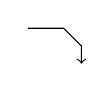
\begin{tikzpicture}[baseline=(O), scale=0.45]
		\coordinate (O) at (0, 0.5);
		\draw[->] (0, 1) -- (1, 1) -- (1.5, 0.5) -- (1.5, 0);
	\end{tikzpicture}$
	合成则给出 $\identity_{X_1^*}$. 明所欲证.
\end{proof}

左对偶和右对偶的相互关系可表作 ${}^* (X^*) = X$ 和 $({}^* X)^* = X$. 尽管在论证或叙述中经常会选定对偶资料, 但对偶性究其实质乃是对象具有的一则性质, 而非外加的结构.

\begin{example}
	在任意幺半范畴中皆有
	\[ \munit^* = \munit = {}^* \munit, \]
	所需的态射 $\mathrm{ev}$ 和 $\mathrm{coev}$ 皆来自幺元约束 $\munit \otimes \munit \simeq \munit$.
\end{example}

\begin{definition}[N.\ Saavedra Rivano]\label{def:rigid-cat}
	\index{yaobanfanchou!刚性 (rigid)}
	若幺半范畴 $\mathcal{C}$ 的所有对象都有左对偶 (或右对偶), 则称 $\mathcal{C}$ 为\emph{左刚性} (或\emph{右刚性}) 范畴.
\end{definition}

\index{xiantu@线图 (string diagram)}
定义--命题 \ref{def:dual-uniqueness} 的证明思路简则简矣, 过程中却引进繁多的公式和交换图表. 在涉及对偶性的各种论证中, 称为\emph{线图}的可视化技巧十分方便; 参照 \S\ref{sec:alg-in-monoidal-cat} 或 \cite[定理 2.6.12 证明]{Li1}. 详言之, 我们以对象为节点, 态射为箭头, 由上而下地合成; 譬如 $\identity_X$, $f: X \to Y$, $g: Y \to Z$ 和 $gf$ 分别表为
\begin{center}\begin{tikzpicture}[morphism/.style={rectangle, draw, fill=white}]
		\node (A) {$X$};
		\node (B) [below=of A] {$X$};
		\path (A) edge (B);
		
		\node (X) [right=of A] {$X$};
		\node (Y) [below=of X] {$Y$};
		\path (X) edge[->] node[midway, morphism] {$f$} (Y);
		
		\node (Y2) [right=of X] {$Y$};
		\node (Z) [right=of Y] {$Z$};
		\path (Y2) edge[->] node[midway, morphism] {$g$} (Z);
		
		\node (X2) [right=of Y2] {$X$};
		\node (Z2) [below=2cm of X2] {$Z$};
		\path (X2) edge[->] node[near start, morphism] {$f$} node[near end, morphism] {$g$} (Z2);
\end{tikzpicture}\end{center}
因此将态射从前或后边合成 $\identity$ 相当于将箭头拉长. 对态射取 $\otimes$ 则表作箭头的并列, 譬如 $f \otimes g$ 表作
\begin{center}\begin{tikzpicture}[morphism/.style={rectangle, draw, fill=white}]
		\node (X) {$X$};
		\node (Y) [right=0.1cm of X] {$Y$};
		\node (Y1) [below=of X] {$Y$};
		\node (Z) [below=of Y] {$Z$};
		\path (X) edge[->] node[midway, morphism] {$f$} (Y1);
		\path (Y) edge[->] node[midway, morphism] {$g$} (Z);
\end{tikzpicture}\end{center}

由于 $X \otimes \munit \simeq X \simeq \munit \otimes X$, 在线图中可以合理地省略 $\munit$, 或者说箭头在该处无端点, 于是在对偶存在的前提下, $\mathrm{ev}: X \otimes X^* \to \munit$ 和 $\mathrm{coev}: \munit \to X^* \otimes X$ 便分别表作
\begin{center}\begin{tikzpicture}[bend angle=70, auto]
		\node (L) {$X$};
		\node (R) [right=of L] {$X^*$};
		\path (L) edge[bend right] node[midway] {$\mathrm{ev}$} (R);
		
		\node (LL) [right=of R] {$X^*$};
		\node (RR) [right=of LL] {$X$};
		\path (LL) edge[bend left] node[midway] {$\mathrm{coev}$} (RR);
\end{tikzpicture}\end{center}

相同前提下, 定义 \ref{def:dualizable-obj} 的等式
\[ (\identity_X \otimes \mathrm{ev}) (\mathrm{coev} \otimes \identity_X ) = \identity_X = (\mathrm{ev} \otimes \identity_X) (\identity_X \otimes \mathrm{coev}) \]
按此图解为
\begin{equation}\label{eqn:Zorro}
	\begin{tikzpicture}[baseline=(B), bend angle=70, auto]
		\node (A) {$X$};
		\node (B) [below=of A] {$X$};
		\node (C) [left=of B] {${}^* X$};
		\node (D) [left=of C] {$X$};
		\node (E) [below=of D] {$X$};
		
		\path (A) edge (B);
		\path (D) edge[bend left] node {$\mathrm{coev}$} (C);
		\path (C) edge[bend right] node {$\mathrm{ev}$} (B);
		
		\path (D) edge[->] (E);
	\end{tikzpicture} \quad = \quad
	\begin{tikzpicture}[baseline=(M)]
		\node (A) {$X$};
		\node (M) [below=of A] {};
		\node (B) [below=of M] {$X$};
		\path (A) edge (B);
		\coordinate (M) at ($(A)!.5!(B)$);
	\end{tikzpicture} \quad = \quad
	\begin{tikzpicture}[baseline=(B), bend angle=70, auto]
		\node (A) {$X$};
		\node (B) [below=of A] {$X$};
		\node (C) [right=of B] {$X^*$};
		\node (D) [right=of C] {$X$};
		\node (E) [below=of D] {$X$};
		
		\path (A) edge (B);
		\path (C) edge[bend left] node {$\mathrm{coev}$} (D);
		\path (B) edge[bend right] node {$\mathrm{ev}$} (C);
		
		\path (D) edge[->] (E);
	\end{tikzpicture}
\end{equation}
前提是所论的对偶存在; 这就赋予定义 \ref{def:dualizable-obj} 一种``拉直箭头''的操作感. 在一些文献中, 上述图表是旋转 $\frac{\pi}{2}$ 后描绘的, 因之又称 \emph{Z 字等式}.
\index{Z-zidengshi@Z 字等式 (mark of Zorro)}

基于代数等式和线图操作之间的这些对应, 涉及对偶性的基本代数等式容易按图索骥, 或者索性以图为证. 作为练习, 读者不妨尝试将定义--命题 \ref{def:dual-uniqueness} 的证明改写成简单的图表.

下一则结果说明对偶自然地调换 $\otimes$ 的次序.

\begin{proposition}
	设 $\mathcal{C}$ 为幺半范畴, $X, Y \in \Obj(\mathcal{C})$.
	\begin{enumerate}[(i)]
		\item 若 $X$ 和 $Y$ 分别有左对偶 ${}^* X$ 和 ${}^* Y$, 则 ${}^* Y \otimes {}^* X$ 给出 $X \otimes Y$ 的左对偶, 相应的资料可以通过 $X$ 和 $Y$ 的对偶资料图解为
		\begin{equation*}
			\mathrm{ev}_{X \otimes Y} = \left[ \begin{tikzcd}[column sep=tiny, ampersand replacement=\&]
				{}^* Y \arrow[dash, rrr, bend right=80, "{\mathrm{ev}_Y}"' near end] \& {}^* X \arrow[dash, r, bend right=60, "{\mathrm{ev}_X}"' near start] \& X \& Y
			\end{tikzcd}\right], \quad
			\mathrm{coev}_{X \otimes Y} = \left[ \begin{tikzcd}[column sep=tiny, ampersand replacement=\&]
				X \arrow[dash, rrr, bend left=80, "{\mathrm{coev}_X}" near start] \& Y \arrow[dash, r, bend left=60, "{\mathrm{coev}_Y}" near end] \& {}^* Y \& {}^* X
			\end{tikzcd}\right].
		\end{equation*}
		\item 若 $X$ 和 $Y$ 分别有右对偶 $X^*$ 和 $Y^*$, 则 $Y^* \otimes X^*$ 给出 $X \otimes Y$ 的右对偶, 相应的资料可以通过 $X$ 和 $Y$ 的对偶资料图解为
		\begin{equation*}
			\mathrm{ev}_{X \otimes Y} = \left[ \begin{tikzcd}[column sep=tiny, ampersand replacement=\&]
				X \arrow[dash, rrr, bend right=80, "{\mathrm{ev}_X}"' near end] \& Y \arrow[dash, r, bend right=60, "{\mathrm{ev}_Y}"' near start] \& Y^* \& X^*
			\end{tikzcd}\right], \quad
			\mathrm{coev}_{X \otimes Y} = \left[ \begin{tikzcd}[column sep=tiny, ampersand replacement=\&]
				X^* \arrow[dash, rrr, bend left=80, "{\mathrm{coev}_X}" near end] \& Y^* \arrow[dash, r, bend left=60, "{\mathrm{coev}_Y}" near start] \& Y \& X
			\end{tikzcd}\right].
		\end{equation*}
	\end{enumerate}
\end{proposition}
\begin{proof}
	必须验证定义 \ref{def:dualizable-obj} 的等式, 亦即 Z 字等式 \eqref{eqn:Zorro}. 这也相当于验证
	\begin{align*}
		\begin{tikzcd}[column sep=tiny, ampersand replacement=\&]
			{}^* Y \arrow[dash, rrr, bend right=80] \& {}^* X \arrow[dash, r, bend right=60] \& X \arrow[dash, rrr, bend left=80] \& Y \arrow[dash, r, bend left=60] \& {}^* Y \& {}^* X
		\end{tikzcd} & = \begin{tikzcd}[column sep=tiny, ampersand replacement=\&]
			{}^* Y \arrow[dash, d] \& {}^* X \arrow[dash, d] \\
			{}^* Y \& {}^* X 
		\end{tikzcd}, \\
		\begin{tikzcd}[column sep=tiny, ampersand replacement=\&]
			X \arrow[dash, rrr, bend left=80] \& Y \arrow[dash, r, bend left=60] \& {}^* Y \arrow[dash, rrr, bend right=80] \& {}^* X \arrow[dash, r, bend right=60] \& X \& Y
		\end{tikzcd} & = \begin{tikzcd}[column sep=tiny, ampersand replacement=\&]
			X \arrow[dash, d] \& Y \arrow[dash, d] \\
			X \& Y 
		\end{tikzcd}
	\end{align*}
	严格来说, 左式的图表应该如 \eqref{eqn:Zorro} 一般往垂直方向拉开, 亦即插入若干 $\identity$, 适当地横挪然后拉直. 上述等式遂一目了然. 相应的形式化验证则是基于幺元的种种自然性质, 细节留给感兴趣的读者.
\end{proof}

\begin{definition}\label{def:dual-morphism}
	\index[sym1]{f-star@$f^*, {}^* f$}
	设 $f: X \to Y$ 是幺半范畴 $\mathcal{C}$ 中的态射. 设 $X$ 和 $Y$ 皆有左对偶 ${}^* X$ 和 ${}^* Y$ (或右对偶 $X^*$ 和 $Y^*$), 此时定义 $f$ 的左对偶 ${}^* f: {}^* Y \to {}^* X$ (或右对偶 $f^*: Y^* \to X^*$) 态射如下:
	\begin{equation*}\begin{aligned}
		{}^* f := (\mathrm{ev}_Y \otimes \identity) (\identity \otimes f \otimes \identity) (\identity \otimes \mathrm{coev}_X) \; &
		\begin{tikzpicture}[baseline=(T), bend angle=70, auto]
			\node (A) {${}^* Y$};
			\node (B) [below=of A] {${}^* Y$};
			\node (C) [right=of B] {$Y$};
			\node (S) [right=of A] {$X$};
			\node[draw, fill=white] (T) at ($(S)!.5!(C)$) {$f$};
			\node (D) [right=of S] {${}^* X$}; 
			\node (E) [below=of D] {${}^* X$};
				
			\path (A) edge (B);
			\path (B) edge[bend right] node {$\mathrm{ev}_Y$} (C);
			\path (C) edge (T);
			\path (T) edge (S);
			\path (S) edge[bend left] node {$\mathrm{coev}_X$} (D);
			\path (D) edge[->] (E);
		\end{tikzpicture}, \\
		f^* := (\identity \otimes \mathrm{ev}_Y) (\identity \otimes f \otimes \identity) (\mathrm{coev}_X \otimes \identity) \; &
		\begin{tikzpicture}[baseline=(T), bend angle=70, auto]
			\node (A) {$Y^*$};
			\node (B) [below=of A] {$Y^*$};
			\node (C) [left=of B] {$Y$};
			\node (S) [left=of A] {$X$};
			\node[draw, fill=white] (T) at ($(S)!.5!(C)$) {$f$};
			\node (D) [left=of S] {$X^*$}; 
			\node (E) [below=of D] {$X^*$};
				
			\path (A) edge (B);
			\path (C) edge[bend right] node {$\mathrm{ev}_Y$} (B);
			\path (C) edge (T);
			\path (T) edge (S);
			\path (D) edge[bend left] node {$\mathrm{coev}_X$} (S);
			\path (D) edge[->] (E);
		\end{tikzpicture}.
	\end{aligned}\end{equation*}
\end{definition}

基于左对偶和右对偶的相互关系和定义--命题 \ref{def:dualizable-obj}, 可以验证 ${}^* (f^*) = f = ({}^* f)^*$; 绘制``图中图''可一目了然. 此外 ${}^* (\identity_X) = \identity_{{}^* X}$ 和 $(\identity_X)^* = \identity_{X^*}$ 则归结为定义.

谨记录两组关于 $f: X \to Y$ 的左/右对偶的有用等式, 依旧以图为证.
\begin{gather}
	\label{eqn:f-dual-coev}
	\begin{tikzpicture}[baseline=(M)]
		\coordinate (A) at (0, 0);
		\coordinate (B) at (1, 0);
		\coordinate (C) at (0, -1);
		\coordinate (D) at (1, -1);
		\draw (C) -- (A) arc[start angle=180, end angle=0, radius=0.5] -- (D);
		\node[draw, fill=white] (M) at ($(A)!.5!(C)$) {$f$};
		\node [below=0.05cm of C] {$Y$};
		\node [below=0.05cm of D] {${}^* X$};
	\end{tikzpicture} = \begin{tikzpicture}[baseline=(M)]
		\coordinate (A) at (0, 0);
		\coordinate (B) at (1, 0);
		\coordinate (C) at (0, -1);
		\coordinate (D) at (1, -1);
		\draw (C) -- (A) arc[start angle=180, end angle=0, radius=0.5] -- (D);
		\node[draw, fill=white] (M) at ($(B)!.5!(D)$) {${}^* f$};
		\node [below=0.05cm of C] {$Y$};
		\node [below=0.05cm of D] {${}^* X$};
	\end{tikzpicture} \qquad \begin{tikzpicture}[baseline=(M)]
		\coordinate (A) at (0, 0);
		\coordinate (B) at (1, 0);
		\coordinate (C) at (0, -1);
		\coordinate (D) at (1, -1);
		\draw (C) -- (A) arc[start angle=180, end angle=0, radius=0.5] -- (D);
		\node[draw, fill=white] (M) at ($(A)!.5!(C)$) {$f^*$};
		\node [below=0.05cm of C] {$X^*$};
		\node [below=0.05cm of D] {$Y$};
	\end{tikzpicture} = \begin{tikzpicture}[baseline=(M)]
		\coordinate (A) at (0, 0);
		\coordinate (B) at (1, 0);
		\coordinate (C) at (0, -1);
		\coordinate (D) at (1, -1);
		\draw (C) -- (A) arc[start angle=180, end angle=0, radius=0.5] -- (D);
		\node[draw, fill=white] (M) at ($(B)!.5!(D)$) {$f$};
		\node [below=0.05cm of C] {$X^*$};
		\node [below=0.05cm of D] {$Y$};
	\end{tikzpicture} \\
	\label{eqn:f-dual-ev}
	\begin{tikzpicture}[baseline=(M)]
		\coordinate (A) at (0, 0);
		\coordinate (B) at (1, 0);
		\coordinate (C) at (0, -1);
		\coordinate (D) at (1, -1);
		\draw (B) -- (D) arc[start angle=360, end angle=180, radius=0.5] -- (A);
		\node[draw, fill=white] (M) at ($(A)!.5!(C)$) {$f$};
		\node [above=0.05cm of A] {$X$};
		\node [above=0.05cm of B] {$Y^*$};
	\end{tikzpicture} \; = \; \begin{tikzpicture}[baseline=(M)]
		\coordinate (A) at (0, 0);
		\coordinate (B) at (1, 0);
		\coordinate (C) at (0, -1);
		\coordinate (D) at (1, -1);
		\draw (B) -- (D) arc[start angle=360, end angle=180, radius=0.5] -- (A);
		\node[draw, fill=white] (M) at ($(B)!.5!(D)$) {$f^*$};
		\node [above=0.05cm of A] {$X$};
		\node [above=0.05cm of B] {$Y^*$};
	\end{tikzpicture} \qquad \begin{tikzpicture}[baseline=(M)]
		\coordinate (A) at (0, 0);
		\coordinate (B) at (1, 0);
		\coordinate (C) at (0, -1);
		\coordinate (D) at (1, -1);
		\draw (B) -- (D) arc[start angle=360, end angle=180, radius=0.5] -- (A);
		\node[draw, fill=white] (M) at ($(A)!.5!(C)$) {${}^* f$};
		\node [above=0.05cm of A] {${}^* Y$};
		\node [above=0.05cm of B] {$X$};
	\end{tikzpicture} \; = \; \begin{tikzpicture}[baseline=(M)]
		\coordinate (A) at (0, 0);
		\coordinate (B) at (1, 0);
		\coordinate (C) at (0, -1);
		\coordinate (D) at (1, -1);
		\draw (B) -- (D) arc[start angle=360, end angle=180, radius=0.5] -- (A);
		\node[draw, fill=white] (M) at ($(B)!.5!(D)$) {$f$};
		\node [above=0.05cm of A] {${}^* Y$};
		\node [above=0.05cm of B] {$X$};
	\end{tikzpicture}
\end{gather}

\begin{proposition}
	设 $X \xrightarrow{f} Y \xrightarrow{g} Z$ 是幺半范畴 $\mathcal{C}$ 中的态射. 设这些对象皆有左对偶 (或右对偶), 则 ${}^* (gf) = {}^* f \; {}^* g$ (或 $(gf)^* = f^* g^*$).
\end{proposition}
\begin{proof}
	运用 Z 字等式 \eqref{eqn:Zorro}, 一图胜千言.
\end{proof}

\begin{corollary}
	对于左刚性 (或右刚性) 范畴 $\mathcal{C}$, 倒转箭头的同时倒转 $\otimes$ 的变元顺序以赋予 $\mathcal{C}^{\opp}$ 幺半结构, 则我们有幺半函子 $\mathcal{C} \to \mathcal{C}^{\opp}$, 映对象 $X$ 为 ${}^* X$ (或 $X^*$), 映态射 $f$ 为 ${}^* f$ (或 $f^*$).
\end{corollary}

出人意料地, 对于从左或右刚性范畴出发的幺半函子, 其间的态射必为同构. 这颇能够说明``刚性''的底蕴.

\begin{proposition}\label{prop:monoidal-functor-rigidity}
	设 $F, G: \mathcal{C} \rightrightarrows \mathcal{D}$ 为幺半范畴之间的幺半函子. 若 $\mathcal{C}$ 是左刚性 (或右刚性) 的, 则幺半函子之间的所有态射 $\varphi: F \to G$ 皆是同构. 事实上, $(\varphi_X)^{-1} = \left(\varphi_{{}^* X}\right)^*$ (或 ${}^* \left( \varphi_{X^*} \right)$).
\end{proposition}
\begin{proof}
	考虑左刚性情形即可. 选定 $X \in \Obj(\mathcal{C})$, 其左对偶 ${}^* X$ 和资料 $\mathrm{ev}$, $\mathrm{coev}$. 我们有交换图表
	\begin{equation*}\begin{gathered}
		\begin{tikzcd}
			\munit \arrow[r, "\sim"] \arrow[rd, "\sim"' sloped] & F(\munit) \arrow[d, "{\varphi_{\munit}}"] \arrow[r, "{F\mathrm{coev}}"] & F(X \otimes {}^* X) \arrow[r, "\sim"] \arrow[d, "{\varphi_{X \otimes {}^* X}}"] & F(X) \otimes F({}^* X) \arrow[d, "{\varphi_X \otimes \varphi_{{}^* X}}"] \\
			& G(\munit) \arrow[r, "{G\mathrm{coev}}"'] & G(X \otimes {}^* X) \arrow[r, "\sim"'] & G(X) \otimes G({}^* X)
		\end{tikzcd} \\
		\begin{tikzcd}
			F({}^* X) \otimes F(X) \arrow[r, "\sim"] \arrow[d, "{\varphi_{{}^* X} \otimes \varphi_X}"'] & F({}^* X \otimes X) \arrow[r, "{F\mathrm{ev}}"] \arrow[d, "{\varphi_{{}^* X \otimes X}}"] & F(\munit) \arrow[r, "\sim"] \arrow[d, "{\varphi_{\munit}}"] & \munit \\
			G({}^* X) \otimes G(X) \arrow[r, "\sim"'] & G({}^* X \otimes X) \arrow[r, "{G\mathrm{ev}}"'] & G(\munit) \arrow[ru, "\sim"' sloped] &
		\end{tikzcd}
	\end{gathered}\end{equation*}
	而且命题 \ref{prop:monoidal-functor-dual} 说明图表按两行的合成分别使 $F({}^* X)$ 和 $G({}^* X)$ 给出 $F(X)$ 和 $G(X)$ 的左对偶; 因此 $(\varphi_{{}^* X})^*: G(X) \to F(X)$ 有定义. 由此得到图表等式

	\begin{equation*}\begin{aligned}
		\begin{tikzpicture}[baseline=(T), bend angle=70, auto]
			\node (A) {$G(X)$};
			\node (B) [below=of A] {$G(X)$};
			\node (C) [left=of B] {$G({}^* X)$};
			\node (S) [left=of A] {$F({}^* X)$};
			\node[draw, fill=white] (T) at ($(S)!.5!(C)$) {$\varphi_{{}^* X}$};
			\node (D) [left=of S] {$F(X)$}; 
			\node (E) [below=of D] {$G(X)$};
				
			\path (A) edge[->] (B);
			\path (C) edge[bend right] node {$G\mathrm{ev}$} (B);
			\path (C) edge (T);
			\path (T) edge (S);
			\path (D) edge[bend left] node {$F\mathrm{coev}$} (S);
			\path (D) edge[->] (E);
			\node[draw, fill=white] at ($(D)!.5!(E)$) {$\varphi_X$};
		\end{tikzpicture} & = \begin{tikzpicture}[baseline=(A)]
			\node (A) {$G(X)$};
			\node (B) [right=of A] {$G({}^* X)$};
			\node (C) [right=of B] {$G(X)$};
			\path (A) edge[bend left=70] node[midway, auto] {$G(\mathrm{coev})$} (B);
			\path (B) edge[bend right=70] node[midway, auto] {$G(\mathrm{ev})$} (C);	
		\end{tikzpicture}, \\
		\begin{tikzpicture}[baseline=(T), bend angle=70, auto]
			\node (A) {$F(X)$};
			\node (B) [below=of A] {$G(X)$};
			\node (C) [left=of B] {$G({}^* X)$};
			\node (S) [left=of A] {$F({}^* X)$};
			\node[draw, fill=white] (T) at ($(S)!.5!(C)$) {$\varphi_{{}^* X}$};
			\node (D) [left=of S] {$F(X)$}; 
			\node (E) [below=of D] {$F(X)$};
				
			\path (A) edge[->] (B);
			\path (C) edge[bend right] node {$G\mathrm{ev}$} (B);
			\path (C) edge (T);
			\path (T) edge (S);
			\path (D) edge[bend left] node {$F\mathrm{coev}$} (S);
			\path (D) edge[->] (E);
			\node[draw, fill=white] at ($(A)!.5!(B)$) {$\varphi_X$};
		\end{tikzpicture} & = \begin{tikzpicture}[baseline=(A)]
			\node (A) {$F(X)$};
			\node (B) [right=of A] {$F({}^* X)$};
			\node (C) [right=of B] {$F(X)$};
			\path (A) edge[bend left=70] node[midway, auto] {$F(\mathrm{coev})$} (B);
			\path (B) edge[bend right=70] node[midway, auto] {$F(\mathrm{ev})$} (C);	
		\end{tikzpicture},
	\end{aligned}\end{equation*}
	右侧根据 \eqref{eqn:Zorro} 分别是 $\identity_{GX}$ 和 $\identity_{FX}$. 这便说明 $\left(\varphi_{{}^* X}\right)^*$ 确实是 $\varphi_X$ 的逆.
\end{proof}

\begin{proposition}\label{prop:dual-internal-Hom}
	设 $\mathcal{C}$ 为幺半范畴而 $X, Y \in \Obj(\mathcal{C})$.
	\begin{enumerate}[(i)]
		\item 当 $X$ 有左对偶 ${}^* X$ 时, 有互逆双射 $\Hom_{\mathcal{C}}(X, Y) \xleftrightarrow{1:1} \Hom_{\mathcal{C}}(\munit, Y \otimes {}^* X)$ 如下.
		\begin{equation*}\begin{aligned}
			\begin{tikzpicture}[baseline=(M)]
				\node (A) {$X$};
				\node (B) [below=of A]{$Y$};
				\path (A) edge[->] node[midway, draw, fill=white] {$f$} (B);
				\coordinate (M) at ($(A)!.5!(B)$);
			\end{tikzpicture}
			& \; \longmapsto \; \begin{tikzpicture}[baseline=(B), bend angle=70]
				\node (A) {$X$};
				\node (B) [right=of A] {${}^* X$};
				\node (C) [below=of A] {$Y$};
				\node (D) [below=of B] {${}^* X$};
				\path (A) edge[bend left] node[auto] {$\mathrm{coev}_X$} (B);
				\path (A) edge[->] node[midway, draw, fill=white] {$f$} (C);
				\path (B) edge (D);
			\end{tikzpicture}
			\\
			\begin{tikzpicture}[baseline=(D), bend angle=70]
				\node (B) {$X$};
				\node (C) [left=of B] {${}^* X$};
				\node (D) [left=of C] {$Y$};
				\node (A) [below=of D] {$Y$};
				\path (D) edge[->] (A);
				\path (C) edge[bend right] node[auto] {$\mathrm{ev}_X$} (B);
				\path (D) edge[bend left] node[midway, draw, fill=white] {$\varphi$} (C);
			\end{tikzpicture}
			& \; \longmapsfrom \;
			\begin{tikzpicture}[baseline=(A), bend angle=70]
				\node (A) {$Y$};
				\node (B) [right=of A] {${}^* X$};
				\path (A) edge[bend left] node[midway, draw, fill=white] {$\varphi$} (B);
			\end{tikzpicture}
		\end{aligned}\end{equation*}
		\item 当 $X$ 有右对偶 $X^*$ 时, 有互逆双射 $\Hom_{\mathcal{C}}(X, Y) \xleftrightarrow{1:1} \Hom_{\mathcal{C}}(\munit, X^* \otimes Y)$ 如下.
		\begin{equation*}\begin{aligned}
			\begin{tikzpicture}[baseline=(M)]
				\node (A) {$X$};
				\node (B) [below=of A]{$Y$};
				\path (A) edge[->] node[midway, draw, fill=white] {$f$} (B);
				\coordinate (M) at ($(A)!.5!(B)$);
			\end{tikzpicture}
			& \; \longmapsto \; \begin{tikzpicture}[baseline=(B), bend angle=70]
				\node (A) {$X$};
				\node (B) [left=of A] {$X^*$};
				\node (C) [below=of A] {$Y$};
				\node (D) [below=of B] {$X^*$};
				\path (B) edge[bend left] node[auto] {$\mathrm{coev}_X$} (A);
				\path (A) edge[->] node[midway, draw, fill=white] {$f$} (C);
				\path (B) edge (D);
			\end{tikzpicture}
			\\
			\begin{tikzpicture}[baseline=(D), bend angle=70]
				\node (B) {$X$};
				\node (C) [right=of B] {$X^*$};
				\node (D) [right=of C] {$Y$};
				\node (A) [below=of D] {$Y$};
				\path (D) edge[->] (A);
				\path (B) edge[bend right] node[auto] {$\mathrm{ev}_X$} (C);
				\path (C) edge[bend left] node[midway, draw, fill=white] {$\varphi$} (D);
			\end{tikzpicture}
			& \; \longmapsfrom \;
			\begin{tikzpicture}[baseline=(A), bend angle=70]
				\node (A) {$X^*$};
				\node (B) [right=of A] {$Y$};
				\path (A) edge[bend left] node[midway, draw, fill=white] {$\varphi$} (B);
			\end{tikzpicture}
		\end{aligned}\end{equation*}
		\item 推而广之, 在所论对偶存在的前提下, 存在典范双射
		\[\begin{tikzcd}[row sep=tiny]
			\Hom_{\mathcal{C}}\left( W \otimes X, Y \right) \arrow[r, "1:1"] & \Hom_{\mathcal{C}}(W, Y \otimes {}^* X) \\
			f \arrow[mapsto, r] & (f \otimes \identity_{{}^* X}) (\identity_W \otimes \mathrm{coev}_X)
		\end{tikzcd}\]
		和
		\[\begin{tikzcd}
			\Hom_{\mathcal{C}}\left( X \otimes W, Y \right) \arrow[r, "1:1"] & \Hom_{\mathcal{C}}(W, X^* \otimes Y) \\
			f \arrow[mapsto, r] & (\identity_{X^*} \otimes f) (\mathrm{coev}_X \otimes \identity_W).
		\end{tikzcd}\]
	\end{enumerate}
\end{proposition}
\begin{proof}
	对于 (i) 和 (ii), 互逆的验证不外是 \eqref{eqn:Zorro} 的应用. 基于同样思路, 但画法稍加别扭的图表足以解释 (iii).
\end{proof}

在 (i) 和 (ii) 的情境下, 容易将态射的合成在双射右侧的元素 $\varphi$ 上描述 (提示: 应用态射 $\mathrm{ev}$). 这些典范操作引向以下结果.

\begin{corollary}\label{prop:rigid-Hom-internal}
	\index[sym1]{Hom-internal}
	设 $\mathcal{C}$ 是定义 \ref{def:rigid-cat} 所谓的左刚性 (或右刚性) 范畴, 则定义内 $\Hom$ 为 $\iHom_{\text{左}}(X, Y) := Y \otimes {}^* X$ (或 $\iHom_{\text{右}}(X, Y) := X^* \otimes Y$) 可使 $\mathcal{C}$ 成为定义 \ref{def:closed-monoidal-cat} 所谓的右 (或左) 闭幺半范畴.
\end{corollary}
\begin{proof}
	将命题 \ref{prop:dual-internal-Hom} (iii) 代入定义 \ref{def:closed-monoidal-cat}, 其余验证全是例行公事.
\end{proof}

\begin{corollary}\label{prop:rigid-exact}
	设 $X \in \Obj(\mathcal{C})$.
	\begin{itemize}
		\item 若 $X$ 有左对偶 ${}^* X$, 则 $(\cdot) \otimes X$ 保小 $\varinjlim$ 而 $X \otimes (\cdot)$ 保小 $\varprojlim$.
		\item 若 $X$ 有右对偶 $X^*$, 则 $(\cdot) \otimes X$ 保小 $\varprojlim$ 而 $X \otimes (\cdot)$ 保小 $\varinjlim$.
	\end{itemize}
\end{corollary}
\begin{proof}
	考虑 $X$ 有左对偶 ${}^* X$ 的情形. 命题 \ref{prop:dual-internal-Hom} (iii) 蕴涵函子 $(\cdot) \otimes X$ 有右伴随 $(\cdot) \otimes {}^* X$, 函子 $X \otimes (\cdot) \simeq ({}^* X)^* \otimes (\cdot)$ 有左伴随 ${}^* X \otimes (\cdot)$.
	
	在上述论证中调换 $\otimes$ 的顺序, 即可处理有右对偶 $X^*$ 的情形.
\end{proof}

\section{对偶性: 迹和维数}\label{sec:symm-monoidal-dual}
我们在 \S\ref{sec:monoidal-dual} 介绍了和对偶性相关的几则概念, 它们都分成左/右两种版本, 取决于对象在 $\otimes$ 中的位置. 许多应用中考虑的幺半范畴是对称的, 这时不必再区分左右. 我们且从辫幺半范畴的情况入手. 辫结构照例写作
\[ c(X,Y): X \otimes Y \rightiso Y \otimes X \]
的形式, 辫结构对称相当于说 $c(X, Y)^{-1} = c(Y, X)$. 辫图可以和 \S\ref{sec:monoidal-dual} 介绍的线图技巧搭配使用.

\begin{lemma}\label{prop:braided-dual}
	设 $\mathcal{C}$ 是辫幺半范畴. 给定 $X \in \Obj(\mathcal{C})$ 的右对偶 $X^*$, 则 $X^*$ 也是 $X$ 的左对偶; 精确地说, 命
	\begin{align*}
		\mathrm{ev}' & := \mathrm{ev} \circ c(X, X^*)^{-1}: X^* \otimes X \to \munit, \\
		\mathrm{coev}' & := c(X^*, X) \circ \mathrm{coev}: \munit \to X \otimes X^* ,
	\end{align*}
	则 $(X^*, X, \mathrm{ev}', \mathrm{coev}')$ 是对偶资料. 左对偶 ${}^* X$ 的情形类此. 当 $\mathcal{C}$ 是对称幺半范畴时, 我们进一步有 $\mathrm{ev}'' = \mathrm{ev}$ 和 $\mathrm{coev}'' = \mathrm{coev}$.
\end{lemma}
\begin{proof}
	这是辫结构的公理的应用. 举例明之, $(\identity \otimes \mathrm{ev}') (\mathrm{coev}' \otimes \identity) = \identity$ 归结为下图交换:
	\[\begin{tikzcd}
		X \otimes \munit \arrow[d, "{c(X, \munit)}"] \arrow[r, "{\identity \otimes \mathrm{coev}}"] & X \otimes X^* \otimes X \arrow[d, "{c(X, X^* \otimes X)}"] \arrow[rrr, "{\mathrm{ev} \otimes \identity}"] & & & \munit \otimes X \arrow[d, "{c(\munit, X)}"'] \\
		\munit \otimes X \arrow[r, "{\mathrm{coev} \otimes \identity}"' inner sep=0.6em] & X^* \otimes X \otimes X \arrow[r, "{c(X^*, X) \otimes \identity}"' inner sep=0.6em] & X \otimes X^* \otimes X \arrow[r, "{\identity \otimes c(X, X^*)^{-1}}"' inner sep=0.6em] & X \otimes X \otimes X^* \arrow[r, "{\identity \otimes \mathrm{ev}}"' inner sep=0.6em] & X \otimes \munit
	\end{tikzcd}\]
	小方块交换缘于辫结构的函子性, 右侧大方块则是例行的辫图论证, 可参照 \S\ref{sec:alg-in-monoidal-cat}.
\end{proof}

综上, 辫幺半范畴的对象 $X$ 有左对偶当且仅当它有右对偶. 对于对称幺半范畴的情形, 我们可以放心地混同左右, 将对偶对象和对偶态射统一记为 $X^*$ 和 $f^*$.

最为典型的例子当然是交换环上的模范畴, 它对模的张量积构成对称幺半范畴, 其中的对偶性有简单的刻画.

\begin{proposition}\label{prop:dualizable-module}
	设 $R$ 为交换环. 将 $R\dcate{Mod}$ 通过 $\otimes_R$ 作成对称幺半范畴, 则 $R$-模 $M$ 有对偶 $M^*$ 当且仅当 $M$ 是有限生成投射模, 而且此时可取 $M^* := \Hom_R(M, R)$, 而 $\mathrm{ev}_M$ 和 $\mathrm{coev}_M$ 则如定义 \ref{def:bimodule-ev-coev} 所述 (取 $A=B=\Bbbk=R$, $P=M$, 此处的 $M^*$ 在该处记为 $M^\vee$), 至多差一个张量积换序.
\end{proposition}
\begin{proof}
	较为容易的是``当''的方向, 因为 $(M^*, \mathrm{ev}_M, \mathrm{coev}_M)$ 的取法明确. 对于特例 $M = R$, 我们可以等同 $M^*$ 与 $R$, 而 $\mathrm{ev}_M(x \otimes y) = xy$, $\mathrm{coev}_M(1) = 1 \otimes 1$, 此时所需等式的验证都是标准的.
	
	其次, 易见 $(M^*, \mathrm{ev}_M, \mathrm{coev}_M)$ 的给法兼容于直和, 由此可得 $M = R^{\oplus n}$ 的情形. 一般的有限生成投射模 $M$ 总能实现为某个 $R^{\oplus n}$ 的直和项, 由此可得 $M$ 有对偶.
	
	现在考虑``仅当''方向. 设 $R$-模 $M$ 有对偶 $M^*$. 基于命题 \ref{prop:dual-internal-Hom} (ii), 对于任意 $R$-模 $M'$ 皆有 $R$-模同构
	\[\begin{tikzcd}[row sep=tiny]
		\Hom_R(M, M') & \Hom_R(R, M^* \dotimes{R} M') \arrow[l, "\sim"'] \arrow[r, "\sim"] & M^* \dotimes{R} M' \\
		(\mathrm{ev}_M \otimes \identity_{M'}) (\identity_M \otimes \varphi) & \varphi \arrow[mapsto, l] \arrow[mapsto, r] & \varphi(1).
	\end{tikzcd}\]
	
	取 $M' = R$ 可见 $\Hom_R(M, R) \simeq \Hom_R(R, M^*) \simeq M^*$, 它映 $\lambda \in M^*$ 为以下同态:
	\[\begin{tikzcd}[row sep=tiny]
		M \arrow[r, "\sim"] & M \dotimes{R} R \arrow[r, "{\identity_M \otimes \lambda}"] & M \dotimes{R} M^* \arrow[r, "{\mathrm{ev}_M}"] & R \\ 
		m \arrow[mapsto, r] & m \otimes 1 \arrow[mapsto, r] & m \otimes \lambda \arrow[mapsto, r] & \mathrm{ev}_M(m \otimes \lambda).
	\end{tikzcd}\]
	因此 $M^*$ 可等同于 $\Hom_R(M, R)$, 同时 $\mathrm{ev}_M$ 等同于求值.
	
	考察等式 $(\mathrm{ev}_M \otimes \identity_M)(\identity_M \otimes \mathrm{coev}_M) = \identity_M$. 设 $\mathrm{coev}_M(1) = \sum_{i=1}^n \lambda_i \otimes m_i$, 等式相当于说 $\sum_i \lambda_i(m) m_i = m$ 恒成立, 亦即 $\identity_M$ 分解为
	\[ M \xrightarrow{(\lambda_1, \ldots, \lambda_n)} R^{\oplus n} \xrightarrow{(m_1, \ldots, m_n)} M, \]
	这说明 $M$ 是 $R^{\oplus n}$ 的直和项. 证毕.
\end{proof}

\begin{definition}\label{def:rigid-cat-braided}
	\index{yaobanfanchou!刚性 (rigid)}
	对于辫幺半范畴, 定义 \ref{def:rigid-cat} 的左刚性和右刚性相互等价; 满足其中任何一者的辫幺半范畴称为\emph{刚性范畴}.
\end{definition}

一旦加上 Abel 范畴结构, 刚性辫幺半范畴的幺元便折射出特殊的性质. 我们首先证明此时 $\otimes$ 对每个变元都自动具有加性.

\begin{proposition}\label{prop:rigid-additive}
	设 $\mathcal{C}$ 是刚性辫幺半范畴. 若 $\mathcal{C}$ 还是加性范畴, 则 $\otimes$ 是加性双函子.
\end{proposition}
\begin{proof}
	选定 $X \in \Obj(\mathcal{C})$. 命题 \ref{prop:dual-internal-Hom} (iii) 蕴涵函子 $X \otimes (\cdot)$ 有右伴随 $X^* \otimes (\cdot)$, 故推论 \ref{prop:automatic-additivity} (v) 确保 $X \otimes (\cdot)$ 具有加性. 基于辫结构, $(\cdot) \otimes X$ 亦然.
\end{proof}

\begin{proposition}\label{prop:rigid-unit-simple}
	设 $\mathcal{C}$ 是刚性辫幺半范畴, 兼具 Abel 范畴的结构. 若 $\iota: U \hookrightarrow \munit$ 是子对象, 则 $\munit = U \oplus \Ker(\iota^*)$. 作为推论:
	\begin{enumerate}[(i)]
		\item 对象 $\munit$ 分裂 (定义 \ref{def:semisimple});
		\item 若 $\End_{\mathcal{C}}(\munit)$ 是域, 则 $\munit$ 是单对象.
	\end{enumerate}
\end{proposition}
\begin{proof}
	命 $V := \Coker(\iota)$. 已知 $\otimes$ 对每个变元都是正合加性函子 (推论 \ref{prop:rigid-exact} 和命题 \ref{prop:rigid-additive}), 故有实线部分的行正合交换图表
	\[\begin{tikzcd}
		0 \arrow[r] & U \arrow[r, "\iota"] & \munit \arrow[r] & V \arrow[r] & 0 \\
		0 \arrow[r] & U \otimes U \arrow[hookrightarrow, u, "{\iota \otimes \identity}"] \arrow[r, "{\identity \otimes \iota}"'] & U \arrow[hookrightarrow, u, "\iota"] \arrow[r] \arrow[dashed, ru] & U \otimes V \arrow[hookrightarrow, u, "{\iota \otimes \identity}"'] \arrow[r] & 0
	\end{tikzcd}\]
	虚线合成箭头为 $0$, 由此知 $U \otimes V = 0$ 而 $U \otimes U \simeq U$.
	
	对任意对象 $T$, 同理可得单态射 $\iota \otimes \identity_T : U \otimes T \hookrightarrow T$, 故 $U \otimes T = 0 \iff \iota \otimes \identity_T = 0$, 而右式又等价于在命题 \ref{prop:dual-internal-Hom} (iii) 之下对应的态射 $T \to U^* \otimes T$ 为 $0$, 不难说明后者正是 $\iota^* \otimes \identity_T$ (本章习题). 综上, 对于任意对象 $X$, 使得 $U \otimes T = 0$ 的极大子对象 $T \subset X$ 等于使得 $T \to U^* \otimes T \hookrightarrow U^* \otimes X$ 为 $0$ 的极大子对象, 这也等于
	\[ \Ker\left[ \iota^* \otimes \identity_X: X \to U^* \otimes X \right] \simeq \Ker(\iota^*) \otimes X. \]
	\begin{itemize}
		\item 施此于 $X = V$ 并利用 $U \otimes V = 0$, 可得 $\Ker(\iota^*) \otimes V \simeq V$;
		\item 施此于 $X = U$, 则因为 $U$ 的子对象 $T$ 也是 $\munit$ 的子对象, 故 $U \otimes T \supset T \otimes T \simeq T$, 由此得 $\Ker(\iota^*) \otimes U = 0$.
	\end{itemize}
	
	将此代入短正合列 
	\[ 0 \to \Ker(\iota^*) \otimes U \to \Ker(\iota^*) \to \Ker(\iota^*) \otimes V \to 0, \]
	立见 $\munit \supset \Ker(\iota^*) \rightiso V$. 这使 $0 \to U \to \munit \to V \to 0$ 分裂. 由于子对象 $U$ 是任意的, 这也正是 $\munit$ 分裂的定义.
	
	最后, 推论 \ref{prop:indecomposable-criterion} 蕴涵当 $\End_{\mathcal{C}}(\munit)$ 是域时 $\munit$ 不可分解, 故 $\munit$ 单.
\end{proof}

任意幺半范畴 $\mathcal{C}$ 中的 $\End(\munit)$ 是幺半群, 容易证明它还是交换的, 见 \cite[第三章习题]{Li1}. 幺约束 $X \simeq \munit \otimes X$ 使得 $\End(\munit)$ 的元素以自态射作用在每个 $X$ 上; 这些自态射确定幺半群同态 $\End(\munit) \to Z(\mathcal{C})$, 此处 $Z(\mathcal{C})$ 代表范畴 $\mathcal{C}$ 的中心. 基于中心的一般性质, 态射合成相对于 $\End(\munit)$ 作用是双线性的:
\[ (z f) g = z(f g) = f (z g), \quad X \xrightarrow{g} Y \xrightarrow{f} Z, \quad z \in \End(\munit). \]

此外, 从 $\otimes$ 的公理 (见 \cite[\S 3.1]{Li1}) 不难导出 $\otimes$ 同样是双线性的:
\[ (zf_1) \otimes f_2 = z(f_1 \otimes f_2) = f_1 \otimes (z f_2), \quad f_i \in \Hom(X_i, Y_i), \quad z \in \End(\munit). \]

不妨设想 $\End(\munit)$ 为幺半范畴 $\mathcal{C}$ 提供了某种``系数''.

\begin{definition}
	\index{ji@迹 (trace)}
	设 $f \in \End(X)$ 是辫幺半范畴 $\mathcal{C}$ 中的自态射, $X$ 有对偶; 定义 $f$ 的左迹 (简称\emph{迹}) 为
	\[ \Tr(f) = \Tr_{\text{左}}(f) := \mathrm{ev}_X \left( f \otimes \identity_{X^*} \right) \mathrm{coev}'_X \; \in \End(\munit), \]
	其右迹定义为
	\[ \Tr_{\text{右}}(f) := \mathrm{ev}'_X \left( \identity_{X^*} \otimes f \right) \mathrm{coev}_X, \]
	其中 $\mathrm{coev}'_X$ 和 $\mathrm{ev}'_X$ 如引理 \ref{prop:braided-dual}; 鉴于定义--命题 \ref{def:dual-uniqueness}, 两种迹不依赖对偶资料的选取.
\end{definition}

\begin{definition}
	\index{weishu@维数 (dimension)}
	设 $X$ 是辫幺半范畴 $\mathcal{C}$ 的对象, $X$ 有对偶, 则其左维数 (简称\emph{维数}) 定义为
	\[ \dim X = \dim_{\text{左}} X := \Tr(\identity_X) \; \in \End(\munit), \]
	其右维数定义为 $\dim_{\text{右}} X := \Tr_{\text{右}}(\identity_X)$.
\end{definition}

左迹和右迹分别图解如下:
\[\Tr_{\text{左}}(f) = \begin{tikzpicture}[baseline=(M), bend angle=70]
	\node (A) {$X$};
	\node (B) [right=of A] {$X^*$};
	\node (C) [below=of A] {$X$};
	\node (D) [below=of B] {$X^*$};
	
	\path (A) edge[bend left] node[auto] {$\mathrm{coev}'_X$} (B);
	\path (B) edge (D);
	\path (A) edge node[midway, name=M, draw, fill=white] {$f$} (C);
	\path (D) edge[bend left] node[auto, swap] {$\mathrm{ev}_X$} (C);
\end{tikzpicture}
\xlongequal{\text{简记}}\;
\begin{tikzpicture}[baseline=(M)]
	\coordinate (A) at (0, 0);
	\coordinate (B) at (1, 0);
	\coordinate (C) at (0, -1);
	\coordinate (D) at (1, -1);
	\draw (A) arc[start angle=180, end angle=0, radius=0.5] -- (D) arc[start angle=360, end angle=180, radius=0.5] -- (A);
	\node[draw, fill=white] (M) at ($(A)!.5!(C)$) {$f$};
\end{tikzpicture} \qquad
\Tr_{\text{右}}(f) \xlongequal{\text{简记}}\; \begin{tikzpicture}[baseline=(M)]
	\coordinate (A) at (0, 0);
	\coordinate (B) at (1, 0);
	\coordinate (C) at (0, -1);
	\coordinate (D) at (1, -1);
	\draw (A) arc[start angle=175, end angle=0, radius=0.5] -- (D) arc[start angle=360, end angle=180, radius=0.5] -- (A);
	\node[draw, fill=white] (M) at ($(B)!.5!(D)$) {$f$};
\end{tikzpicture}\]

若 $\mathcal{C}$ 是对称幺半范畴, 则左右两种版本的迹和维数总是相等, 这也是未来的主要应用场景.

必须突出范畴 $\mathcal{C}$ 的角色时, 我们将采用 $\Tr_{\mathcal{C}}$ 和 $\dim_{\mathcal{C}}$ 等记法. 一些文献也称之为量子迹和量子维数. 例 \ref{eg:Vect-trace} 将说明它们和经典版本的关系.

\begin{proposition}
	设 $F: \mathcal{C} \to \mathcal{D}$ 为辫幺半范畴之间的幺半函子, 保持辫结构, 则对 $\mathcal{C}$ 的任何自态射 $f \in \End(X)$, 在 $X$ 有对偶的前提下 $F\left(\Tr_{\mathcal{C}}(f)\right) = \Tr_{\mathcal{D}}(Ff)$; 考虑右迹亦然. 特别地, $F\left( \dim_{\mathcal{C}} X \right) = \dim_{\mathcal{D}}(FX)$.
\end{proposition}
\begin{proof}
	和命题 \ref{prop:monoidal-functor-dual} 全同. 
\end{proof}

以上定义的迹具有和线性映射的迹相类似的性质.

\begin{proposition}\label{prop:trace}
	设 $\mathcal{C}$ 为辫幺半范畴. 以下讨论自态射 $f \in \End(X)$ 时皆默认 $X$ 有对偶.
	\begin{enumerate}[(i)]
		\item 我们有 $\Tr_{\text{左}}(f) = \Tr_{\text{右}}({}^* f)$ 和 $\Tr_{\text{右}}(f) = \Tr_{\text{左}}(f^*)$.
		\item 设 $X$ 和 $Y$ 皆有对偶. 对任意
		$\begin{tikzcd} X \arrow[shift left, r, "f"] & Y \arrow[shift left, l, "g"] \end{tikzcd}$,
		我们有 $\Tr_{\text{左}}\left( gf \right) = \Tr_{\text{左}}\left(({}^{**} f) g\right)$ 和 $\Tr_{\text{右}}\left( gf \right) = \Tr_{\text{右}}\left((f^{**}) g\right)$. 留意到当 $\mathcal{C}$ 是对称幺半范畴时, ${}^{**} f = f = f^{**}$.
		\item 对任意 $f \in \End(X)$ 和 $g \in \End(Y)$, 我们有 $\Tr(f \otimes g) = \Tr(f)\Tr(g)$.
		\item 设 $a \in \End(\munit)$, 则 $\Tr(af) = a\Tr(f)$ 恒成立.
		\item 设 $\mathcal{C}$ 是 $\cate{Ab}$-范畴, 而且 $\otimes$ 对第一个 (或第二个) 变元具有加性, 则对任意 $f, g \in \End(X)$ 皆有 $\Tr_{\text{左}}(f + g) = \Tr_{\text{左}}(f) + \Tr_{\text{左}}(g)$ (或 $\Tr_{\text{右}}(f + g) = \Tr_{\text{右}}(f) + \Tr_{\text{右}}(g)$).
	\end{enumerate}
	断言 (iii) 和 (iv) 中的 $\Tr$ 既可以代入左迹, 也可以代入右迹.
\end{proposition}
\begin{proof}
	按照往例, 我们主要依赖图形来论证. 基于对称性, 讨论左迹即可. 首先, 基于迹的图解, 对 \eqref{eqn:f-dual-coev} 的各项装配底盘即得 (i). 类似道理, (ii) 通过 \eqref{eqn:f-dual-ev} 图解如下.
	\[\begin{tikzpicture}[baseline=(O)]
		\coordinate (A) at (0, 0);
		\coordinate (B) at (1, 0);
		\coordinate (C) at (0, -1);
		\coordinate (D) at (1, -1);
		\coordinate (O) at (0, -0.5);
		\draw (A) arc[start angle=180, end angle=0, radius=0.5] -- (D) arc[start angle=360, end angle=180, radius=0.5] -- (A);
		\node[draw, fill=white] (M) at ($(A)!.2!(C)$) {$f$};
		\node[draw, fill=white] (N) at ($(A)!.8!(C)$) {$g$};
	\end{tikzpicture} = \begin{tikzpicture}[baseline=(O)]
		\coordinate (A) at (0, 0);
		\coordinate (B) at (1, 0);
		\coordinate (C) at (0, -1);
		\coordinate (D) at (1, -1);
		\coordinate (O) at (0, -0.5);
		\draw (A) arc[start angle=180, end angle=0, radius=0.5] -- (D) arc[start angle=360, end angle=180, radius=0.5] -- (A);
		\node[draw, fill=white] (M) at ($(B)!.5!(D)$) {${}^* f$};
		\node[draw, fill=white] (N) at ($(A)!.5!(C)$) {$g$};
	\end{tikzpicture} = \begin{tikzpicture}[baseline=(O)]
		\coordinate (A) at (0, 0);
		\coordinate (B) at (1, 0);
		\coordinate (C) at (0, -1);
		\coordinate (D) at (1, -1);
		\coordinate (O) at (0, -0.5);
		\draw (A) arc[start angle=180, end angle=0, radius=0.5] -- (D) arc[start angle=360, end angle=180, radius=0.5] -- (A);
		\node[draw, fill=white] (M) at ($(A)!.2!(C)$) {$g$};
		\node[draw, fill=white] (N) at ($(A)!.8!(C)$) {${}^{**} f$};
	\end{tikzpicture}\]
	
	对于 (iii), 关键是直观的等式
	\[\begin{tikzpicture}[baseline=(O)]
		\coordinate (O) at (0, 0);
		\draw (O) circle[radius=1];
		\draw (O) circle[radius=0.4];
		\node[draw, fill=white] at ($(O) + (180:1)$) {$f$};
		\node[draw, fill=white] at ($(O) + (180:0.4)$) {$g$};
	\end{tikzpicture} \; = \;
	\begin{tikzpicture}[baseline=(A)]
		\coordinate (A) at (0, 0);
		\coordinate (B) at (1.2, 0);
		\draw (A) circle[radius=0.4];
		\draw (B) circle[radius=0.4];
		\node[draw, fill=white] at ($(A) + (180:0.4)$) {$f$};
		\node[draw, fill=white] at ($(B) + (180:0.4)$) {$g$};
	\end{tikzpicture} \; = \;
	\begin{tikzpicture}[baseline=(O)]
		\coordinate (A) at (0, 1);
		\coordinate (B) at (0, 0);
		\coordinate (O) at ($(A)!.5!(B)$);
		\draw (A) circle[radius=0.4];
		\draw (B) circle[radius=0.4];
		\node[draw, fill=white] at ($(A) + (180:0.4)$) {$f$};
		\node[draw, fill=white] at ($(B) + (180:0.4)$) {$g$};
	\end{tikzpicture}\]
	其形式证明则是基于幺元的种种自然性质.
	
	断言 (iv) 来自态射合成与 $\otimes$ 相对于 $\End(\munit)$ 的双线性性质. 断言 (v) 则直接来自左迹和右迹的文字定义, 不必图解.
\end{proof}

不妨将命题 \ref{prop:trace} (iv) 和 (v) 理解为迹的线性性质. 作为 (iii) 的特例, 我们也有 $\dim X \otimes Y = \dim X \dim Y$.

\section{对偶性的实例}\label{sec:duality-examples}
我们接着来考察对偶性理论的若干基本实例.

\begin{example}\label{eg:Vect-trace}
	考虑域 $\Bbbk$ 上的向量空间范畴 $\cate{Vect}(\Bbbk)$ 及其标准的对称幺半结构, 其幺元为 $\munit := \Bbbk$. 这是对偶性的模板. 命题 \ref{prop:dualizable-module} 蕴涵对于任意 $\Bbbk$-向量空间 $V$,
	\[ V \;\text{有对偶} \iff V \;\text{有限维}. \]
	更具体地说, 对于 $n$ 维 $\Bbbk$-向量空间 $V$, 其对偶 (不必分左右) 取为
	\[ V^* := \Hom_{\Bbbk}(V, \Bbbk), \]
	对应的态射是
	\[\begin{tikzcd}[row sep=tiny]
		V \otimes V^* \arrow[r, "{\mathrm{ev}}"] & \Bbbk \\
		v \otimes \check{v} \arrow[mapsto, r] & \check{v}(v)
	\end{tikzcd} \quad \begin{tikzcd}[row sep=tiny]
		\Bbbk \arrow[r, "{\mathrm{coev}}"] & V^* \otimes V \\
		1 \arrow[mapsto, r] & \sum_{i=1}^n \check{v}_i \otimes v_i
	\end{tikzcd} \]
	其中 $v_1, \ldots, v_n$ 是 $V$ 的任意基, $\check{v}_1, \ldots, \check{v}_n$ 则是其对偶基. 这些定义既是命题 \ref{prop:dualizable-module} 的特例, 直接验证也毫无困难.
	
	\index[sym1]{Vectf@$\cate{Vect}_{\mathrm{f}}$}
	有限维 $\Bbbk$-向量空间对 $\otimes$ 成为刚性范畴, 记为 $\cate{Vect}_{\mathrm{f}}(\Bbbk)$. 涉及对偶的所有操作都化作常识, 勾勒如下.
	\begin{itemize}
		\item 同构 $V^* \otimes W \simeq \Hom(\Bbbk, V^* \otimes W) \rightiso \Hom(V, W)$ 映 $\sum_i \check{v}_i \otimes w_i$ 为线性映射 $\sum_i \check{v}_i(\cdot) w_i$.
		\item 态射 $f: V \to W$ 的对偶 $f^*: W^* \to V^*$ 无非是线性映射的转置, 图表等式 \eqref{eqn:f-dual-ev}	道尽一切.
		\item 迹和维数取值在 $\End(\Bbbk) \simeq \Bbbk$. 既然 $\cate{Vect}_{\mathrm{f}}(\Bbbk)$ 对称, 免分左右.
		\item 等同 $\End(V)$ 和 $V^* \otimes V$, 则 $\Tr(\sum_i \check{v}_i \otimes v_i) = \sum_i \check{v}_i(v_i)$ 正是经典的迹. 同理, $\dim V$ 无非是经典维数在同态 $\Z \to \Bbbk$ 之下的像.
	\end{itemize}
\end{example}

\begin{example}\label{eg:superVect-trace}
	\index{chaoxiangliangkongjian}
	考虑例 \ref{eg:superspace} 的对称幺半范畴 $\cate{Vect}^-_{\Z/2\Z}(\Bbbk)$, 其对象 (或态射) 写作 $V = V_0 \oplus V_1$ (或 $f = (f_0, f_1)$) 之形, 以 $\Bbbk = \Bbbk \oplus \{0\}$ 为幺元. 一如例 \ref{eg:Vect-trace}, 对象 $V$ 有对偶当且仅当 $V$ 是有限维 $\Bbbk$-向量空间; 这些空间构成全子范畴 $\cate{Vect}^-_{\Z/2\Z, f}(\Bbbk)$. 当 $V$ 维数有限时, 对偶的具体取法是
	\[	V^* = V^*_0 \oplus V^*_1, \quad V^*_i := \Hom_{\Bbbk}(V_i, \Bbbk), \]
	和
	\[\begin{tikzcd}[row sep=tiny, column sep=small]
		V \otimes V^* \arrow[r, "{\mathrm{ev}}"] & \Bbbk \\
		(v_0, v_1) \otimes (\check{v}_0, \check{v}_1) \arrow[mapsto, r] & \check{v}_0(v_0) - \check{v}_1(v_1), \\
		\Bbbk \arrow[r, "{\mathrm{coev}}"] & V^* \otimes V \\
		1 \arrow[mapsto, r] & \sum_{i=1}^{n_0} \check{v}_{0,i} \otimes v_{0,i} - \sum_{i=1}^{n_1} \check{v}_{1,i} \otimes v_{1,i}
	\end{tikzcd}\]
	其中 $v_{0,1}, \ldots, v_{0, n_0}$ (或 $v_{1,1}, \ldots, v_{1, n_1}$) 是 $V_0$ (或 $V_1$) 的任意基, 而 $\check{v}_{0,1}, \ldots, \check{v}_{0, n_0}$ (或 $\check{v}_{1,1}, \ldots, \check{v}_{1, n_1}$) 是其对偶基. 定义 \ref{def:dualizable-obj} 要求的性质可以直接验证.
	\begin{itemize}
		\item 同构 $(V^* \otimes W)_0 \simeq \Hom(\Bbbk, V^* \otimes W) \rightiso \Hom(V, W)$ 映 $\sum_i \check{v}_i \otimes w_i$ 为线性映射 $\sum_i \check{v}_i(\cdot) w_i$, 其中或者 $\check{v}_i \in V^*_0$, $w_i \in W_0$, 或者 $\check{v}_i \in V^*_1$, $w_i \in W_1$.
		\item 态射 $f: V \to W$ 的对偶 $f^*: W^* \to V^*$ 仍是线性映射的转置, 在每个直和项上各别操作.
		\item 迹和维数仍然取值在 $\End(\Bbbk) \simeq \Bbbk$, 不分左右. 自态射 $f = (f_0, f_1) \in \End(V)$ 的迹等于 $\Tr(f_0) - \Tr(f_1)$, 称为\emph{超迹}. 相应地, \emph{超维数} $\dim V$ 是 $\dim V_0 - \dim V_1$ 在 $\Z \to \Bbbk$ 之下的像.
	\end{itemize}
	
	类似的描述可以推及更一般的分次 $\Bbbk$-向量空间范畴 $\cate{Vect}^\epsilon_I(\Bbbk)$, 其中 $I$ 是交换幺半群, $\epsilon: I \to \Z/2\Z$, 见例 \ref{eg:graded-module}. 此对称幺半范畴的对象 (或态射) 仍可表作 $\bigoplus_{i \in I} V_i$ (或 $(f_i)_{i \in I}$) 之形, 涉及的正负号取决于 $\epsilon(i)$.
\end{example}

注意到 $\cate{Vect}(\Bbbk)$ 可以通过 $V \mapsto (V_0, V_1) := (V, \{0\})$ 嵌入 $\cate{Vect}^-_{\Z/2\Z}(\Bbbk)$, 例 \ref{eg:superVect-trace} 因此涵摄了例 \ref{eg:Vect-trace} 的经典理论. 进一步, 当 $\Bbbk \in \{\R, \CC\}$ 时还可以将 $\Bbbk$-超向量空间推广为拓扑流形 $M$ 上的超向量丛. 超迹和超维数也相应地推广到超向量丛, 唯一差别是它们取值在平凡超向量丛 $M \times (\Bbbk \oplus \{0\})$ 的自同态群, 亦即取值在 $\{\text{连续函数}\; M \to \Bbbk \}$.

接着是两则非线性的例子.

\begin{example}[对应]
	令 $\mathrm{Corr}$ 为以下范畴: 它的对象是所有小集, 而从 $X$ 到 $Y$ 的态射定义为图表 $[X \xleftarrow{u} A \xrightarrow{v} Y]$ 的同构类, 其中 $A$ 是任意小集, $u$ 和 $v$ 是任意映射, 同构按自明方式理解; 这种图表被称为从 $X$ 到 $Y$ 的``对应'', 它是映射的推广\footnote{若 $f: X \to Y$ 是映射, 则可取 $A$ 为 $f$ 的映射图形.}. 态射 $[Y \leftarrow B \rightarrow Z]$ 和 $[X \leftarrow A \rightarrow Y]$ 的合成以纤维积定义为
	\[\begin{tikzcd}[row sep=small]
		& & A \dtimes{Y} B \arrow[ld] \arrow[rd] & & \\
		& A \arrow[ld] \arrow[rd] & & B \arrow[ld] \arrow[rd] & \\
		X & & Y & & Z
	\end{tikzcd}\]
	对象 $X$ 的单位态射因而是 $X \xleftarrow{\identity} X \xrightarrow{\identity} X$, 或与之同构的任何图表. 合成的特例是
	\begin{gather*}
		[Y = Y \xrightarrow{w} Z] \circ [X \xleftarrow{u} A \xrightarrow{v} Y] = [X \xleftarrow{u} A \xrightarrow{wv} Z ], \\
		[Y \xleftarrow{z} B \xrightarrow{w} Z] \circ [X \xleftarrow{u} Y = Y] = [X \xleftarrow{uz} B \xrightarrow{w} Z].
	\end{gather*}
	考虑抽象的集合只是出于教学考量; 实际应用中习惯取 $X$, $Y$ 等为合适的几何对象, 如拓扑空间或概形等.
	
	现在赋予 $\mathrm{Corr}$ 幺半结构: 定义 $X \otimes Y := X \times Y$, 幺元 $\munit$ 是记为 $\mathrm{pt}$ 的独点集. 这自然地成为对称幺半范畴. 它还是刚性的: 对所有 $X$, 取 $X^* = X$ 连同
	\[ \mathrm{coev}_X := \left[\begin{tikzcd}[row sep=tiny]
		\mathrm{pt} & X \arrow[l] \arrow[r, "\text{对角}"] & X \times X
	\end{tikzcd}\right], \quad
	\mathrm{ev}_X := \left[\begin{tikzcd}[row sep=tiny]
		X \times X & X \arrow[r] \arrow[l, "\text{对角}"'] & \mathrm{pt}
	\end{tikzcd}\right]. \]
	有请读者仔细验证定义 \ref{def:dualizable-obj} 的条件.
	
	\begin{itemize}
		\item 一旦展开定义, 同构 $\Hom_{\mathrm{Corr}}(X, Y) \simeq \Hom_{\mathrm{Corr}}(\munit, X^* \otimes Y)$ 便化为同义反复.
		\item 态射 $f = [X \xleftarrow{u} A \xrightarrow{v} Y]$ 的对偶 $f^*$ 等于 $[Y \xleftarrow{v} A \xrightarrow{u} X]$. 直接操演定义可见, 细节留给读者.
		\item 迹和维数取值在 $\End_{\mathrm{Corr}}(\munit)$, 此集的元素是图表 $[\mathrm{pt} \leftarrow A \rightarrow \mathrm{pt}]$ 的同构类, 它们由基数 $|A|$ 完全确定.
		\item 记任意映射 $u: A \to X$ 的图形为 $\Gamma_u := \{ (a, u(a)): a \in A \} \subset A \times X$. 自态射 $f = [X \xleftarrow{u} A \xrightarrow{v} X]$ 的迹由下图描述
		\[\begin{tikzcd}[row sep=small]
			& & &  \Gamma_u \cap \Gamma_v \arrow[hookrightarrow, ld] \arrow[hookrightarrow, rd] & & & \\
			& & \Gamma_u \arrow[ld, "\text{投影}"'] \arrow[hookrightarrow, rd] & & \Gamma_v \arrow[hookrightarrow, ld] \arrow[rd, "\text{投影}"] & & \\
			& X \arrow[ld] \arrow[rd, "\text{对角}"'] & & A \times X \arrow[ld, "{u \times \identity}"] \arrow[rd, "{v \times \identity}"'] & & X \arrow[ld, "\text{对角}"] \arrow[rd] & \\
			\mathrm{pt} & & X \times X & & X \times X & & \mathrm{pt}
		\end{tikzcd}\]
		每个菱形都是拉回方块. 注意到 $\Gamma_u \cap \Gamma_v \simeq \{ a \in A: u(a) = v(a) \}$.
		
		记 $\Delta := \Gamma_{\identity_X} \subset X \times X$ 为对角子集. 对于 $A = X$ 而 $u = \identity_X$ 的特例, 图表的顶点是不动点集 $\Gamma_v \cap \Delta = \left\{ x \in X: v(x) = x \right\}$, 所以 $\Tr(f)$ 的效用无非是不动点计数.
		
		\item 取特例 $u = v = \identity_X$ 可见 $\dim X$ 是对角自交 $\Delta \cap \Delta$. 在眼下的集合情形, $\Delta \cap \Delta$ 即 $X$, 故 $\dim X \in \End_{\mathrm{Corr}}(\munit)$ 仅描述 $|X|$. 在更精细的几何或拓扑场景, 连同适当的``导出''框架中, 对角自交能给出更微妙而重要的信息.
	\end{itemize}
\end{example}

\begin{example}[配边]
	\index{peibian@配边 (cobordism)}
	考虑 \cite[例 3.1.4]{Li1} 的幺半范畴 $n\dcate{Cob}$. 它以 $n-1$ 维紧闭定向流形为对象 ($n \in \Z_{\geq 1}$), 态射是由 $n$ 维带边定向流形给出的``配边''等价类; 此处的等价取为保边界的微分同胚. 幺半结构来自定向流形的无交并, 以空流形 $\emptyset$ 为幺元. 配边的具体图解 (俗称``裤管'') 可参考前引书, 不过为了尊重 \S\ref{sec:monoidal-dual} 的线图表法, 配边应当由上而下绘制, 而非如前引书由左而右.
	
	微分同胚的闭流形在 $n\dcate{Cob}$ 中也是同构的, 故幺半结构对称. 它还是刚性的: 对任意对象 $X$, 倒转定向给出 $X^*$. 更精确地说, 态射 $\mathrm{ev}_X: X \sqcup X^* \to \emptyset$ 和 $\mathrm{coev}_X: \emptyset \to X \sqcup X^*$ 将带边流形 $X \times [0, 1]$ 按两种不同方式作成配边, 可理解为有向流形的积:
	\begin{gather*}
		\mathrm{ev}_X := X \times
		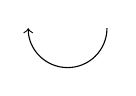
\begin{tikzpicture}[baseline=(A), scale=0.5]
			\coordinate (A) at (0, -0.5);
			\draw[<-] (0, 0) arc[radius=1, start angle=180, end angle=360];
		\end{tikzpicture} \; , \quad
		\mathrm{coev}_X := X \times
		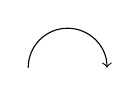
\begin{tikzpicture}[baseline=(A), scale=0.5]
			\coordinate (A) at (0, 0.2);
			\draw[->] (0, 0) arc[radius=1, start angle=180, end angle=0];
		\end{tikzpicture} \; .
	\end{gather*}
	\begin{itemize}
		\item 如前引书, $n\dcate{Cob}$ 的定义已内建双射
		\begin{align*}
			\Hom_{n\dcate{Cob}}(X, Y) & \xleftrightarrow{1:1} \Hom_{n\dcate{Cob}}\left( \emptyset, X^* \sqcup Y\right) \\
			& = \left\{ W: \text{带边定向, 连同资料}\; \partial W \rightiso X^* \sqcup Y \right\} / \sim .
		\end{align*}
		
		\item 态射 (亦即配边) 的对偶无非是将 $\partial W \rightiso X^* \sqcup Y$ 逆转为 $\partial W \rightiso (Y^*)^* \sqcup X^*$.
		
		\item 迹和维数取值在
		\[ \End_{n\dcate{Cob}}(\emptyset) = \left\{ n\;\text{维紧闭流形} \right\}/\sim . \]
		\item 根据先前对 $\mathrm{ev}_X$ 和 $\mathrm{coev}_X$ 的描述, 对 $f \in \End_{n\dcate{Cob}}(X)$ 取迹相当于将配边 $f$ 上下两头的 $X$ 黏合. 由于恒等态射 $\identity_X$ 对应于平凡配边 $X \times [0, 1]$, 故
		\[ \dim X = X \times
		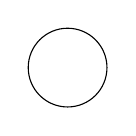
\begin{tikzpicture}[baseline=(O), scale=0.5]
			\coordinate (O) at (0, -0.25);
			\draw (0, 0) circle[radius=1];
		\end{tikzpicture} \; . \]
	\end{itemize}
	
	对于 $n\dcate{Cob}$, 在 \S\ref{sec:monoidal-dual} 引入的各种图解都获得了实际意义. 方法和对象在此具有相同的几何实质.
\end{example}

我们最后来讨论对偶性如何体现于 Hopf 代数上的模和余模; 详见 \S\ref{sec:bialgebra}. 设 $\Bbbk$ 为域, $(A, \mu, \eta, \Delta, \epsilon)$ 为 $\Bbbk$-双代数, 亦即 $\cate{Vect}(\Bbbk)$ 上的双代数. 命题 \ref{prop:bialgebra-Mod-monoidal} 已说明如何同时运用代数和余代数结构赋予下述范畴
\[ A\dcate{Mod}, \quad \cated{Mod}A, \quad A\dcate{Comod}, \quad \cated{Comod}A \]
自然的幺半结构. 我们意欲在其中刻画对偶性. 以下仅就右模和右余模的情形加以阐述.

既然从 $\cated{Mod}A$ (或 $\cated{Comod}A$) 向 $\cate{Vect}(\Bbbk)$ 的忘却函子是幺半函子, 若右 $A$-模 (或 $A$-余模) $M$ 有左或右对偶, 则:
\begin{itemize}
	\item $\dim_{\Bbbk} M < \infty$;
	\item 无论左右, 对偶必然实现在对偶向量空间 $M^\vee := \Hom_{\Bbbk}(M, \Bbbk)$ 上;
	\item $\mathrm{ev}$ 和 $\mathrm{coev}$ 在 $\cate{Vect}_{\mathrm{f}}(\Bbbk)$ 的层次都按例 \ref{eg:Vect-trace} 的方式确定, 精确到同构.
\end{itemize}

如果一个 $A$-模 (或 $A$-余模) 作为 $\Bbbk$-向量空间是有限维的, 则称之为有限维 $A$-模 (或 $A$-余模). 以下便聚焦于有限维的 $M$, 相应的范畴记为 $\catesubd{Mod}{\mathrm{f}}A$ 等\footnote{莫和定理 \ref{prop:identify-ModR-fg} 的 $\catesubd{Mod}{\mathrm{fg}}A$ 混淆, 后者是有限生成右 $A$-模范畴.}. 对于熟悉交换环论的读者, 将后续结论推广到一般的交换环 $\Bbbk$ 是毫不费力的, 前提是要求 $M$ 是有限生成投射 $\Bbbk$-模.
\index[sym1]{Modf@$\cate{Mod}_{\mathrm{f}}$}

关键是赋予 $M^\vee$ 合适的右 $A$-模 (或 $A$-余模) 结构. 记 $\otimes := \otimes_{\Bbbk}$. 有限维情形的对偶函子延拓为
\[ (\cdot)^\vee := \Hom_{\Bbbk}(\cdot, \Bbbk): \cate{Vect}(\Bbbk)^{\opp} \to \cate{Vect}(\Bbbk). \]
它仅是右松的: 存在典范的 $N^\vee \otimes M^\vee \to (M \otimes N)^\vee$. 我们仍有一族求值态射
\[ \mathrm{ev}_M: M \otimes M^\vee \to \Bbbk. \]
先考虑 $M$ 为右 $A$-模的情形, 纯量乘法来自 $a: M \otimes A \to M$. 既然 $\cate{Vect}(\Bbbk)$ 是具体的范畴, 元素和映射的语言更为直白. 按以下方式取转置 ${}^t a: A \otimes M^\vee \to M^\vee$, 可使 $M^\vee$ 成为左 $A$-模:
\[ \mathrm{ev}\left(m, {}^t a(t \otimes \lambda)\right) = \mathrm{ev}\left( a(m \otimes t), \lambda \right), \]
其中 $m \in M$, $\lambda \in M^\vee$, $t \in A$.

对于右 $A$-余模 $M$ 的情形, 我们选定 $M$ 的基 $v_1, \ldots, v_n$ 和 $M^\vee$ 的对偶基 $\check{v}_1, \ldots, \check{v}_n$, 按此描述余模结构为
\begin{equation}\label{eqn:comodule-basis}
	\rho(v_i) = \sum_{j=1}^n v_j \otimes t_{ji}, \quad t_{ji} \in A, \quad 1 \leq i \leq n.
\end{equation}
对于 $\rho$, 先前的转置操作有对偶版本: 命
\[ {}^t \rho: M^\vee \to A \otimes M^\vee, \quad \check{v}_i \mapsto \sum_{j=1}^n t_{ij} \otimes \check{v}_j. \]
从 \eqref{eqn:comodule-matrix} 及其左余模版本可见 ${}^t \rho$ 使 $M^\vee$ 成为左 $A$-余模, 还可以验证此结构无关基的选取.

问题是如何调整回右 $A$-模和右 $A$-余模. 这点在 $A$ 为 Hopf 代数时可以典范地做到. 记述如下.

\begin{proposition}\label{prop:Hopf-module-dual}
	\index{duiou!Hopf 模}
	设 $\Bbbk$ 为域. 设 $A$ 为以 $S$ 为对极的 Hopf $\Bbbk$-代数 (定义 \ref{def:Hopf-algebra}), 资料具体写作 $(A, \mu, \eta, \Delta, \epsilon)$. 设 $M$ 为有限维右 $A$-模 (或 $A$-余模), 则 $M$ 兼有左对偶和右对偶, 都实现在 $M$ 的对偶向量空间 $M^\vee$ 上, 具体描述如下:
	\begin{itemize}
		\item 设右 $A$-模 $M$ 的结构来自 $a: M \otimes A \to M$, 则:
		\begin{center}\begin{tabular}{|c|c|} \hline
			左对偶 & 右对偶 \\ \hline
			${}^\vee a: M^\vee \otimes A \to M^\vee$ & $a^\vee: M^\vee \otimes A \to M^\vee$ \\
			${}^\vee a(\lambda \otimes t) = {}^t a\left( S^{-1} t \otimes \lambda\right)$ & $a^\vee(\lambda \otimes t) = {}^t a\left(St \otimes \lambda \right)$
			\\ \hline
		\end{tabular}\end{center}
		其中 ${}^t a$ 是先前定义的转置, $\lambda \in M^\vee$, $t \in A$ 而 $m \in M$.
		\item 设右 $A$-余模 $M$ 的结构来自 $\rho: M \to M \otimes A$, 选基后具体描述如 \eqref{eqn:comodule-basis}, 则:
		\begin{center}\begin{tabular}{|c|c|} \hline
			左对偶 & 右对偶 \\ \hline
			${}^\vee \rho: M^\vee \to M^\vee \otimes A$ & $\rho^\vee: M^\vee \to M^\vee \otimes A$ \\
			${}^\vee \rho (\check{v}_i) = \sum_j \check{v}_j \otimes St_{ij}$ & $\rho^\vee (\check{v}_i) = \sum_j \check{v}_j \otimes S^{-1} t_{ij}$
			\\ \hline
		\end{tabular}\end{center}
	\end{itemize}
	
	作为推论, 有限维右 $A$-模范畴 $\catesubd{Mod}{\mathrm{f}}A$ (或有限维右 $A$-余模范畴 $\catesubd{Comod}{\mathrm{f}}A$) 既是左刚性的也是右刚性的. 左 $A$-模或余模的情形全然相似, 左右对调即可.
\end{proposition}
\begin{proof}
	先讨论右 $A$-模 $M$ 的情形. 延续先前讨论, 既然 $S$ 给出同态 $A \to A^{\mathrm{op}}_{\mathrm{cop}}$ (命题 \ref{prop:Hopf-antiautomorphism}) 而 $\cate{Vect}(\Bbbk)$ 的辫结构对称, 两种方法都使 $M^\vee$ 成为右 $A$-模. 兹断言相对于 $a^\vee$ 赋予 $M^\vee$ 的右 $A$-模结构, $\mathrm{ev}: M \otimes M^\vee \to \Bbbk$ 是右 $A$-模的同态.
	
	以下直接将 $a$ 和 $a^\vee$ 写作右乘, 按照环论习惯将 $\mu: A \otimes A \to A$ 写作乘法, 并从符号中省略 $\eta: \Bbbk \to A$. 设 $\Delta(t) = \sum_i t_i^{(1)} \otimes t_i^{(2)}$. 让 $t$ 右乘于 $m \otimes \lambda \in M \otimes M^\vee$ 再求值的产物为
	\[ \mathrm{ev}\left( \sum_i m t_i^{(1)}, \lambda t_i^{(2)} \right) = \mathrm{ev}\left( \sum_i m t_i^{(1)} S\left(t_i^{(2)}\right), \lambda \right). \]
	然而对极的定义蕴涵 $\sum_i t_i^{(1)} S\left(t_i^{(2)}\right) = \epsilon(t)$, 故上式简化为 $\epsilon(t)\mathrm{ev}(m \otimes \lambda)$. 因为 $\Bbbk$ 的 $A$-模结构来自 $\epsilon$, 这就说明了 $\mathrm{ev}$ 是右 $A$-模同态.
	
	其次验证 $\mathrm{coev}: \Bbbk \to M^\vee \otimes M$ 是右 $A$-模同态, $M^\vee$ 的右 $A$-模结构仍来自 $a^\vee$. 将 $M^\vee \otimes M$ 等同于 $\End_{\Bbbk}(M)$, 则 $\mathrm{coev}(1) = \identity_M$, 问题遂归结为对所有 $t \in A$ 验证
	\[ \epsilon(t) \cdot \identity_M = \sum_i \left( t_i^{(2)} \;\text{右乘} \right) \circ \identity_M \circ \left( S t_i^{(1)} \;\text{右乘} \right), \]
	亦即证 $\epsilon(t) = \sum_i S\left(t_i^{(1)}\right) t_i^{(2)}$, 这同样归结为对极定义.
	
	综上, $M^\vee$ 对 $a^\vee$ 给出 $M$ 的右对偶, 记为 $M^*$. 左对偶也可以按类似方法处理, 或者归结为以下简单观察: 以 ${}^\vee a$ 使 $M^\vee$ 成为右 $A$-模, 记为 ${}^* M$, 则容易看出前一步构造给出的 $({}^* M)^*$ 回到 $M$ 本身, 这就说明 ${}^* M$ 是 $M$ 的左对偶.
	
	对有限维右余 $A$-模 $M$, 我们采取待定系数法. 设 $M^\vee$ 带有由环 $A$ 上的 $n \times n$ 矩阵 $U = (u_{ij})_{i, j}$ 确定的右余模结构, 刻画为
	\[ \check{v}_i \mapsto \sum_{j=1}^n \check{v}_j \otimes u_{ji}, \quad 1 \leq i \leq n. \]
	使 $U$ 给出右余模的充要条件已经在 \eqref{eqn:comodule-matrix} 列出.
	
	请忆及 $\mathrm{ev}(v_i, \check{v}_j) = \delta_{i, j}$ (Kronecker 的 $\delta$ 符号) 和 $\mathrm{coev}(1) = \sum_i \check{v}_i \otimes v_i$. 按此不难将 $\mathrm{ev}$ 和 $\mathrm{coev}$ 为右 $A$-余模同态的条件写作
	\begin{equation}\label{eqn:Hopf-module-dual-aux}
		\sum_k t_{ki} u_{kj} = \delta_{i, j} = \sum_k u_{ik} t_{jk}.
	\end{equation}
	记 $T = (t_{ij})_{i, j}$, 记其转置矩阵为 ${}^t T$, 则上述条件以矩阵语言改写为
	\[ ({}^t T) U = 1_{n \times n} = U ({}^t T). \]
	故寻求 $M$ 的右对偶相当于求 $({}^t T)^{-1}$. 类似地, 寻求 $M$ 的左对偶相当于求 ${}^t (T^{-1})$. 关于右对偶和左对偶的断言分别化约为验证
	\begin{align*}
		\sum_k t_{ki} S^{-1}(t_{jk}) & = \delta_{i, j} = \sum_k S^{-1} (t_{ki}) t_{jk}, \\
		\sum_k t_{ik} S(t_{kj}) & = \delta_{i, j} = \sum_k S(t_{ik}) t_{kj}.
	\end{align*}

	这是容易的. 由于 $\Delta(t_{ij}) = \sum_k t_{ik} \otimes t_{kj}$, 对极的定义蕴涵第二式的两边同为 $\epsilon(t_{ij}) = \delta_{i, j}$. 对第二式两边同取 $S^{-1}$, 并且注意到 $S$ 保持幺元而倒转乘法, 整理即得第一式. 证毕.
\end{proof}

当 $A$ 非交换时, ${}^t (T^{-1})$ 和 $({}^t T)^{-1}$ 未必相等. 上述论证因而也提示了左和右对偶一般并不相等.

事实上, 之后的推论 \ref{prop:Hopf-vs-dual} 将说明从有限维余模范畴的刚性如何逆推双代数上的 Hopf 结构, 这将涉及一系列的理论准备.

\section{自同态余代数}\label{sec:coend}
自本节开始是面向淡中范畴理论 (见 \S\ref{sec:Tannakian-cat}) 的一系列铺垫, 但涉及的一些工具和思路有更广泛的应用. 主要参考材料是 \cite{Del90}.

设 $\Bbbk$ 是交换环. 对任何范畴 $\mathcal{A}$ 及函子 $\xi: \mathcal{A} \to \Bbbk\dcate{Mod}$, 我们可以考虑函子的自同态 $\Bbbk$-代数 $\End(\xi)$, 它给出一族 $\Bbbk$-线性映射
\[ \End(\xi) \dotimes{\Bbbk} \xi(X) \to \xi(X), \quad X \in \Obj(\mathcal{A}), \]
它们对 $X$ 具有函子性, 或者写作 $\End(\xi) \dotimes{\Bbbk} \xi \to \xi$. 此外 $\End(\xi)$ 对之还是``泛''的: 根据同义反复, 让一个 $\Bbbk$-代数 $E$ 作用在 $\xi$ 上相当于指定代数的同态 $E \to \End(\xi)$, 而由此泛性质可以抽象地推导 $\End(\xi)$ 的乘法结构.

对于我们行将处理的问题而言, 上述构造的对偶版本更实用也更简单, 但有必要考虑取值在 $\cated{Mod}B$ 的函子, 其中 $B$ 是 $\Bbbk$-代数, 按惯例默认非零. 这和范畴论中称为\emph{余端}的抽象构造密切相关, 本章习题另有说明.

\begin{definition}\label{def:cogebra-L-universal}
	\index[sym1]{coHom-coEnd@$\coHom, \coEnd$}
	设 $\Bbbk$ 为交换环, $B$ 为 $\Bbbk$-代数, $\omega_1, \omega_2: \mathcal{A} \to \cated{Mod}B$ 为函子. 考虑 $(B, B)$-双模 $L$ 连同函子之间的态射 $a: \omega_2 \to \omega_1 \dotimes{B} L$, 亦即一族右 $B$-模同态
	\[ a_X: \omega_2(X) \to \omega_1(X) \dotimes{B} L, \quad X \in \Obj(\mathcal{A}), \]
	使得下图对一切 $f \in \Hom_{\mathcal{A}}(X, Y)$ 皆交换:
	\[\begin{tikzcd}
		\omega_2(X) \arrow[r, "a_X"] \arrow[d, "{\omega_2(f)}"'] & \omega_1(X) \dotimes{B} L \arrow[d, "{\omega_1(f) \otimes \identity}"] \\
		\omega_2(Y) \arrow[r, "a_Y"'] & \omega_1(Y) \dotimes{B} L.
	\end{tikzcd}\]

	从资料 $(L, a)$ 到 $(L', a')$ 的态射定义为双模同态 $t: L \to L'$, 条件是使下图恒交换
	\[\begin{tikzcd}
		\omega_2(X) \arrow[r, "{a_X}"] \arrow[rd, "{a'_X}"'] & \omega_1(X) \dotimes{B} L \arrow[d, "{\identity \otimes t}"] \\
		& \omega_1(X) \dotimes{B} L'
 	\end{tikzcd}\]
 	反过来说, 给定资料 $(L, a)$ 和双模同态 $t: L \to L'$, 可按上图确定 $a'$ 连同态射 $t: (L, a) \to (L', a')$.
 
	若全体资料 $(L, a)$ 和态射所成的范畴有始对象, 则记相应的 $(B, B)$-双模为
	\[ \coHom(\omega_1, \omega_2) = \coHom_{\Bbbk}(\omega_1, \omega_2), \]
	并且记相应的态射为 $\lambda: \omega_2 \to \omega_1 \dotimes{B} L$. 另记
	\[ \coEnd(\omega) = \coEnd_{\Bbbk}(\omega) := \coHom(\omega, \omega). \]
\end{definition}

符号 $\coHom$ 代表 $\operatorname{coHom}$ 而 $\coEnd$ 代表 $\operatorname{coEnd}$, 应设想为 $\Hom$ 和 $\End$ 的对偶, 缩写仅是排版考量. 留意到 $(B, B)$-双模的概念不只依赖 $B$ 的环结构, 还依赖 $\Bbbk$.

\begin{remark}
	观察到 $\coHom(\omega_1, \omega_2) = 0$ 相当于说任何态射 $\omega_2 \to \omega_1 \dotimes{B} L$ 皆为零, 定义并不排除这种可能. 相对于此, 在 $\coEnd(\omega)$ 存在的前提下, 若 $\omega$ 不是常值零函子, 则 $\coEnd(\omega) \neq 0$, 这是因为 $\omega \rightiso \omega \dotimes{B} B$.
\end{remark}

若 $\coEnd(\omega)$ 存在, 对 $\omega \rightiso \omega \dotimes{B} B$ 应用泛性质可得双模同态
\[ \epsilon: \coEnd(\omega) \to B. \]

另一方面, 在所论的 $\coHom$ 存在的前提下, 对 $\omega_1, \omega_2, \omega_3$ 连续操作可得态射
\begin{equation*}
	\omega_3 \to \omega_2 \dotimes{B} \coHom(\omega_2, \omega_3) \to \omega_1 \dotimes{B} \coHom(\omega_1, \omega_2) \dotimes{B} \coHom(\omega_2, \omega_3),
\end{equation*}
泛性质继而给出典范的双模同态
\begin{equation}\label{eqn:L-comult-prep}
	\coHom(\omega_1, \omega_3) \to \coHom(\omega_1, \omega_2) \dotimes{B} \coHom(\omega_2, \omega_3).
\end{equation}

对函子 $\omega_1, \ldots, \omega_4$ 操练例行的论证, 可见 \eqref{eqn:L-comult-prep} 服从余结合律; 这使得 $\coEnd(\omega)$ 在 $(B, B)\dcate{Mod}$ 中成为以 $\epsilon: \coEnd(\omega) \to B$ 为余幺元的余代数, 而每个 $\omega(X)$ 都通过典范态射 $\lambda$ 成为 $\coEnd(\omega)$-余模. 相关讨论总结如下.

\begin{definition-proposition}[自同态余代数]\label{def:cogebra-L}
	\index{zitongtaiyudaishu@自同态余代数 (endomorphism coalgebra)}
	取函子 $\omega: \mathcal{A} \to \cated{Mod}B$, 并且假定 $\coEnd(\omega)$ 存在.
	\begin{itemize}
		\item 作为幺半范畴 $(B, B)\dcate{Mod}$ 的对象, $\coEnd(\omega)$ 具有典范的余代数结构, 使得每个 $\omega(X)$ 通过典范态射成为 $\coEnd(\omega)$-余模, 而且 $\mathcal{A}$ 的态射诱导余模同态. 我们称 $\coEnd(\omega)$ 是 $\omega$ 的自同态余代数\footnote{或者更应该称为余自同态余代数.}.
		\item 对于 $(B, B)\dcate{Mod}$ 中的任意余代数 $L$, 为每个 $\omega(X)$ 相容地指定 $L$-余模结构相当于指定余代数的同态 $\coEnd(\omega) \to L$.
	\end{itemize}
\end{definition-proposition}

\begin{remark}\label{rem:L-cogebra-functoriality}
	给定函子 $T: \mathcal{A}' \to \mathcal{A}$ 和 $\omega_1, \omega_2: \mathcal{A} \to \cated{Mod}B$, 在所论的 $\coHom$ 存在的前提下, 从 $\omega_1(TX) \to \omega_2(TX) \dotimes{B} \coHom(\omega_1, \omega_2)$ 和泛性质自然地诱导出同态
	\[ \coHom(\omega_1 T, \omega_2 T) \to \coHom(\omega_1, \omega_2), \]
	它兼容上述一切结构; 特别地, 取 $\omega_1 = \omega = \omega_2$ 给出余代数同态 $\coEnd(\omega T) \to \coEnd(\omega)$.
\end{remark}

\begin{proposition}\label{prop:coHom-colim}
	取定函子 $\omega_1, \omega_2: \mathcal{A} \to \cated{Mod}B$. 设 $\mathcal{A}$ 是一族子范畴的并, 将这些子范畴记为 $\mathcal{A}'$ 的形式, 并且记 $\omega'_i := \omega_i|_{\mathcal{A}'}$. 假设 $\coHom(\omega'_1, \omega'_2)$ 对所有 $\mathcal{A}'$ 皆存在, 则 $\coHom(\omega_1, \omega_2)$ 存在, 并且有典范同构
	\[ \varinjlim_{\mathcal{A}'} \coHom(\omega'_1, \omega'_2) \rightiso \coHom(\omega_1, \omega_2); \]
	左侧的 $\varinjlim$ 按包含关系赋序, 转移同态由注记 \ref{rem:L-cogebra-functoriality} 的方式给出. 同构兼容于 \eqref{eqn:L-comult-prep}.
\end{proposition}
\begin{proof}
	对任意 $(B, B)$-双模 $L$, 指定 $\omega_2 \to \omega_1 \dotimes{B} L$ 相当于对所有 $\mathcal{A}'$ 指定 $\omega'_2 \to \omega'_1 \dotimes{B} L$, 要求彼此兼容; 这也相当于给定一族兼容的同态 $\coHom(\omega'_1, \omega'_2) \to L$.
\end{proof}

问题在于如何确保 $\coHom(\omega_1, \omega_2)$ 存在, 这不尽然是平凡的. 首先须控制范畴的大小. 选定 Grothendieck 宇宙 $\mathcal{U}$, 依此可以谈论何谓小集和小范畴. 若一个范畴的所有对象的同构类形成一个小集, 则称该范畴为本质小的 (定义 \ref{def:essentially-small-cat}).

\begin{convention}\label{con:Mod-pfg}
	\index[sym1]{Modpfg@$\cate{Mod}_{\mathrm{pfg}}$}
	选定交换环 $\Bbbk$ 和 $\Bbbk$-代数 $B$. 我们需要一系列的符号.
	\begin{itemize}
		\item 考虑全子范畴
		\[ \underbracket{\catesubd{Mod}{\mathrm{pfg}}B}_{\text{投射 + 有限生成}} \subset \underbracket{\catesubd{Mod}{\mathrm{fg}}B}_{\text{有限生成}} \subset \cated{Mod}B. \]
		\item 对任意右 $B$-模 $P$, 按 \eqref{eqn:P-vee} 定义左 $B$-模 $P^\vee$. 任何同态 $\varphi: P \to Q$ 皆诱导对偶同态 $\varphi^\vee: Q^\vee \to P^\vee$.
	\end{itemize}
	根据本书关于代数结构的惯例, 默认 $\Bbbk$ 和 $B$ 实现在小集上. 基于有限生成的条件, $\catesubd{Mod}{\mathrm{fg}}B$ 和 $\cate{Vect}_{\mathrm{f}}(\Bbbk)$ 都是本质小范畴, 它们还都是 $\Bbbk$-线性的. 然而本节考虑的本质小范畴 $\mathcal{A}$ 不要求有 $\Bbbk$-线性结构.
\end{convention}

对所有 $P_1, P_2 \in \Obj(\catesubd{Mod}{\mathrm{pfg}}B)$, 我们有典范同构
\begin{equation*}\begin{aligned}
	\Hom_{\cated{Mod}B}\left( P_2, P_1 \dotimes{B} L \right) & \rightiso \Hom_{(B, B)\dcate{Mod}}\left( P_1^\vee \dotimes{\Bbbk} P_2, L \right) \\
	\varphi & \mapsto \left[ \check{p}_1 \otimes p_2 \mapsto (\check{p}_1 \otimes \identity_L)(\varphi(p_2)) \right] ;
\end{aligned}\end{equation*}
这很容易化约到 $P_1$ 和 $P_2$ 是有限秩自由模的情形来验证. 由此可见当 $\omega_1, \omega_2: \mathcal{A} \to \cated{Mod}B$ 取值在 $\catesubd{Mod}{\mathrm{pfg}}B$ 时, 指定定义 \ref{def:cogebra-L-universal} 述及的资料 $a = (a_X)_X$ 等价于指定一族同态
\[ \alpha_X: \omega_1(X)^\vee \dotimes{\Bbbk} \omega_2(X) \to L, \quad X \in \Obj(\mathcal{A}), \]
它们对 $X$ 的函子性翻译如下: 对所有 $f \in \Hom_{\mathcal{A}}(X, Y)$, 下图交换.
\begin{equation}\label{eqn:cogebra-L}\begin{tikzcd}
	\omega_1(Y)^\vee \dotimes{\Bbbk} \omega_2(X) \arrow[r, "{\omega_1(f)^\vee \otimes \identity}" inner sep=0.6em] \arrow[d, "{\identity \otimes \omega_2(f)}"'] & \omega_1(X)^\vee \dotimes{\Bbbk} \omega_2(X) \arrow[d, "{\alpha_X}"] \\
	\omega_1(Y)^\vee \dotimes{\Bbbk} \omega_2(Y) \arrow[r, "{\alpha_Y}"'] & L.
\end{tikzcd}\end{equation}

\begin{proposition}\label{prop:cogebra-L-universal}
	设 $\mathcal{A}$ 为本质小范畴, $\omega_1, \omega_2: \mathcal{A} \to \catesubd{Mod}{\mathrm{pfg}}B$ 为任意函子, 则定义 \ref{def:cogebra-L-universal} 中的 $\coHom(\omega_1, \omega_2)$ 存在.
\end{proposition}
\begin{proof}
	唯一待说明的是始对象的存在性. 关键是应用交换图表 \eqref{eqn:cogebra-L}. 取 $L_0$ 为所有 $\omega_1^\vee(X) \dotimes{\Bbbk} \omega_2(X)$ 的直和, 其中 $X$ 遍历 $\Obj(\mathcal{A})/\simeq$ 的一族代表元; 此处需要本质小的条件. 接着对所有 $f: X \to Y$ 定义
	\[ \delta_f := \omega_1(f)^\vee \otimes \identity - \identity \otimes \omega_2(f) : \omega_1(Y)^\vee \dotimes{\Bbbk} \omega_2(X) \to L_0. \]
	取 $\coHom(\omega_1, \omega_2) := L_0 / \sum_f \Image(\delta_f)$ 即所求.
\end{proof}

\begin{convention}\label{con:coend-bracket}
	以下的具体表法是方便的: 对 $t \in \omega_1(X)^\vee \dotimes{\Bbbk} \omega_2(X)$, 它在 $\coHom(\omega_1, \omega_2)$ 中的像记为 $[t]$; 这些像生成 $\coHom(\omega_1, \omega_2)$. 在定义 \ref{def:cogebra-L} 的泛性质中, $[\phi \otimes x] \in \coEnd(\omega)$ 在 $L$ 中的像是先取 $x \in \omega(X)$ 对 $\omega(X) \to \omega(X) \dotimes{B} L$ 的像, 再用 $\phi \in \omega(X)^\vee$ 缩并的产物.
\end{convention}

对函子 $\omega: \mathcal{A} \to \catesubd{Mod}{\mathrm{pfg}}B$, 求值同态 $\mathrm{ev}_{\omega(X)}: \omega(X)^\vee \dotimes{\Bbbk} \omega(X) \to B$ 是 $(B, B)$-双模同态, 它确定的典范同态正是先前定义的
\begin{equation}\label{eqn:L-counit}
	\begin{aligned}
		\epsilon: \coEnd(\omega) & \to B \\
		[t] & \mapsto \mathrm{ev}_{\omega(X)}(t).
	\end{aligned}
\end{equation}

当 $\omega_1(X)$ 自由时, 取其 $B$-基 $(v_i)_{i=1}^n$ 和对偶基 $(\check{v}_i)_{i=1}^n$, 则 $\lambda_X: \omega_2(X) \to \omega_1(X) \dotimes{B} \coHom(\omega_1, \omega_2)$ 可以表作
\begin{equation}\label{eqn:L-coaction}\begin{aligned}
	w & \mapsto \sum_{i=1}^n v_i \otimes [\check{v}_i \otimes w];
\end{aligned}\end{equation}
基于此, 对任意 $\omega_1, \omega_2, \omega_3$, 在 $\omega_1(X)$ 和 $\omega_2(X)$ 自由, $\lambda \in \omega_1(X)^\vee$ 和 $w \in \omega_3(X)$ 的前提下推得
\begin{equation}\label{eqn:L-comult}\begin{aligned}
	\coHom(\omega_1, \omega_3) & \to \coHom(\omega_1, \omega_2) \dotimes{B} \coHom(\omega_2, \omega_3) \\
	[\lambda \otimes w] & \mapsto \sum_i [\lambda \otimes v_i] \otimes [\check{v}_i \otimes w].
\end{aligned}\end{equation}

下一步是引进幺半结构. 为此必须要求 $B$ 交换, 并且在前述构造中取 $\Bbbk = B$. 于是 $\cated{Mod}B$ 和 $\catesubd{Mod}{\mathrm{pfg}}B$ 对 $\otimes_B$ 皆是对称幺半范畴, 以 $B$ 为幺元. 我们将对应的 $\coHom$ 和 $\coEnd$ 标为 $\coHom_B$ 和 $\coEnd_B$ 以资强调; 此时 $(B, B)$-双模和 $B$-模是一回事.

取 $\mathcal{A}$, $\mathcal{A}'$ 等为任意范畴. 首先给定函子
\[ \omega_i: \mathcal{A} \to \cated{Mod}B, \quad \omega'_i: \mathcal{A}' \to \cated{Mod}B, \quad i =1, 2. \]
定义 $\omega_i \boxtimes \omega'_i: \mathcal{A} \times \mathcal{A}' \to \cated{Mod}B$, 映对象 $(X, X')$ 为 $\omega_i(X) \dotimes{B} \omega'_i(X')$.

在所论 $\coHom$ 存在的前提下, 对态射族
\begin{align*}
	\omega_2(X) \dotimes{B} \omega'_2(X') & \to \omega_1(X) \dotimes{B} \coHom_B(\omega_1, \omega_2) \dotimes{B} \omega'_1(X') \dotimes{B} \coHom_B(\omega'_1, \omega'_2) \\
	& \simeq \omega_1(X) \dotimes{B} \omega'_1(X') \dotimes{B} \coHom(\omega_1, \omega_2) \dotimes{B} \coHom_B(\omega'_1, \omega'_2)
\end{align*}
应用泛性质, 可得典范态射
\[ \nu: \coHom_B(\omega_1 \boxtimes \omega'_1, \omega_2 \boxtimes \omega'_2) \to \coHom_B(\omega_1, \omega_2) \dotimes{B} \coHom_B(\omega'_1, \omega'_2), \]
它使下图对所有 $(X, X') \in \Obj(\mathcal{A} \times \mathcal{A}')$ 交换:
\[\begin{tikzpicture}
	\node (A) {$\omega_2(X) \dotimes{B} \omega'_2(X')$};
	\node (B) [right=of A] {$\omega_1(X) \dotimes{B} \omega'_1(X') \dotimes{B} \coHom_B(\omega_1 \boxtimes \omega'_1, \omega'_2 \boxtimes \omega'_2)$};
	\node (C) [below=of B] {$\omega_1(X) \dotimes{B} \omega'_1(X') \dotimes{B} \coHom_B(\omega_1, \omega_2) \dotimes{B} \coHom_B(\omega'_1, \omega'_2)$.};
	
	\draw[->] (A) -- (B) node[midway, above] {\scriptsize 典范};
	\draw[->] (A) -- (C.north west) node[midway, below left] {\scriptsize 典范};
	\draw[->] (B) -- (C) node[midway, auto] {\scriptsize $\identity \otimes \identity \otimes \nu$};
\end{tikzpicture}\]

\begin{lemma}
	符号如上, 并且设 $\omega_i$ 和 $\omega'_i$ 皆取值在 $\catesubd{Mod}{\mathrm{pfg}}B$, 则 $\omega_i \boxtimes \omega'_i$ 亦然, 而且此时 $\nu$ 是同构; 它可以按照约定 \ref{con:coend-bracket} 具体描述为
	\begin{equation*}
		\nu: \left[ (\phi \otimes \phi') \otimes (x \otimes x') \right] \mapsto [\phi \otimes x] \otimes [\phi' \otimes x'].
	\end{equation*}
\end{lemma}
\begin{proof}
	既然 $\catesubd{Mod}{\mathrm{pfg}}B$ 对 $\otimes_B$ 封闭, 故 $\omega \boxtimes \omega'$ 取值在其中. 回归 \eqref{eqn:cogebra-L} 和命题 \ref{prop:cogebra-L-universal} 的构造即可验证 $\nu$ 的具体描述.
	
	接着说明 $\nu$ 为同构. 按照命题 \ref{prop:cogebra-L-universal} 的构造, $\coHom_B(\omega_1, \omega_2)$ 可以适当地表成 $\varinjlim_{X, Y} \omega_1(Y)^\vee \dotimes{B} \omega_2(X)$, 相关态射来自 \eqref{eqn:cogebra-L}; 对于 $\nu$ 涉及的其他 $\coHom_B$ 自然也是如此. 因此, 说 $\nu$ 为同构相当于说自明的态射
	\begin{multline*}
		\varinjlim_{X, X', Y, Y'} \omega_1(Y)^\vee \dotimes{B} \omega'_1(Y')^\vee \dotimes{B} \omega_2(Y) \dotimes{B} \omega'_2(Y') \\
		\to \varinjlim_{X, Y} \left( \omega_1(Y)^\vee \dotimes{B} \omega_2(X) \right) \dotimes{B} \varinjlim_{X', Y'} \left( \omega'_1(Y')^\vee \dotimes{B} \omega'_2(X') \right)
	\end{multline*}
	为同构, 而这又归结为关于 $\dotimes{B}$ 保小 $\varinjlim$ 的模论常识 \cite[命题 6.9.2]{Li1}.
\end{proof}

继续先前的讨论. 考虑函子
\begin{gather*}
	\otimes: \mathcal{A} \times \mathcal{A}' \to \mathcal{A}'' , \\
	\omega_i: \mathcal{A} \to \catesubd{Mod}{\mathrm{pfg}}B, \quad \omega'_i: \mathcal{A}' \to \catesubd{Mod}{\mathrm{pfg}}B, \quad \omega''_i: \mathcal{A}'' \to \catesubd{Mod}{\mathrm{pfg}}B \quad i =1, 2,
\end{gather*}
连同同构 $\theta_i: \omega_i \boxtimes \omega'_i \rightiso \omega''_i \circ \otimes$, 其对偶版本记为 $\theta_i^\vee$; 前一段铺垫给出 $B$-线性的同态
\begin{equation}\label{eqn:L-tensor}
	\begin{tikzcd}[row sep=tiny, column sep=small]
		\coHom_B(\omega_1, \omega_2) \dotimes{B} \coHom_B(\omega'_1, \omega'_2) \arrow[r, "{\nu^{-1}}", "{\theta_1, \theta_2}"' inner sep=0.6em] & \coHom_B(\omega''_1 \circ \otimes, \; \omega''_2 \circ \otimes) \arrow[r, "{\text{注记 \ref{rem:L-cogebra-functoriality}}}" inner sep=0.6em] & \coHom_B(\omega''_1, \omega''_2) \\
		{[\phi \otimes x]} \otimes {[\phi' \otimes x']} \arrow[mapsto, rr] & & {\left[ \theta_1^\vee(\phi \otimes \phi'), \theta_2(x \otimes x') \right]} .
	\end{tikzcd}
\end{equation}
先前关于 $\nu$ 的交换图表蕴涵下图交换, 细节留给读者.
\begin{equation}\label{eqn:L-bialgebra-prod}
	\begin{tikzcd}[row sep=small, column sep=small]
		\omega''_2(X \otimes X') \arrow[d, "{\theta_2^{-1}}", "\sim"' sloped] \arrow[r, "\text{典范}"] & \omega''_1(X \otimes X') \dotimes{B} \coHom_B(\omega''_1, \omega''_2) \\
		\omega_2(X) \dotimes{B} \omega'_2(X') \arrow[d, "\text{典范}" inner sep=0.6em] &  \\
		\omega_1(X) \dotimes{B} \omega'_1(X') \dotimes{B} \coHom_B(\omega_1, \omega_2) \dotimes{B} \coHom_B(\omega'_1, \omega'_2) \arrow[r, "\text{\eqref{eqn:L-tensor}}"' inner sep=0.6em] & \omega_1(X) \dotimes{B} \omega'_1(X') \dotimes{B} \coHom_B(\omega''_1, \omega''_2). \arrow[uu, "{\theta_1 \otimes \identity}"', "\sim" sloped]
	\end{tikzcd}
\end{equation}

现在进一步假设 $\mathcal{A} = \mathcal{A}' = \mathcal{A}''$ 是幺半范畴, $\otimes$ 为其乘法, $\omega''_i = \omega'_i = \omega_i$ 是幺半函子 ($i=1,2$). 记 $\mathcal{A}_0$ 为仅有一个对象和一个态射 (即恒等) 的范畴, $\iota: \mathcal{A}_0 \to \mathcal{A}$ 映唯一对象为 $\munit$. 简单操演定义可见
\[ \coHom_B(\omega_1 \iota, \omega_2 \iota) \simeq B \dotimes{B} B \simeq B. \]
注记 \ref{rem:L-cogebra-functoriality} 的函子性遂给出典范映射
\begin{equation}\label{eqn:L-bialgebra-unit}
	B \simeq \coHom_B(\omega_1 \iota, \omega_2 \iota) \to \coHom_B(\omega_1, \omega_2), \quad b \mapsto [b \otimes 1] = [1 \otimes b].
\end{equation}

\begin{proposition}\label{prop:L-bialgebra}
	在上述场景中取 $\mathcal{A} = \mathcal{A}' = \mathcal{A}''$ 为幺半范畴, $\omega_1$ 和 $\omega_2$ 为幺半函子, $\omega''_i = \omega'_i = \omega_i$.
	\begin{enumerate}[(i)]
		\item 相应的同态 $\coHom_B(\omega_1, \omega_2) \dotimes{B} \coHom_B(\omega_1, \omega_2) \to \coHom_B(\omega_1, \omega_2)$ 使 $\coHom_B(\omega_1, \omega_2)$ 成为 $B$-代数, 以 \eqref{eqn:L-bialgebra-unit} 为幺元.
		\item 对于特例 $\omega_1 = \omega = \omega_2$, 这使 $\coEnd_B(\omega)$ 成为双代数.
		\item 若 $\mathcal{A}$ 是对称幺半范畴, $\omega_1$ 和 $\omega_2$ 兼容辫结构, 则 $\coHom_B(\omega_1, \omega_2)$ 是交换 $B$-代数.
	\end{enumerate}
\end{proposition}
\begin{proof}
	由于乘法 $\coHom_B(\omega_1, \omega_2)$ 有基于 \eqref{eqn:L-tensor} 和 \eqref{eqn:L-bialgebra-prod} 的自然刻画, 其余一切都是幺半结构的反映, 所需只是形式论证, 此处略去.
\end{proof}

\section{重构定理}\label{sec:Tannaka-coend}
本节选定交换环 $\Bbbk$. 除非另外说明, 以下考虑的范畴和函子都是 $\Bbbk$-线性的; 特别地, 幺半范畴的双函子 $\otimes$ 对每个变元都默认为 $\Bbbk$-线性的. 约定 \ref{con:Mod-pfg} 已经对 $\Bbbk$-代数 $B$ 定义了本质小范畴 $\catesubd{Mod}{\mathrm{pfg}}B \subset \catesubd{Mod}{\mathrm{fg}}B$. 对于幺半范畴 $(B, B)\dcate{Mod}$ 中的余代数 $C$, 记 $\cated{Comod}C$ 为 $C$ 的右余模范畴, 这些余模是叠架在 $\cated{Mod}B$ 上的结构, 详见定义 \ref{def:cogebroid} 的说明. 施加作为右 $B$-模的投射性/有限性条件, 便有全子范畴
\[ \underbracket{\catesubd{Comod}{\mathrm{pf}}C}_{\text{投射 + 有限生成}} \subset \underbracket{\catesubd{Comod}{\mathrm{f}}C}_{\text{有限生成}} \subset \cated{Comod}C. \]
\index[sym1]{Comodpfg@$\cate{Comod}_{\mathrm{pf}}, \cate{Comod}_{\mathrm{f}}$}

基于有限生成的条件, $\catesubd{Comod}{\mathrm{f}}C$ 仍是定义 \ref{def:essentially-small-cat} 所谓的本质小范畴.

为了对 \S\ref{sec:coend} 介绍的 $\coEnd(\omega) = \coEnd_{\Bbbk}(\omega)$ 有更具体的把握, 现在切入命题 \ref{prop:Morita-comonad} 的场景: 考虑 $\Bbbk$-代数 $A$, $B$ (未必交换) 和 $(A, B)$-双模 $P$, 并且设 $P$ 是有限生成投射右 $B$-模. 取 $\mathcal{A}$ 为 $\cated{Mod}A$ 的全子范畴, 使得
\begin{itemize}
	\item $A \in \Obj(\mathcal{A})$,
	\item $\omega := (\cdot) \dotimes{A} P$ 给出函子 $\mathcal{A} \to \catesubd{Mod}{\mathrm{pfg}}B$.
\end{itemize}

命题 \ref{prop:Morita-comonad} 断言 $(B, B)$-双模 $P^\vee \dotimes{A} P$ 是余代数, 对应到伴随对
\begin{equation*}\begin{tikzcd}
	(\cdot) \dotimes{A} P : \cated{Mod}A \arrow[shift left, r] & \cated{Mod}B: (\cdot) \dotimes{B} P^\vee \arrow[shift left, l]
\end{tikzcd}\end{equation*}
所确定的余单子: $P^\vee \dotimes{A} P$ 自然地余作用于每个 $\omega(N) = N \dotimes{A} P$. 精确地说, 余作用是
\[ N \dotimes{A} P \xrightarrow{\identity_N \otimes \mathrm{coev} \otimes \identity_P} N \dotimes{A} P \dotimes{B} P^\vee \dotimes{A} P, \quad N \in \Obj(A\dcate{Mod}). \]

定义--命题 \ref{def:cogebra-L} 遂给出余代数的典范同态
\[ \coEnd(\omega) \to P^\vee \dotimes{A} P. \]

\begin{proposition}\label{prop:endomorphism-vs-P}
	在上述情境中, $\coEnd(\omega) \to P^\vee \dotimes{A} P$ 是同构.
\end{proposition}
\begin{proof}
	取 $\cated{Mod}A$ 的全子范畴 $\mathcal{A}^\flat$ 使得 $\Obj(\mathcal{A}^\flat) = \{A\}$, 相应的包含函子记为 $i$. 注记 \ref{rem:L-cogebra-functoriality} 给出交换图表
	\[\begin{tikzcd}[column sep=tiny]
		\coEnd(\omega i) \arrow[rr] \arrow[rd] & & \coEnd(\omega), \arrow[ld] \\
		& P^\vee \dotimes{A} P & 
	\end{tikzcd}\]
	请读者简单地验证 $\coEnd(\omega i) \rightiso P^\vee \dotimes{A} P$. 于是 $\coEnd(\omega i) \to \coEnd(\omega)$ 有左逆; 若能证明它满, 则 $\coEnd(\omega i) \rightiso \coEnd(\omega)$, 从而 $\coEnd(\omega) \rightiso P^\vee \dotimes{A} P$.
	
	基于 $\coEnd(\omega)$ 和 $\coEnd(\omega i)$ 的具体构造, 问题化为对所有 $Y \in \Obj(\mathcal{A})$ 证明
	\[ \Image\left[ \omega(Y)^\vee \dotimes{\Bbbk} \omega(Y) \to \coEnd(\omega) \right] \subset \Image\left[ \omega(A)^\vee \dotimes{\Bbbk} \omega(A) \to \coEnd(\omega) \right]. \]
	
	将任意 $t \in \omega(Y)^\vee \dotimes{\Bbbk} \omega(Y)$ 写作有限和 $\sum_i \lambda_i \otimes o_i$; 基于 $\omega$ 的具体取法, 每个 $o_i \in \omega(Y)$ 又可以表作形如 $\omega(f)(x)$ 的元素的有限线性组合, 其中 $x \in \omega(A)$ 而 $f \in \Hom_{\mathcal{A}}(A, Y)$. 于是问题进一步化到 $t = \lambda \otimes \omega(f)(x)$ 的情形. 然而这点可以通过在交换图表
	\[\begin{tikzcd}
		\omega(Y)^\vee \dotimes{\Bbbk} \omega(A) \arrow[r, "{\omega(f)^\vee \otimes \identity}" inner sep=0.6em] \arrow[d, "{\identity \otimes \omega(f)}"'] & \omega(A)^\vee \dotimes{\Bbbk} \omega(A) \arrow[d] \\
		\omega(Y)^\vee \dotimes{\Bbbk}  \omega(Y) \arrow[r] & \coEnd(\omega)
	\end{tikzcd}\]
	中考虑 $\lambda \otimes x \in \omega(Y)^\vee \dotimes{\Bbbk} \omega(A)$ 的像来说明.
\end{proof}

对于任何本质小范畴 $\mathcal{A}$ 和函子 $\omega: \mathcal{A} \to \catesubd{Mod}{\mathrm{pfg}}B$, 定义--命题 \ref{def:cogebra-L} 将 $\omega$ 典范地分解为
\begin{equation}\label{eqn:L-canonical-decomp}
	\mathcal{A} \xrightarrow{\overline{\omega}} \catesubd{Comod}{\mathrm{pf}}\coEnd(\omega) \xrightarrow{U} \catesubd{Mod}{\mathrm{pfg}}B,
\end{equation}
其中 $U$ 是忘却函子. 我们希望探究 $\overline{\omega}$ 何时为等价.

以下引理将为之后的种种重构定理奠定基础, 证明主干基于 Beck 单子性定理 \ref{prop:Beck}. 我们也将需要命题 \ref{prop:faithful-exact} 对忠实正合函子的刻画, 定义 \ref{def:locally-finite} 关于局部有限 Abel 范畴的概念, 以及\CHref{sec:app-Ind}关于 $\Ind$ 化的一点技巧.

\begin{lemma}\label{prop:Tannaka-projective-generator}
	设 $\Bbbk$ 为域, $\mathcal{A}$ 是局部有限 Abel 范畴, $s$ 是 $\mathcal{A}$ 的投射生成元. 考虑忠实正合函子
	\[ \omega: \mathcal{A} \to \cated{Mod}B, \]
	并假设它取值在 $\catesubd{Mod}{\mathrm{pfg}}B$ 中.
	\begin{enumerate}[(i)]
		\item 余代数 $\coEnd(\omega)$ 可以具体表作 $P^\vee \dotimes{A} P$, 其中 $A = \End_{\mathcal{A}}(s)$ 而 $P = \omega(s)$.
		\item 典范分解 \eqref{eqn:L-canonical-decomp} 中的 $\overline{\omega}$ 是范畴等价.
		\item 我们有 $\catesubd{Comod}{\mathrm{pf}}\coEnd(\omega) = \catesubd{Comod}{\mathrm{f}}\coEnd(\omega)$.
	\end{enumerate}
\end{lemma}
\begin{proof}
	观察到 $A$ 是有限维 $\Bbbk$-代数. 此时定理 \ref{prop:identify-ModR-fg} 的前提全部成立, $\Hom_{\mathcal{A}}(s, \cdot)$ 给出等价 $\mathcal{A} \to \catesubd{Mod}{\mathrm{fg}}A$. 问题依此化约到 $\mathcal{A} = \catesubd{Mod}{\mathrm{fg}}A$ 而 $s = A$ 的情形. 第一个观察是 $\omega$ 此时典范地延拓为函子
	\[ \Omega: \cated{Mod}A \to \cated{Mod}B , \]
	具体方法是:
	\begin{description}
		\item[对象层次] 取滤过小 $\varinjlim$
		\begin{equation}\label{eqn:Tannaka-tilde-omega}
			\Omega(N) = \varinjlim_{\substack{N' \subset N \\ \text{有限生成}}} \omega(N');
		\end{equation}
		\item [态射层次] 对右 $A$-模的同态 $f: N_1 \to N_2$ 取
		\begin{align*}
			\Omega(f) & = \varprojlim_{N'_1 \subset N_1} \varinjlim_{\substack{N'_2 \subset N_2 \\ N'_2 \supset \Image\omega(f|_{N'_1}) }} \left[ \omega(f|_{N'_1}): \omega(N'_1) \to \omega(N'_2) \right] \\
			& \in \varprojlim_{N'_1 \subset N_1} \varinjlim_{N'_2 \subset N_2} \Hom_{\cated{Mod}B}\left( \omega(N'_1), \omega(N'_2)\right),
		\end{align*}
		右式按显然的方式确定从 $\Omega(N_1)$ 到 $\Omega(N_2)$ 的同态.
	\end{description}

	倘若读者愿意调用 \S\S\ref{sec:ind-pro}---\ref{sec:Indization} 关于 $\IndC$ 化的理论, 则这不外是将 $\cated{Mod}A$ 等同于 $\IndC\left( \catesubd{Mod}{\mathrm{fg}}A \right)$, 然后应用 $\cated{Mod}B$ 的余完备性质, 将函子 $\omega$ 依照滤过 $\varinjlim$ 延拓到  $\IndC\left( \catesubd{Mod}{\mathrm{fg}}A \right)$ 上的结果, 详见定义--命题 \ref{def:Ind-hat-functor}.
	
	下列性质既是关于 $\IndC$ 化的一般事实, 也可以直接从 $\Omega$ 的构造来检验.
	\begin{itemize}
		\item $\Omega$ 在 $\catesubd{Mod}{\mathrm{fg}}A$ 上的限制同构于 $\omega$.
		\item $\Omega$ 是正合 $\Bbbk$-线性函子 --- 见命题 \ref{prop:Ind-ext-exactness} (ii) 及其上的讨论, 用到 $\omega$ 的正合性, 以及 $\cated{Mod}B$ 是 Grothendieck 范畴这一事实.
		\item $\Omega$ 保持所有小 $\varinjlim$ --- 见命题 \ref{prop:Ind-ext-exactness} (iii), 用到 $\catesubd{Mod}{\mathrm{fg}}A$ 本质小这一事实.
	\end{itemize}

	此外, $\omega$ 左正合蕴涵对于 $N$ 的所有有限生成子模 $N' \subset N''$, 在 \eqref{eqn:Tannaka-tilde-omega} 中的转移同态 $\omega(N') \to \omega(N'')$ 皆单, 故滤过 $\varinjlim$ 在模范畴中的初等构造表明
	\[ \Omega(N) = 0 \iff \forall N', \; \omega(N') = 0 \stackrel{\because \;\omega\;\text{忠实}}{\iff} \; \forall N', \; N' = 0 \iff N = 0. \]
	综上可见 $\Omega$ 忠实正合.
		
	现在可以对函子 $\Omega$ 应用定理 \ref{prop:Morita} 以得出
	\[ \Omega \simeq (\cdot) \dotimes{A} P, \quad P := \Omega(A) = \omega(A) \in \Obj(\catesubd{Mod}{\mathrm{pfg}}B). \]
	它限制到 $\catesubd{Mod}{\mathrm{fg}}A$ 给出原函子 $\omega$; 鉴于命题 \ref{prop:endomorphism-vs-P}, 这也一并给出 (i) 对 $\coEnd(\omega)$ 的描述.
	
	既然 $\Omega$ 忠实正合, 命题 \ref{prop:Morita-descent} 蕴涵伴随对
	\begin{equation*}\begin{tikzcd}
			(\cdot) \dotimes{A} P : \cated{Mod}A \arrow[shift left, r] & \cated{Mod}B: (\cdot) \dotimes{B} P^\vee \arrow[shift left, l]
	\end{tikzcd}\end{equation*}
	是余单子的, 相应的余代数是先前见过的 $P^\vee \dotimes{A} P$. 综之, $\Omega$ 典范地分解为等价和忘却:
	\[ \cated{Mod}A \xrightarrow[\sim]{\overline{\Omega}} \cated{Comod}\left(P^\vee \dotimes{A} P\right) \xrightarrow{U} \cated{Mod}B. \]
	
	基于命题 \ref{prop:Morita-comonad-ft}, 上述分解限制为交换图表
	\[\begin{tikzcd}
		\catesubd{Mod}{\mathrm{fg}}A \arrow[r, "\sim"'] \arrow[rd, bend right] & \catesubd{Comod}{\mathrm{f}} \left(P^\vee \dotimes{A} P\right) \arrow[r, "U"]  \arrow[d, "\sim" sloped, "{\text{(i)}}"'] & \catesubd{Mod}{\mathrm{fg}}B. \\
		& \catesubd{Comod}{\mathrm{f}}\coEnd(\omega) &
	\end{tikzcd}\]
	然而第一行合成为 $\omega$, 已知它取值在 $\catesubd{Mod}{\mathrm{pfg}}B$, 这便给出 (iii). 上图的弯曲箭头因之等同于 $\overline{\omega}$, 由此得 (ii).
\end{proof}

上述结果和子 Abel 范畴之间的关系也容易说明.

\begin{lemma}\label{prop:subcat-gen-L}
	设 $\mathcal{A}$ 和 $\omega$ 满足引理 \ref{prop:Tannaka-projective-generator} 的条件, 则任意子 Abel 范畴 $\mathcal{A}'$ 和 $\omega|_{\mathcal{A}'}$亦然, 而且注记 \ref{rem:L-cogebra-functoriality} 给出的典范同态 $\coEnd(\omega|_{\mathcal{A}'}) \to \coEnd(\omega)$ 是单的.
\end{lemma}
\begin{proof}
	显然 $\mathcal{A}'$ 局部有限, 不失一般性, 不妨设子集 $\Obj(\mathcal{A}') \subset \Obj(\mathcal{A})$ 对同构封闭. 我们有以下的一般性质, 论证并不困难, 详见\CHref{sec:app-Abel}习题.
	\begin{itemize}
		\item 取定 $\mathcal{A}$ 的投射生成元 $s$, 它有落在 $\mathcal{A}'$ 中的极大商对象, 记为 $s'$, 而且 $s'$ 是 $\mathcal{A}'$ 的投射生成元.
		\item  记 $A := \End(s)$, $A' := \End(s') \simeq \Hom(s, s')$, 则有双边理想 $\mathfrak{a}$ 使得 $A \to A'$ 诱导 $A/\mathfrak{a} \rightiso A'$. 更加明确地说, 若记 $t := \Ker[s \twoheadrightarrow s'] \subset s$, 则 $\mathfrak{a} = \Hom(s, t) \subset A$.
		\item 如将 $\mathcal{A}$ 等同于 $\catesubd{Mod}{\mathrm{fg}}A$, 则 $\mathcal{A}'$ 等同于被 $\mathfrak{a}$ 零化的模截出的全子范畴.
	\end{itemize}

	取 $\Bbbk$-向量空间 $\Hom(s, t)$ 的基 $\phi_1, \ldots, \phi_m$, 应用生成元的性质得到正合列
	\[ s^{\oplus m} \xrightarrow{(\phi_i)_i} s \to s' \to 0. \]
	记 $P := \omega(s)$ 和 $P' := \omega(s')$, 则 $A$ 通过 $\omega$ 左作用于 $P$, 而由相应的正合列
	\[ P^{\oplus m} \xrightarrow{(\omega(\phi_i))_i} P \to P' \to 0 \]
	可见 $P' \simeq P/\mathfrak{a}P$.
	
	我们在引理 \ref{prop:Tannaka-projective-generator} 证明中已经看到 $(\cdot) \dotimes{A} P: \cated{Mod}A \to \cated{Mod}B$ 是正合函子, 配合先前描述易得
	\begin{align*}
		(P')^\vee \dotimes{A/\mathfrak{a}} P' & \simeq (A/\mathfrak{a} \dotimes{A} P)^\vee \dotimes{A/\mathfrak{a}} ( A/\mathfrak{a} \dotimes{A} P) \\
		& \simeq (A/\mathfrak{a} \dotimes{A} P)^\vee \dotimes{A} P
		\\
		& \hookrightarrow P^\vee \dotimes{A} P;
	\end{align*}
	不难说明这正是典范同态 $\coEnd(\omega|_{\mathcal{A}'}) \to \coEnd(\omega)$.
\end{proof}

\begin{example}\label{eg:Tannakian-I-graded-0}
	以下考虑引理 \ref{prop:Tannaka-projective-generator} 在 $B = \Bbbk$ 时的几个初步应用; 回忆到 $\Bbbk$ 假设为域. 对于任意非空集 $I$, 定义 $\cate{Vect}_I(\Bbbk)$ 为 $I$-分次 $\Bbbk$-向量空间 (例 \ref{eg:graded-module}, 取平凡的 $\epsilon$) 所成范畴, 满足 $\sum_i \dim_{\Bbbk} M^i < \infty$ 的对象 $(M^i)_{i \in I}$ 构成全子范畴 $\mathcal{A} := \cate{Vect}_{I, \mathrm{f}}(\Bbbk)$; 记 $\Bbbk[I]$ 为以 $I$ 为基的 $\Bbbk$-向量空间, 以下结构使之成为余交换余代数:
	\[ \epsilon(i) = 1, \quad \Delta(i) = i \otimes i, \quad i \in I. \]
	定义函子 $\omega_I: \mathcal{A} \to \cate{Vect}_{\mathrm{f}}(\Bbbk)$, 映对象 $(M^i)_{i \in I}$ 为 $\bigoplus_i M^i$.
	\begin{enumerate}
		\item 极简情形 $|I|=1$ 相当于取 $\mathcal{A} = \cate{Vect}_{\mathrm{f}}(\Bbbk)$ 和 $\omega_I = \identity$, 此时的投射生成元 $s$ 可以取为 $\Bbbk$ 本身. 直接从定义计算, 或者应用引理 \ref{prop:Tannaka-projective-generator} (i) 可知
		\[ \coEnd(\omega_I) \simeq \Bbbk, \quad \epsilon(1) = 1, \quad \Delta(1) = 1 \otimes 1; \]
		因此 $|I|=1$ 时 $\coEnd(\omega_I) \simeq \Bbbk \simeq \Bbbk[I]$.
		
		\item 接着说明当 $I$ 有限时 $\coEnd(\omega_I) \simeq \Bbbk[I]$. 这点既可以从前一步处理的情形来推导, 也可以代入引理 \ref{prop:Tannaka-projective-generator} (i) 来理解, 取投射生成元 $s$ 为 $\forall i, \; M^i = \Bbbk$ 确定的对象即可.
		
		观察到如果 $I \subset J$, 则 $\cate{Vect}_{I, \mathrm{f}}(\Bbbk) \subset \cate{Vect}_{J, \mathrm{f}}(\Bbbk)$ 诱导的 $\Bbbk[I] \to \Bbbk[J]$ 是 $I \hookrightarrow J$ 诱导的余代数嵌入.
	
		\item 兹断言对于任意非空集 $I$ 仍有 $\coEnd(\omega_I) \simeq \Bbbk[I]$; 更精确地说, 若 $x \in M^i$ 和 $\phi \in (M^i)^\vee$ 满足 $\phi(x) = 1$, 则 $[\phi \otimes x] \in \coEnd(\omega_I)$ 对应于 $i \in \Bbbk[I]$.
		
		注意到 $I$ 是有限子集的滤过并, 而范畴 $\cate{Vect}_{I, \mathrm{f}}(\Bbbk)$ 和余代数 $\Bbbk[I]$ 也都可以通过类似方法化到有限情形. 既然 $I$ 有限的情形是已知的, 命题 \ref{prop:coHom-colim} 即刻给出
		\[ \coEnd(\omega_I) \simeq \varinjlim_{J \subset I, |J| < \infty} \coEnd(\omega_J). \]
		取 $\varinjlim$ 是关键手法, 它将在稍后的证明中重现.
	\end{enumerate}
\end{example}

下述定理是迄今的阶段性成果, 证明依赖于 \S\ref{sec:locally-finite-Abel-cat} 的技术性结果. 回忆到对于 $B$-双代数 $(L, \mu, \eta, \Delta, \epsilon)$, 命题 \ref{prop:bialgebra-Mod-monoidal} 赋予 $\cated{Comod}L$ 自然的幺半结构: 它的 $\otimes$ 运算来自 $\mu$, 而幺元是由 $B$ 连同 $\eta: B \to B \dotimes{B} L \simeq L$ 给出的. 观察到 $\catesubd{Comod}{\mathrm{pf}}L$ 是其子幺半范畴.

\begin{theorem}\label{prop:Tannaka-aux1}
	\index{chonggoudingli@重构定理 (Reconstruction Theorem)}
	设 $\Bbbk$ 为域, $B$ 为 $\Bbbk$-代数, $\mathcal{A}$ 为局部有限 Abel 范畴, $\omega: \mathcal{A} \to \cated{Mod}B$ 为忠实正合函子, 并且假设 $\omega$ 取值在 $\catesubd{Mod}{\mathrm{pfg}}B$ 中.
	\begin{enumerate}[(i)]
		\item 典范分解 \eqref{eqn:L-canonical-decomp} 中的 $\overline{\omega}$ 是范畴等价, 而且存在 $\mathcal{A}$ 的一族子 Abel 范畴, 其元素记如 $\mathcal{A}'$, 使得
		\begin{compactitem}
			\item $\bigcup_{\mathcal{A}'} \mathcal{A}' = \mathcal{A}$ 是子范畴的滤过并,
			\item 每个 $\mathcal{A}'$ 都有投射生成元,
		\end{compactitem}
		而对于这般的子范畴族, 我们有余代数同构
		\[ \coEnd(\omega) \simeq \varinjlim_{\mathcal{A}'} \coEnd(\omega'), \quad \omega' := \omega|_{\mathcal{A}'}; \]
		右式的转移同态来自注记 \ref{rem:L-cogebra-functoriality}, 它们都是余代数的嵌入. 此时有
		\[ \catesubd{Comod}{\mathrm{f}}\coEnd(\omega) = \catesubd{Comod}{\mathrm{pf}}\coEnd(\omega). \]
		
		\item 如果 $\mathcal{A}$ 具有幺半范畴结构, $B = \Bbbk$ 而 $\omega$ 是幺半函子, 则相对于命题 \ref{prop:L-bialgebra} 赋予 $\coEnd(\omega)$ 的 $\Bbbk$-双代数结构, $\overline{\omega}$ 和 $U$ 皆为幺半函子.
		\item 承上, 进一步假设 $\mathcal{A}$ 是对称幺半范畴, $\omega$ 兼容辫结构, 则 $\coEnd(\omega)$ 作为代数是交换的, 而 $\overline{\omega}$ 和 $U$ 也兼容于辫结构.
	\end{enumerate}
\end{theorem}
\begin{proof}
	命题 \ref{prop:subcat-union} 将 $\mathcal{A}$ 写成带有投射生成元的子 Abel 范畴 $\mathcal{A}'$ 的滤过并, 比如可取 $\mathcal{A}' = \lrangle{X}$, $X \in \Obj(\mathcal{A})$. 命题 \ref{prop:coHom-colim} 表明 $\coEnd(\omega) \simeq \varinjlim_{\mathcal{A}'} \coEnd(\omega')$; 引理 \ref{prop:subcat-gen-L} 说明转移同态都是余代数的嵌入. 典范分解 \eqref{eqn:L-canonical-decomp} 是对
	\[\begin{tikzcd}
		\mathcal{A}' \arrow[r, "{\overline{\omega'}}"] & \catesubd{Comod}{\mathrm{pf}}\coEnd(\omega') \arrow[r, "U"] & \catesubd{Mod}{\mathrm{pfg}}B
	\end{tikzcd}\]
	取滤过并的产物. 引理 \ref{prop:Tannaka-projective-generator} 蕴涵每个 $\overline{\omega'}$ 皆是等价, 由此易见 $\overline{\omega}$ 是等价; 又因为
	\[ \catesubd{Comod}{\mathrm{pf}}\coEnd(\omega') = \catesubd{Comod}{\mathrm{f}}\coEnd(\omega'), \]
	此过程同时给出 $\catesubd{Comod}{\mathrm{pf}}\coEnd(\omega) = \catesubd{Comod}{\mathrm{f}}\coEnd(\omega)$. 此即 (i).
	
	当 $\mathcal{A}$ 具有幺半结构而 $B = \Bbbk$ 时, 对于 $\cated{Comod}\coEnd(\omega)$ 上来自双代数 $\coEnd(\omega)$ 的幺半结构, $U$ 总是幺半函子, 而从交换图表 \eqref{eqn:L-bialgebra-prod} (将 $\omega_i, \omega'_i, \omega''_i$ 代换为 $\omega$) 不难看出 $\overline{\omega}$ 也是幺半函子, 此即 (ii). 类似的论证可以处理 (iii).
\end{proof}

\begin{example}\label{eg:Tannakian-I-graded}
	设 $\Gamma$ 是幺半群. 取 $B = \Bbbk$ 为域, 此时 $\catesubd{Mod}{\mathrm{pfg}}B = \cate{Vect}_{\mathrm{f}}(\Bbbk)$. 例 \ref{eg:Tannakian-I-graded-0} 说明了
	\[ \omega_\Gamma: \cate{Vect}_{\Gamma, \mathrm{f}}(\Bbbk) \to \cate{Vect}_{\mathrm{f}}(\Bbbk), \quad (M^\gamma)_{\gamma \in \Gamma} \to \bigoplus_\gamma M^\gamma \]
	所对应的余代数是 $\Bbbk[\Gamma]$. 然而我们知道 $\Bbbk[\Gamma]$ 也承载双代数的结构 (例 \ref{eg:monoid-bialgebra}). 另一方面, $\cate{Vect}_{\Gamma, \mathrm{f}}(\Bbbk)$ 是幺半范畴而 $\omega_\Gamma$ 是幺半函子 (例 \ref{eg:graded-module}), 这也赋予 $\Bbbk[\Gamma]$ 双代数结构. 两者是相等的: 比较 \eqref{eqn:L-tensor} 对乘法的描述和例 \ref{eg:Tannakian-I-graded-0} 即可验证, 细节留给读者.
\end{example}

\section{Hopf 代数的重构}\label{sec:Hopf-reconstruction}
承接 \S\ref{sec:Tannaka-coend} 的讨论. 定理 \ref{prop:Tannaka-aux1} 从资料 $(\mathcal{A}, \omega)$ 构造余代数 $\coEnd(\omega)$, 并将 $\mathcal{A}$ 等同于 $\catesubd{Comod}{\mathrm{f}}\coEnd(\omega)$. 最基本的是 $B = \Bbbk$ 为域的场景. 给定 $\Bbbk$-余代数 $L$, 取
\begin{gather*}
	\mathcal{A} := \catesubd{Comod}{\mathrm{f}}L , \\
	\omega := U: \catesubd{Comod}{\mathrm{f}}L \xrightarrow{\text{忘却}} \cate{Vect}_{\mathrm{f}}(\Bbbk).
\end{gather*}

既然 $\Bbbk$ 是域, 在命题 \ref{prop:Comod-abelian} 中取 $B = \Bbbk$ 可见 $\cated{Comod}L$ 是 Abel 范畴, 而有限维余模构成的 $\catesubd{Comod}{\mathrm{f}}L$ 显然是其局部有限 Abel 子范畴. 此时自然要问: 对应的 $\coEnd(\omega)$ 是否重构原有的资料 $L$, 抑或给出新的余代数? 答案是意料之中的``重构'', 但需要一些论证.

首务是明确如何比较 $\coEnd(\omega)$ 和 $L$. 既然 $L$ 右余作用在每个 $\omega(X)$ 上, 泛性质遂诱导余代数同态
\begin{equation}\label{eqn:u-comparison}
	u: \coEnd(\omega) \to L.
\end{equation}
原问题相当于问 $u$ 是否为同构. 我们先来建立一则简单结果.

\begin{lemma}\label{prop:comodule-fd-union}
	设 $\Bbbk$ 为域, $L$ 为 $\Bbbk$-余代数, 余乘法同态记为 $\Delta$, 余幺元同态记为 $\epsilon$. 任何右 $L$-余模 $V$ 都是有限维子余模的并.
\end{lemma}
\begin{proof}
	设余模结构来自 $\rho: V \to V \dotimes{\Bbbk} L$. 对每个 $x \in V \dotimes{\Bbbk} L$ 定义子空间
	\[ V(x) := \lrangle{(\identity \otimes \lambda)(x) : \lambda \in \Hom_{\Bbbk}(L, \Bbbk) } \; \subset V ; \]
	若将 $x$ 具体表作 $\sum_{i=1}^n v_i \otimes \ell_i$, 其中 $\ell_1, \ldots, \ell_n$ 线性无关, 则可见 $V(x) = \lrangle{v_1, \ldots, v_n}$, 因而 $x \in V(x) \dotimes{\Bbbk} L$.
	
	令 $v \in V$. 取 $x = \rho(v)$ 和 $\lambda = \epsilon$ 可得 $v \in V(\rho(v))$. 接着说明 $\rho(V(\rho(v))) \subset V(\rho(v)) \dotimes{\Bbbk} L$. 仍作展开 $\rho(v) = \sum_i v_i \otimes \ell_i$, 余模定义中的 $(\rho \otimes \identity)\rho(v) = (\identity \otimes \Delta)\rho(v)$ 写作 $V \dotimes{\Bbbk} L \dotimes{\Bbbk} L$ 中的等式
	\[ \sum_i \rho(v_i) \otimes \ell_i = \sum_i v_i \otimes \Delta(\ell_i). \]
	
	扩充 $\ell_1, \ldots, \ell_n$ 为基, 以对偶基缩并即得 $\rho(v_i) \in V(\rho(v)) \dotimes{\Bbbk} L$, 其中 $i = 1, \ldots, n$.
	
	因此 $V$ 的任何有限维子空间 $\lrangle{v_1, \ldots, v_m}$ 都包含于子余模 $\sum_{i=1}^m V(\rho(v_i))$, 后者显然有限维.
\end{proof}

\begin{lemma}\label{prop:reconstruction-cat-aux}
	符号同上, \eqref{eqn:u-comparison} 中的 $u: \coEnd(\omega) \to L$ 是余代数的同构.
\end{lemma}
\begin{proof}
	兹断言所有右 $L$-余模 $V$ 连同其间的同态都自然地提升到右 $\coEnd(\omega)$-余模. 当 $\dim_{\Bbbk} V < \infty$ 时这是定义--命题 \ref{def:cogebra-L} 对 $\mathcal{A} = \catesubd{Comod}{\mathrm{f}}L$ 和 $\omega = U$ 的应用, 搭配引理 \ref{prop:comodule-fd-union} 便得一般情形.
	
	现在取 $V=L$ 和 $\Delta$ 确定的右 $L$-余模, 提升而得的 $\coEnd(\omega)$-余模对应到 $\tilde{\Delta}: L \to L \dotimes{\Bbbk} \coEnd(\omega)$. 这相当于说下图的三角部分交换:
	\[\begin{tikzcd}
		L \arrow[r, "{\tilde{\Delta}}"] \arrow[rd, "\Delta"'] & L \dotimes{\Bbbk} \coEnd(\omega) \arrow[r, "{\epsilon \otimes \identity}"] \arrow[d, "{\identity \otimes u}"] & \coEnd(\omega) \arrow[d, "u"] \\
		& L \dotimes{\Bbbk} L \arrow[r, "{\epsilon \otimes \identity}"'] & L,
	\end{tikzcd}\]
	其方块部分显然也交换. 记第一行的合成为 $\gamma$, 则 $u\gamma = \identity_L$. 问题化为证 $\gamma$ 满.
	
	设 $\rho: V \to V \dotimes{\Bbbk} L$ 是有限维右 $L$-余模; 定义包含的交换图表
	\[\begin{tikzcd}
		V \arrow[r, "\rho"] \arrow[d, "\rho"'] & V \dotimes{\Bbbk} L \arrow[d, "{\identity \otimes \Delta}"] \\
		V \dotimes{\Bbbk} L \arrow[r, "{\rho \otimes \identity}"'] & V \dotimes{\Bbbk} L \dotimes{\Bbbk} L
	\end{tikzcd}\]
	也相当于说 $\rho$ 是 $L$-余模的同态, 前提是赋予 $V \dotimes{\Bbbk} L$ 来自 $L$ 和 $\Delta$ 的余模结构. 现在将 $V$ 自然地提升为 $\coEnd(\omega)$-余模, 对应到 $\tilde{\rho}: V \to V \dotimes{\Bbbk} \coEnd(\omega)$; 如将余模 $V \dotimes{\Bbbk} L$ 也类似地提升, 则它对应 $\identity \otimes \tilde{\Delta}: V \dotimes{\Bbbk} L \to V \dotimes{\Bbbk} L \dotimes{\Bbbk} \coEnd(\omega)$. 余模同态 $\rho$ 同样提升到 $\coEnd(\omega)$ 层次, 这相当于说下图的方块交换:
	\[\begin{tikzcd}
		V \arrow[r, "\rho"] \arrow[d, "{\tilde{\rho}}"'] & V \dotimes{\Bbbk} L \arrow[d, "{\identity \otimes \tilde{\Delta}}"] & \\
		V \dotimes{\Bbbk} \coEnd(\omega) \arrow[r, "{\rho \otimes \identity}"' inner sep=0.8em] & V \dotimes{\Bbbk} L \dotimes{\Bbbk} \coEnd(\omega) \arrow[r, "{\identity \otimes \epsilon \otimes \identity}"' inner sep=0.8em] & V \dotimes{\Bbbk} \coEnd(\omega)
	\end{tikzcd}\]
	又因为第二行合成为 $\identity$, 故 $\tilde{\rho} = (\identity_V \otimes \gamma)\rho$. 可验证 $\tilde{\rho}$ 诱导的映射 $\alpha_V: V^\vee \dotimes{\Bbbk} V \to \coEnd(\omega)$ 相应地分解为
	\[ V^\vee \dotimes{\Bbbk} V \xrightarrow{\text{由 $\rho$ 诱导}} L \xrightarrow{\gamma} \coEnd(\omega). \]
	
	回顾 $\coEnd(\omega)$ 的构造可知当 $V$ 变动, $\Image(\alpha_V)$ 生成整个 $\coEnd(\omega)$, 故 $\gamma$ 满.
\end{proof}

可以想见当 $L$ 是双代数时 \eqref{eqn:u-comparison} 还是双代数的同构. 所需论证全是例行公事, 不在话下.

\begin{definition}\label{def:Fib-cat}
	\index[sym1]{Fibk@$\cate{Fib}(\Bbbk)$, $\cate{Fib}^{\otimes}(\Bbbk)$}
	对于选定的域 $\Bbbk$, 定义范畴 $\cate{Fib}(\Bbbk)$ 如下.
	\begin{itemize}
		\item 对象是资料 $(\mathcal{A}, \omega)$, 其中 $\mathcal{A}$ 是局部有限 Abel 范畴 (因此 $\mathcal{A}$ 本质小), 而 $\omega: \mathcal{A} \to \cate{Vect}_{\mathrm{f}}(\Bbbk)$ 是忠实正合函子.
		\item 从 $(\mathcal{A}, \omega)$ 到 $(\mathcal{A}', \omega')$ 的态射是资料 $(F, \alpha)$, 其中 $F: \mathcal{A} \to \mathcal{A}'$ 是函子, $\alpha: \omega \rightiso \omega' F$ 是函子之间的同构. 按自明的方式定义恒等与合成.
	\end{itemize}
	按照类似手法定义范畴 $\cate{Fib}^{\otimes}(\Bbbk)$, 额外条件是:
	\begin{itemize}
		\item 要求对象 $(\mathcal{A}, \omega)$ 中的 $\mathcal{A}$ 带有幺半结构, 而 $\omega$ 是幺半函子;
		\item 要求态射中的 $F$ 也是幺半函子, $\alpha$ 是幺半函子之间的同构.
	\end{itemize}
\end{definition}

观察到若 $(\mathcal{A}, \omega)$ 是 $\cate{Fib}^{\otimes}(\Bbbk)$ 的对象, 则忠实正合条件蕴涵 $\End_{\mathcal{A}}(\munit) \to \Bbbk$ 是 $\Bbbk$-代数之间的单同态, 故此时 $\End_{\mathcal{A}}(\munit) \rightiso \Bbbk$.

另一方面, 记 $\Bbbk$-余代数 (或双代数) 以及其间同态构成的范畴为 $\Bbbk\dcate{coAlg}$ (或 $\Bbbk\dcate{biAlg}$).
\begin{itemize}
	\item 我们有显然的函子 $\cate{Fib}(\Bbbk) \to \Bbbk\dcate{coAlg}$ 和 $\cate{Fib}^{\otimes}(\Bbbk) \to \Bbbk\dcate{biAlg}$, 它们映对象 $(\mathcal{A}, \omega)$ 为 $\coEnd(\omega)$, 而态射 $(\mathcal{A}, \omega) \to (\mathcal{A}', \omega')$ 诱导余代数或双代数的同态 $\coEnd(\omega) \simeq \coEnd(\omega' F) \to \coEnd(\omega')$.
	\item 反方向也有函子: 给定余代数或双代数 $L$, 取对应的资料 $\left(\catesubd{Comod}{\mathrm{f}}L, U \right)$, 而在态射层面, 给定同态 $\phi: L \to L'$, 右 $L$-余模 $(M, \rho)$ 通过 $M \xrightarrow{(\identity \otimes \phi) \rho} M \otimes L'$ 定义右 $L'$-余模, 这给出 $\left(\catesubd{Comod}{\mathrm{f}}L, U \right) \to \left(\catesubd{Comod}{\mathrm{f}}L', U' \right)$.
\end{itemize}

\begin{theorem}\label{prop:Tannaka-reconstruction}
	\index{chonggoudingli}
	设 $\Bbbk$ 为域. 上述方式给出两对互为拟逆的函子
	\[\begin{tikzcd}[row sep=tiny]
		\cate{Fib}(\Bbbk) \arrow[shift left, r] & \Bbbk\dcate{coAlg}, \arrow[shift left, l] \\
		\cate{Fib}^{\otimes}(\Bbbk) \arrow[shift left, r] & \Bbbk\dcate{biAlg}. \arrow[shift left, l]
	\end{tikzcd}\]
\end{theorem}
\begin{proof}
	将双向的函子记为 $Z: \star \leftrightarrows \star :Y$ 的形式. 对于第一对函子, 引理 \ref{prop:reconstruction-cat-aux} 的同构 $u$ 给出 $ZY \rightiso \identity$, 定理 \ref{prop:Tannaka-aux1} (i) 的等价 $\overline{\omega}$ 说明 $\identity \rightiso YZ$.
	
	对于第二对函子, 由于已知当 $L$ 是双代数时 \eqref{eqn:u-comparison} 的 $u$ 还是双代数的同构, 故在带有幺半结构的情形仍有 $ZY \rightiso \identity$, 而此时 $\identity \rightiso YZ$ 是定理 \ref{prop:Tannaka-aux1} (ii) 的内容.
\end{proof}

现在进一步将 \S\ref{sec:monoidal-dual} 介绍的对偶性添入重构定理 \ref{prop:Tannaka-aux1} 的框架. 一如既往, 我们只考量 $B = \Bbbk$ 为域的简单情形.

\begin{theorem}\label{prop:Tannaka-aux2}
	承继定理 \ref{prop:Tannaka-reconstruction} 的前提, 进一步假设 $(\mathcal{A}, \omega)$ 是 $\cate{Fib}^{\otimes}(\Bbbk)$ 的对象, 而且 $\mathcal{A}$ 既是左刚性的也是右刚性的. 此时 $\coEnd(\omega)$ 是 Hopf 代数.
\end{theorem}
\begin{proof}
	仅须说明双代数 $\coEnd(\omega)$ 有对极. 以 $\mathcal{A}$ 的左刚性定义自函子 $X \mapsto {}^* X$. 对所有 $X \in \Obj(\mathcal{A})$, 由幺半函子保对偶可得 $\omega({}^* X) \simeq \omega(X)^\vee$, 而 $\cate{Vect}_{\mathrm{f}}(\Bbbk)$ 的幺半结构是对称的, 故 $\omega(X) \simeq \omega({}^* X)^\vee$. 现在考虑
	\[ \phi \in \omega(X)^\vee \simeq \omega({}^* X), \quad x \in \omega(X) \simeq \omega({}^* X)^\vee , \]
	其中 $X \in \Obj(\mathcal{A})$ 任取. 在约定 \ref{con:coend-bracket} 的符号下, $[\phi \otimes x]$ 和 $[x \otimes \phi]$ 因而都是 $\coEnd(\omega)$ 的元素. 兹断言
	\begin{equation}\label{eqn:Tannaka-aux2}
		\text{存在线性映射}\; S: \coEnd(\omega) \to \coEnd(\omega), \;\text{刻画为}\; S[\phi \otimes x] = [x \otimes \phi]. 
	\end{equation}

	为此, 观察到对于 $\mathcal{A}$ 的所有态射 $f: X \to Y$ 皆有交换图表
	\[\begin{tikzcd}
		\omega(X) \arrow[r, "{\omega(f)}"] \arrow[d, "\sim"' sloped] & \omega(Y) \arrow[d, "\sim" sloped] \\
		\omega({}^* X)^\vee \arrow[r, "{\omega({}^* f)^\vee}"' inner sep=0.6em] & \omega({}^* Y)^\vee
	\end{tikzcd} \quad \begin{tikzcd}
		\omega(Y)^\vee \arrow[r, "{\omega(f)^\vee}" inner sep=0.6em] \arrow[d, "\sim"' sloped] & \omega(X)^\vee \arrow[d, "\sim" sloped] \\
		\omega({}^* Y) \arrow[r, "{{}^* f}"'] & \omega({}^* X),
	\end{tikzcd}\]
	其中垂直箭头都来自上一段的同构. 对于 $\psi \in \omega(Y)^\vee$ 和 $x \in \omega(X)$, 我们有对应的 $\psi' \in \omega({}^* Y)$ 和 $x' \in \omega({}^* X)^\vee$, 而相应地
	\[ \omega(f)^\vee (\psi) \leftrightarrow \omega({}^* f)(\psi'), \quad \omega(f)(x) \leftrightarrow \omega({}^* f)^\vee(x'). \]
	代入命题 \ref{prop:cogebra-L-universal} 证明中对 $\coEnd(\omega)$ 的构造与描述, 遂知该处的 $\delta_f$ 按此对应到 $\delta_{{}^* f}$, 故 $[\phi \otimes \phi] \mapsto [x \otimes \phi]$ 确实唯一地给出线性映射 $S$, 故 \eqref{eqn:Tannaka-aux2} 得证.
	
	目标是证 $S$ 为对极. 上一段构造同样能够以 $X^*$ 代 ${}^* X$ 来操作, 从而给出线性映射 $T: \coEnd(\omega) \to \coEnd(\omega)$; 它依然表作 $[\phi \otimes x] \mapsto [x \otimes \phi]$ 的形式. 基于 ${}^* (X^*) = X = ({}^* X)^*$, 易见 $ST = \identity = TS$; 特别地, $S$ 是同构. 这是对极的第一要件.
	
	其次, 分别记 $\coEnd(\omega)$ 的乘法, 余乘法, 幺元, 余幺元同态为 $\mu$, $\Delta$, $\eta$, $\epsilon$.	选定对象 $X$ 和 $\Bbbk$-向量空间 $\omega(X)$ 的基 $v_1, \ldots, v_n$. 记 $\check{v}_1, \ldots, \check{v}_n$ 为 $\omega(X)^\vee$ 的对偶基. 记关于 $X$ 的左对偶的态射为
	\[ \mathrm{ev}_X: {}^* X \otimes X \to \munit, \quad \mathrm{coev}_X: \munit \to X \otimes {}^* X. \]
	它们对 $\omega$ 的像实现 $\omega(X)$ 和 $\omega({}^* X)$ 之间的对偶; 回忆到 $(\cdot)^\vee$ 是在对称幺半范畴 $\cate{Vect}_{\mathrm{f}}(\Bbbk)$ 中的对偶, 不分左右, 今后无妨等同
	\begin{equation*}
		\omega(\munit) \simeq \omega(\munit)^\vee, \quad \omega(X \otimes {}^* X) \simeq \omega({}^* X \otimes X)^\vee,
	\end{equation*}
	并且相应地等同 $\omega(\mathrm{coev}_X)$ 与 $\omega(\mathrm{ev}_X)^\vee$.
	
	对所有 $\phi \in \omega(X)^\vee$ 和 $x \in \omega(X)$, 参照 \eqref{eqn:L-comult} (或 \eqref{eqn:L-tensor}) 对 $\Delta$ (或 $\mu$) 的描述可得
	\begin{align*}
		\Delta([\phi \otimes x]) & = \sum_{i=1}^n [\phi \otimes v_i] \otimes [\check{v}_i \otimes x], \\
		\mu(S \otimes \identity)\Delta([\phi \otimes x]) & = \sum_{i=1}^n \mu\left( [v_i \otimes \phi] \otimes [\check{v}_i \otimes x] \right) \\
		& = \sum_{i=1}^n \left[ (v_i \otimes \check{v}_i) \otimes (\phi \otimes x) \right] \\
		& = \left[ \mathrm{coev}_{\omega(X)}(1) \otimes (\phi \otimes x) \right] \\
		& = \left[ \omega(\mathrm{coev}_X)(1) \otimes (\phi \otimes x) \right].
	\end{align*}
	然而 \eqref{eqn:cogebra-L} 蕴涵下图交换
	\[\begin{tikzcd}
		\omega(\munit) \otimes \omega({}^* X \otimes X) \arrow[r, "{\omega(\mathrm{coev}_X) \otimes \identity}" inner sep=0.6em] \arrow[d, "{\identity \otimes \omega(\mathrm{ev}_X)}"'] & \omega(X \otimes {}^* X) \otimes \omega(X \otimes {}^* X), \arrow[d, "{[\cdot]}"] \\
		\omega(\munit) \otimes \omega(\munit) \arrow[d, "\sim"' sloped] \arrow[r, "{[\cdot]}"] & \coEnd(\omega) \\
		\Bbbk \arrow[ru, "\eta"'] & 
	\end{tikzcd}\]
	于是乎
	\begin{gather*}
		\left[ \omega(\mathrm{coev}_X)(1) \otimes (\phi \otimes x) \right]
		= \eta\left( \omega(\mathrm{ev}_X)(\phi \otimes x) \right)
		\xlongequal{\text{\eqref{eqn:L-counit}}} \eta\epsilon\left( \phi \otimes x \right),
	\end{gather*}
	这就验证了 $\mu(S \otimes \identity)\Delta = \eta\epsilon$. 同理 $\mu(\identity \otimes S)\Delta = \eta\epsilon$. 综上可见 $S$ 是对极.
\end{proof}

\begin{corollary}\label{prop:Hopf-vs-dual}
	对于定理 \ref{prop:Tannaka-reconstruction} 蕴涵的双射
	\[\begin{tikzcd}
		\Obj(\cate{Fib}^{\otimes}(\Bbbk))/\simeq \arrow[shift left, r, "{1:1}"] & \Obj(\Bbbk\dcate{biAlg}) /\simeq , \arrow[shift left, l]
	\end{tikzcd}\]
	左侧的对象 $(\mathcal{A}, \omega)$ 中的 $\mathcal{A}$ 既是左刚性的又是右刚性的当且仅当右侧的对象 $L$ 是 Hopf 代数.
\end{corollary}
\begin{proof}
	``仅当''方向缘于定理 \ref{prop:Tannaka-aux2}, ``当''的方向则已在命题 \ref{prop:Hopf-module-dual} 说明.
\end{proof}

在定理 \ref{prop:Tannaka-aux2} 的证明中, 主要是 $\mathcal{A}$ 的左刚性起作用, 右刚性仅用以确保 $S$ 是同构. 倘若在 Hopf 代数的定义中容许不可逆的 $S$, 则右余模范畴 $\catesubd{Comod}{\mathrm{f}}L$ 只是左刚性的; 请参照命题 \ref{prop:Hopf-module-dual} 的公式.

\section{淡中范畴}\label{sec:Tannakian-cat}
淡中范畴理论是 Saavedra Rivano 和 Deligne \cite{Sa72, Del90} 对淡中忠郎 \cite{Ta38} 和 M.\ Krein \cite{Kr49} 关于紧群表示的工作的彻底改写, 立意源于 Grothendieck. 相关思路后来在 Lurie 和 Bhatt 对导出代数几何的研究中得到深远的推广. 我们将大致追随 Deligne 的处理方式.

除非另外说明, 本节沿用 \S\ref{sec:Tannaka-coend} 的假设, 选定域 $\Bbbk$.

\begin{definition}\label{def:Tannakian-cat}
	\index{danzhongfanchou@淡中范畴 (Tannakian category)}
	\index{xianweihanzi@纤维函子 (fiber functor)}
	设 $\mathcal{T}$ 是本质小 Abel 范畴 (定义 \ref{def:essentially-small-cat}), 另外具有对称幺半结构, 使得 $\otimes$ 对每个变元都是 $\Bbbk$-线性的. 若 $\mathcal{T}$ 具有以下性质, 则称之为域 $\Bbbk$ 上的\emph{淡中范畴}.
	\begin{itemize}
		\item 记 $\mathcal{T}$ 的幺元为 $\munit$, 则 $\End_{\mathcal{T}}(\munit) = \Bbbk$.
		\item 作为对称幺半范畴, $\mathcal{T}$ 是刚性的 (定义 \ref{def:rigid-cat-braided}).
		\item 存在交换 $\Bbbk$-代数 $B$ (默认非零) 和兼容于辫结构的右正合幺半函子
		\[ \omega: \mathcal{T} \to \cated{Mod}B, \]
		这样的函子称为 $\mathcal{T}$ 在 $B$ 上的\emph{纤维函子}\footnote{术语源于 Grothendieck 学派, 它来自于和复叠空间理论的某种类比.}.
	\end{itemize}
	
	称 $\Bbbk$ 上的纤维函子为中性的. 若淡中范畴 $\mathcal{T}$ 有中性纤维函子, 则称 $\mathcal{T}$ 为\emph{中性淡中范畴}.
\end{definition}

根据对偶态射的定义 \ref{def:dual-morphism}, 淡中范畴的对偶函子 $(\cdot)^*$ 必然是 $\Bbbk$-线性的.

上述定义具有相当的弹性: 若 $\omega$ 是 $B$ 上的纤维函子, $B \to B'$ 是交换 $\Bbbk$-代数的同态, 则 $\omega \dotimes{B} B'$ 是 $B'$ 上的纤维函子. 这些公理蕴涵一系列非平凡的性质, 对偶性在其中起到关键作用.

\begin{lemma}\label{prop:Tannaka-generalities}
	设 $\mathcal{T}$ 是淡中范畴.
	\begin{enumerate}[(i)]
		\item 对所有交换 $\Bbbk$-代数 $B$, 其上的纤维函子 $\omega$ 总是取值在 $\catesubd{Mod}{\mathrm{pfg}}B$, 并且自动是忠实正合的.
		\item 存在扩域 $\Bbbk' | \Bbbk$ 和 $\Bbbk'$ 上的纤维函子 $\omega$.
		\item 若 $\omega$ 是 $B$ 上的纤维函子, 则典范映射 $\Hom_{\mathcal{T}}(X, Y) \dotimes{\Bbbk} B \to \Hom_{\cated{Mod}B}(\omega(X), \omega(Y))$ 是单射.
		\item 范畴 $\mathcal{T}$ 是局部有限的 (定义 \ref{def:locally-finite}).
	\end{enumerate}
\end{lemma}
\begin{proof}
	对于 (i), 因为 $\omega$ 是幺半函子而 $\mathcal{T}$ 是刚性的, 命题 \ref{prop:dualizable-module} 说明 $\omega$ 取值在 $\catesubd{Mod}{\mathrm{pfg}}B$. 其次说明 $\omega$ 左正合. 考虑 $\mathcal{T}$ 的任意正合列
	\[ 0 \to X \to Y \to Z, \]
	它的对偶也正合, 从而取 $\omega$ 便有 $\cated{Mod}B$ 的正合列
	\[ \omega(Z)^\vee \to \omega(Y)^\vee \to \omega(X)^\vee \to 0. \]
	对此列再次取 $(\cdot)^\vee = \Hom_{\cated{Mod}B}(\cdot, B)$, 结合命题 \ref{prop:Hom-left-exact} 和 $\omega(\cdot)^{\vee\vee} \simeq \omega(\cdot)$ 遂有
	\[ 0 \to \omega(X) \to \omega(Y) \to \omega(Z) \quad \text{正合}. \]
	
	至于忠实性, 对偶的定义蕴涵 $X \neq 0$ 当且仅当 $\mathrm{ev}_X: X \otimes X^* \to \munit$ 非零, 而命题 \ref{prop:rigid-unit-simple} 和 $\End_{\mathcal{T}}(\munit) = \Bbbk$ 说明这又等价于 $\mathrm{ev}_X$ 满. 然而 $\omega$ 既幺半又正合, 故 $X \neq 0$ 蕴涵 $\omega(X) \dotimes{B} \omega(X)^\vee \twoheadrightarrow B$, 由此知 $\omega(X) \neq 0$.
	
	对于 (ii), 给定 $B$ 上的纤维函子 $\omega$, 任取 $B$ 的极大理想 $\mathfrak{m}$, 命 $\Bbbk' := B/\mathfrak{m}$, 则 $\omega \dotimes{B} \Bbbk'$ 给出 $\Bbbk'$ 上的纤维函子.
	
	对于 (iii), 考虑线性无关的 $f_1, \ldots, f_n \in \Hom_{\mathcal{T}}(X, Y)$. 由此构造态射 $\Phi: \munit^{\oplus n} \to \iHom(X, Y)$, 符号如推论 \ref{prop:rigid-Hom-internal}. 兹断言 $\Phi$ 单: 诚然, $\munit$ 是单对象 (命题 \ref{prop:rigid-unit-simple}), 故 $\Ker(\Phi)$ 是有限长度对象, 而若 $\Ker(\Phi) \neq 0$ 则其合成因子全是 $\munit$; 详见 \S\ref{sec:semisimple}. 特别地, 若 $\Ker(\Phi) \neq 0$ 则有单态射 $\munit \hookrightarrow \Ker(\Phi) \hookrightarrow \munit^{\oplus n}$. 因为 $\End_{\mathcal{T}}(\munit) = \Bbbk$, 合成 $\Phi$ 给出的 $\munit \to \iHom(X, Y)$ 一方面是零态射, 另一方面又对应到 $\sum_{i=1}^n a_i f_i \in \Hom_{\mathcal{T}}(X, Y)$, 其中 $a_1, \ldots, a_n \in \Bbbk$ 不全为 $0$. 这与线性无关相矛盾.
	
	对 $\Phi$ 应用正合幺半函子 $\omega$, 可得 $B$-模单同态 $B^{\oplus n} \hookrightarrow \Hom_{\cated{Mod}B}(\omega(X), \omega(Y))$, 但这正是所论的典范态射在 $\bigoplus_{i=1}^n \Bbbk f_i \dotimes{\Bbbk} B$ 上的限制.
	
	对于 (iv), 首先以 (ii) 取扩域 $\Bbbk'$ 上的纤维函子 $\omega$. 基于 (i) 的忠实正合性质, 这已经蕴涵每个 $X \in \Obj(\mathcal{T})$ 都是有限长度的. 其次以 (iii) 得到 $\Bbbk'$-线性嵌入
	\[ \Hom_{\mathcal{T}}(X, Y) \dotimes{\Bbbk} \Bbbk' \hookrightarrow \Hom_{\cate{Vect}_{\mathrm{f}}(\Bbbk')}(\omega(X), \omega(Y)). \]
	右端有限维, 故 $\Hom_{\mathcal{T}}(X, Y)$ 是有限维 $\Bbbk$-向量空间.
\end{proof}

鉴于引理 \ref{prop:Tannaka-generalities} 的结果, \S\ref{sec:Tannaka-coend} 的理论框架适用于任意淡中范畴 $\mathcal{T}$ 和任意交换 $\Bbbk$-代数 $B$ 上的纤维函子 $\omega: \mathcal{T} \to \catesubd{Mod}{\mathrm{pfg}}B$. 在代数几何的视野下, $\catesubd{Mod}{\mathrm{pfg}}B$ 相当于仿射概形 $\Spec B$ 上的向量丛范畴, 所以考虑一般的 $B$ 实属必要, 同时也要求更多的理论工具. 以下表述的重构定理只涉及 $B = \Bbbk$ 的情形.

\begin{theorem}\label{prop:Tannaka-neutral}
	\index{chonggoudingli}
	设 $\mathcal{T}$ 是中性淡中范畴, $\omega: \mathcal{T} \to \cate{Vect}_{\mathrm{f}}(\Bbbk)$ 为中性纤维函子, 则 $\omega$ 典范地分解为
	\[ \mathcal{T} \xrightarrow{\overline{\omega}} \catesubd{Comod}{\mathrm{f}}\coEnd(\omega) \xrightarrow{U} \cate{Vect}_{\mathrm{f}}(\Bbbk), \]
	其中 $\coEnd(\omega)$ 带有典范的交换 Hopf 代数结构, 而且 $\overline{\omega}$ 是对称幺半范畴的等价.
\end{theorem}
\begin{proof}
	既然已知 $\mathcal{T}$ 是局部有限的, 一切归结于先前介绍的定理 \ref{prop:Tannaka-aux1}, \ref{prop:Tannaka-aux2}.
\end{proof}

\begin{example}
	设 $H$ 是 Hopf $\Bbbk$-代数. 命题 \ref{prop:Hopf-module-dual} 说明有限维余模范畴 $\catesubd{Comod}{\mathrm{f}}H$ 自然地成为中性淡中范畴, 中性纤维函子的标准取法是忘却函子, 即
	\[ \omega: \catesubd{Comod}{\mathrm{f}}H \to \cate{Vect}_{\mathrm{f}}(\Bbbk), \quad M \mapsto (M\;\text{作为向量空间}). \]
	定理 \ref{prop:Tannaka-neutral} 相当于说精确到等价, 这族例子穷尽了所有中性淡中范畴.
\end{example}

\begin{example}
	设 $(\Gamma, +)$ 是交换群, 取 $\mathcal{T} = \cate{Vect}_{\Gamma, \mathrm{f}}(\Bbbk)$, 符号如例 \ref{eg:Tannakian-I-graded-0} 和例 \ref{eg:Tannakian-I-graded}. 赋予 $\mathcal{T}$ 标准的辫结构
	\begin{align*}
		c(M, N): M \otimes N & \rightiso N \otimes M \\
		x \otimes y & \mapsto y \otimes x, \quad x \in M^\gamma, \; y \in N^\eta.
	\end{align*}
	这使 $\mathcal{T}$ 成为中性淡中范畴, 以 $\omega_\Gamma: (M^\gamma)_{\gamma \in \Gamma} \mapsto \bigoplus_\gamma M^\gamma$ 为中性纤维函子. 要点在于刚性, 而这不过是例 \ref{eg:Vect-trace} 的多元版本. 对应的 $\coEnd(\omega)$ 业已明确, 它是 Hopf 代数 $\Bbbk[\Gamma]$.
	
	尽管此处容许 $\Gamma = \Z$ 或 $\Z/2\Z$, 但辫结构不涉及 Koszul 符号律 \eqref{eqn:Koszul-braiding}, 否则 $\omega_\Gamma$ 不保持辫结构. 淡中范畴的理论不能简单地施于诸如超向量空间范畴 $\cate{Vect}^-_{\Z/2\Z, f}(\Bbbk)$ 的情形, 因为它缺少映向 $\cate{Vect}_{\mathrm{f}}(\Bbbk)$ 的纤维函子.
\end{example}

\begin{remark}
	一些线性代数的 (亦即关于纤维函子的) 断言能够借定理 \ref{prop:Tannaka-neutral} 转译为 Hopf 代数的语言. 简单而有用的一则例子是对中性纤维函子 $\omega$ 和交换群 $(\Gamma, +)$ 考虑以下三种资料:
	\begin{enumerate}[(i)]
		\item 为每个 $X \in \Obj(\mathcal{T})$ 赋 $\omega(X)$ 以 $\Gamma$-分次结构, 亦即指定一族同构
		\[ \alpha_X: \omega(X) \rightiso \omega_\Gamma(FX), \quad FX \in \Obj\left( \cate{Vect}_{\Gamma, \mathrm{f}}(\Bbbk) \right), \]
		要求 $FX$ 和 $\alpha_X$ 对 $X$ 有函子性, 并使 $\omega(\munit) \simeq \Bbbk$ 和 $\omega(X \otimes X') \simeq \omega(X) \otimes \omega(X')$ 都相应地提升到 $\Gamma$-分次向量空间的层次;
		\item 指定幺半函子 $F: \mathcal{T} \to \cate{Vect}_{\Gamma, \mathrm{f}}(\Bbbk)$ 连同幺半函子之间的同构 $\alpha: \omega \rightiso \omega_\Gamma F$;
		\item 指定 $\Bbbk$-双代数的同态 $\coEnd(\omega) \to \Bbbk[\Gamma]$.
	\end{enumerate}

	资料 (i) 和 (ii) 只是修辞差异, 而 (ii) 在定义 \ref{def:Fib-cat} 的语言中相当于指定 $\cate{Fib}^{\otimes}(\Bbbk)$ 的态射 $(F, \alpha): (\mathcal{T}, \omega) \to (\cate{Vect}_{\Gamma, \mathrm{f}}(\Bbbk), \omega_{\Gamma})$, 故重构定理 \ref{prop:Tannaka-reconstruction} 确保 (ii) 和 (iii) 相互等价.
	
	举例明之, 对于最常见的分次结构 $\Gamma = \Z$, 此时 (iii) 便相当于指定 Hopf 代数的同态 $\coEnd(\omega) \to \Bbbk[T, T^{-1}]$, 其中 $T$ 是变元.
\end{remark}

最后简单介绍纤维函子之间的关系; 和先前讨论相反, 这部分不涉及重构定理. 设 $\mathcal{T}$ 是淡中范畴而 $\omega_1, \omega_2$ 是交换 $\Bbbk$-代数 $B$ 上的纤维函子. 对任意交换 $B$-代数 $B'$, 定义以下集合:
\begin{equation*}
	\iHom^\otimes_B(\omega_2, \omega_1)(B') := \Hom_{\text{幺半函子}}\left( \omega_2 \dotimes{B} B', \omega_1 \dotimes{B} B' \right).
\end{equation*}
随着 $B'$ 变动, 这给出函子 $B\dcate{CAlg} \to \cate{Set}$. 回忆到命题 \ref{prop:L-bialgebra} (iii) 赋予 $\coHom_B(\omega_1, \omega_2)$ 交换 $B$-代数的结构.

\begin{proposition}\label{prop:Isom-Tannakian}
	对于淡中范畴 $\mathcal{T}$ 及纤维函子 $\omega_1, \omega_2: \mathcal{T} \to \cated{Mod}B$, 我们有函子之间的同构
	\[ \iHom^\otimes_B(\omega_2, \omega_1) \simeq \Hom_{B\dcate{CAlg}}\left( \coHom_B(\omega_1, \omega_2) , \; \cdot \; \right). \]
	同态的合成在右侧由 \eqref{eqn:L-comult-prep} 诱导.
\end{proposition}
\begin{proof}
	为了简化符号, 今后将 $\coHom_B(\omega_1, \omega_2)$ 简写为 $\coHom$. 指定态射 (不计幺半结构)
	\[ \tilde{\varphi}: \omega_2 \dotimes{B} B' \to \omega_1 \dotimes{B} B' \quad (\text{两边都取值在}\; \cated{Mod}B' ) \]
	相当于指定态射
	\[ \varphi: \omega_2 \to \omega_1 \dotimes{B} B' \quad (\text{两边都取值在}\; \cated{Mod}B), \]
	而基于 $\coHom$ 的泛性质, 这又相当于指定 $B$-模同态
	\[ \psi: \coHom \to B'. \]
	问题归结为证明 $\tilde{\varphi}$ 保持幺半结构当且仅当 $\psi$ 是 $B$-代数的同态. 论证是形式的, 但要讲清楚则颇为费事.
	
	记乘法态射为 $m: B' \dotimes{B} B' \to B'$ 和 $\mu: \coHom \dotimes{B} \coHom \to \coHom$. 不难看出 $\tilde{\varphi}$ 保持幺元 (或保持 $\otimes$) 当且仅当以下的左图 (或右图) 恒交换:
	\[\begin{tikzcd}
		\omega_2(\munit) \arrow[dd, "\sim"' sloped] \arrow[r, "{\varphi_{\munit}}"] & \omega_1(\munit) \dotimes{B} B' \arrow[d, "\sim" sloped] \\
		& B \dotimes{B} B' \arrow[d, "\sim" sloped] \\
		B \arrow[r] & B'
	\end{tikzcd} \quad
	\begin{tikzcd}
		\omega_2(X \otimes Y) \arrow[r, "{\varphi_{X \otimes Y}}"] \arrow[dd, "\sim"' sloped] & \omega_1(X \otimes Y) \dotimes{B} B' \arrow[d, "\sim" sloped] \\
		& \omega_1(X) \dotimes{B} \omega_1(Y) \dotimes{B} B' \\
		\omega_2(X) \dotimes{B} \omega_2(Y) \arrow[r, "{\varphi_X \otimes \varphi_Y}"'] & \omega'_1(X) \dotimes{B} B' \dotimes{B} \omega_1(Y) \dotimes{B} B' . \arrow[u, "{m \;\text{诱导}}"']
	\end{tikzcd}\]

	先处理左图. 第一行分解为 $\omega_2(\munit) \to \omega_1(\munit) \dotimes{B} \coHom \xrightarrow{\identity \otimes \psi} \omega_1(\munit) \dotimes{B} B'$. 将 $\omega_i(\munit)$ 全等同于 $B$ 后, 可见左图交换等价于
	$\begin{tikzcd}[column sep=small, row sep=small]
		B \arrow[r] \arrow[d] & B' \\
		\coHom \arrow[ru, "\psi"'] &
	\end{tikzcd}$
	交换, 也等价于 $\psi$ 保持幺元.
	
	以下说明右图交换等价于 $\psi$ 保持乘法. 请端详
	\begin{equation}\label{eqn:Isom-Tannakian-aux0}
		\begin{tikzcd}
			\omega_2(X \otimes Y) \arrow[rr, bend left, "{\varphi_{X \otimes Y}}"] \arrow[r] \arrow[dd, "\sim"' sloped] & \omega_1(X \otimes Y) \dotimes{B} \coHom \arrow[r, "{\identity \otimes \psi}"] & \omega_1(X \otimes Y) \dotimes{B} B' \arrow[d, "\sim" sloped] \\
			& \omega_1(X \otimes Y) \dotimes{B} \coHom \dotimes{B} \coHom \arrow[u, "{\identity \otimes \mu}"] & \omega_1(X) \dotimes{B} \omega_2(X) \dotimes{B} B' \\
			\omega_2(X) \dotimes{B} \omega_2(Y) \arrow[rr, bend right, "{\varphi_X \otimes \varphi_Y}"'] \arrow[r] & \omega_1(X) \dotimes{B} \coHom \dotimes{B} \omega_1(Y) \dotimes{B} \coHom \arrow[r, "{(\identity \otimes \psi)^{\otimes 2}}" inner sep=0.6em] \arrow[u, "\sim" sloped] & \omega_1(X) \dotimes{B} B' \dotimes{B} \omega_1(Y) \dotimes{B} B' , \arrow[u, "{m \;\text{诱导}}"']
		\end{tikzcd}
	\end{equation}
	其上下两个弓形区域总交换, 左侧方块交换则归结为 $\mu$ 的刻画 \eqref{eqn:L-bialgebra-prod}.
	
	命 $\eta := \omega_1^\vee \dotimes{B} \omega_2$, 它是幺半函子 $\mathcal{T} \to \cated{Mod}B$, 则图表 \eqref{eqn:Isom-Tannakian-aux0} 的方形部分重新整理为
	\begin{equation}\label{eqn:Isom-Tannakian-aux}
		\begin{tikzcd}
			\eta(X \otimes Y) \arrow[r] \arrow[d, "\sim"' sloped] & \coHom \arrow[r, "\psi"] & B' \\
			\eta(X) \dotimes{B} \eta(Y) \arrow[r] & \coHom \dotimes{B} \coHom \arrow[r, "{\psi \otimes \psi}"'] \arrow[u, "\mu"] & B' \dotimes{B} B' , \arrow[u, "m"']
		\end{tikzcd}
	\end{equation}
	其左侧方块依然交换, 而 $\psi$ 保持乘法当且仅当右侧方块交换.
	
	若 $\tilde{\varphi}$ 保持 $\otimes$, 则 \eqref{eqn:Isom-Tannakian-aux0} 的大外框交换, 故方形外框交换. 因此 \eqref{eqn:Isom-Tannakian-aux} 的外框交换. 这说明右侧方块合成 $\eta(X) \dotimes{B} \eta(Y) \to \coHom \dotimes{B} \coHom$ 之后交换. 既然 $X$ 和 $Y$ 可任取, 基于 $\coHom$ 的泛性质, 又或者基于命题 \ref{prop:cogebra-L-universal} 对 $\coHom$ 的具体构造, 这足以说明 \eqref{eqn:Isom-Tannakian-aux} 的右侧方块交换.
	
	反之设 \eqref{eqn:Isom-Tannakian-aux} 的右侧方块交换, 则 \eqref{eqn:Isom-Tannakian-aux} 全图交换, 因而 \eqref{eqn:Isom-Tannakian-aux0} 的大外框交换, 故 $\tilde{\varphi}$ 保持 $\otimes$. 验证完成.
\end{proof}

注意到 $\mathcal{T}$ 的刚性蕴涵 $\iHom^\otimes_B(\omega_2, \omega_1)(B')$ 的元素必然是同构, 这是命题 \ref{prop:monoidal-functor-rigidity} 的应用. 以下结果因之是显然的.

\begin{corollary}\label{prop:Aut-Tannakian}
	\index[sym1]{Aut-tensor@$\Aut^{\otimes}$}
	对于淡中范畴 $\mathcal{T}$, 交换 $\Bbbk$-代数 $B$ 及纤维函子 $\omega: \mathcal{T} \to \cated{Mod}B$, 记 $\Aut^{\otimes}(\omega)$ 为 $\omega$ 作为幺半函子的自同构群, 则对所有交换 $B$-代数 $B'$ 皆有典范同构
	\[ \Aut^{\otimes}\left( \omega \dotimes{B} B' \right) \simeq \Hom_{B\dcate{CAlg}}\left(\coEnd_B(\omega), B' \right), \]
	群乘法在右侧反映为 $\coEnd_B(\omega)$ 的余乘法.
\end{corollary}

进一步, 还能够说明自同构群的幺元和取逆运算分别来自 $\coEnd_B(\omega)$ 的余幺元态射 和对极. 验证是简单而形式化的, 留作本章习题. 考量 $B\dcate{CAlg}$ 的米田嵌入, 便得到以下结论:
\[\begin{tikzcd}
	\text{了解函子}\; \Aut^{\otimes}\left( \omega \dotimes{B} (\cdot)\right): B\dcate{CAlg} \to \cate{Grp} \arrow[Leftrightarrow, d] \\
	\text{了解 Hopf $B$-代数}\; \coEnd_B(\omega).
\end{tikzcd}\]
有鉴于此, 只要对 $\Aut^{\otimes}$ 采取函子化的观点, 则关于自同态余代数的一切曲折故事最终都回归纤维函子的 $\otimes$-自同构群.

对于命题 \ref{prop:Isom-Tannakian} 的情形, Deligne 在 \cite[1.11--1.13]{Del90} 证明了 $\coHom_B(\omega_1, \omega_2)$ 作为 $B$-模是忠实平坦的, 当然这还蕴涵 $\coHom_B(\omega_1, \omega_2)$ 非零. 此处无意给出详细证明, 但不妨谈谈它在代数几何学中的重要性. 它确保有忠实平坦的 $B$-代数 $B'$ 以及同构 $\omega_1 \dotimes{B} B' \simeq \omega_2 \dotimes{B} B'$, 譬如取 $B' = \coHom_B(\omega_1, \omega_2)$. 因此纤维函子精确到忠实平坦环变换具唯一性, 而原环 $B$ 上的性质原则上能够通过 \S\ref{sec:descent-modules} 所谓的下降资料来同构, 这是忠实平坦的主要好处.

\section{有限群的淡中--Krein 定理}\label{sec:TK}
经典的淡中--Krein 理论 \cite{Ta38, Kr49} 主要探究以下问题: 给定紧拓扑群 $G$, 如何从它的表示范畴重构 $G$? 答案和张量积结构与对偶性紧密相关, 可参阅 \cite[\S 4.3]{FL14}. 本节将从先前结果简洁地诠释淡中--Krein 重构定理, 但只处理有限群而非紧群.

设 $G$ 为群, $\Bbbk$ 为域. 以下记 $\otimes := \otimes_{\Bbbk}$, 将 $G$ 的幺元写作 $1_G$.

我们关注的主要对象是定义 \ref{def:G-mod} 介绍的 $G$-模, 许多场合也称为 $G$ 的表示; 简言之, 它们是带有线性左 $G$-作用 $G \times V \to V$ 的 $\Bbbk$-向量空间 $V$, 作用写作左乘 $(g, v) \mapsto gv$. 全体 $G$-模构成 $\Bbbk$-线性 Abel 范畴 $G\dcate{Mod}$, 其中的 $\Hom$ 记为 $\Hom_G$. 忘却函子
\[ \omega: G\dcate{Mod} \to \cate{Vect}(\Bbbk) \]
当然地映 $G$-模 $V$ 为相应的 $\Bbbk$-向量空间 $V$.
\index{biaoshi}

记 $G$ 的群代数为 $\Bbbk[G]$; 根据例 \ref{eg:group-Hopf-algebra}, 它是 Hopf 代数. 如命题 \ref{prop:G-mod-kG} 所述, $G\dcate{Mod}$ 同构于 $\Bbbk[G]\dcate{Mod}$, 今后将不加说明地在两者之间切换.

\begin{convention}
	一个 $G$-模的维数意谓它作为 $\Bbbk$-向量空间的维数. 记 $G\dcate{Mod}_{\mathrm{f}}$ 为有限维 $G$-模在 $G\dcate{Mod}$ 中构成的全子范畴.
\end{convention}

带有平凡 $G$-作用的 $\Bbbk$ 称为平凡 $G$-模 (例 \ref{eg:trivial-G-mod}). 对于 $G$-模 $V$ 和 $W$, 我们可以赋予 $V \otimes W$ 和 $\Hom(V, W) := \Hom_{\Bbbk}(V, W)$ 典范的 $G$-模结构; 后者的特例 $\Hom(V, \Bbbk)$ 称为 $V$ 的逆步 $G$-模, 另记为 $V^*$, 以区别于作为向量空间的对偶. 这些操作在定义 \ref{def:HomG} 之下已有详尽说明.

\begin{proposition}\label{prop:RepG-Tannakian}
	上述张量积运算 $(V, W) \mapsto V \otimes W$ 赋予 $G\dcate{Mod}$ 对称幺半结构, 以平凡 $G$-模 $\Bbbk$ 为幺元, 而忘却函子 $G\dcate{Mod} \to \cate{Vect}(\Bbbk)$ 对此成为幺半函子. 全子范畴 $G\dcate{Mod}_{\mathrm{f}}$ 对此成为中性淡中范畴, 而忘却函子 $\omega: G\dcate{Mod}_{\mathrm{f}} \to \cate{Vect}_{\mathrm{f}}(\Bbbk)$ 是其纤维函子.
\end{proposition}
\begin{proof}
	关于 $G\dcate{Mod}$ 的对称幺半结构可以直接循张量积定义来检验. 偏好宏大叙事的读者也可以作如下理解.
	\begin{itemize}
		\item 因为 $\Bbbk[G]$ 是 Hopf 代数, 命题 \ref{prop:bialgebra-Mod-monoidal} 赋予 $\Bbbk[G]\dcate{Mod}$ 幺半结构, 使得忘却函子是幺半的. 基于 $\Bbbk[G]$ 的余乘法是 $g \mapsto g \otimes g$ 这一事实, 细心展开定义可见这正是先前定义的张量积操作.
		\item 因为 $\Bbbk[G]$ 余交换, 命题 \ref{prop:bialgebra-mod-symmetry} (i) 还蕴涵 $\Bbbk[G]\dcate{Mod}$ 是对称幺半范畴.
	\end{itemize}
	
	显然 $G\dcate{Mod}_{\mathrm{f}}$ 是 $G\dcate{Mod}$ 的幺半子范畴, 它同时也是 Abel 范畴. 对每个 $n \in \Z_{\geq 0}$, 在 $\Bbbk^n$ 上所能赋予的所有 $G$-模结构组成一个小集, 由此可见 $G\dcate{Mod}_{\mathrm{f}}$ 本质小. 显然
	\[ \End_G\left(\Bbbk:\; \text{平凡 $G$-模}\right) = \Bbbk. \]
	
	逐步检验 \S\ref{def:dualizable-obj} 关于对偶性的定义, 可见逆步运算 $V \mapsto V^*$ 使 $G\dcate{Mod}_{\mathrm{f}}$ 成为刚性的; 对偶资料来自熟悉的态射
	\[\begin{tikzcd}[row sep=tiny]
		V \otimes V^* \arrow[r, "{\mathrm{ev}}"] & \Bbbk \\
		v \otimes \lambda \arrow[mapsto, r] & \lambda(v),
	\end{tikzcd} \quad \begin{tikzcd}[row sep=tiny]
		\Bbbk \arrow[r, "{\mathrm{coev}}"] & V^* \otimes V \\
		1 \arrow[mapsto, r] & \sum_i \check{v}_i \otimes v_i,
	\end{tikzcd}\]
	其中 $(v_i)_i$ 是 $V$ 作为向量空间的任一组基, 而 $(\check{v}_i)_i$ 是其对偶基; 两者都是 $G\dcate{Mod}$ 的态射. 如果采取 Hopf 代数 $\Bbbk[G]$ 的视角, 则刚性也可以从命题 \ref{prop:Hopf-module-dual} 以及 $\Bbbk[G]$ 的对极是 $g \mapsto g^{-1}$ 这一事实来推导.
	
	以上构造还蕴涵忘却 $\omega: G\dcate{Mod}_{\mathrm{f}} \to \cate{Vect}_{\mathrm{f}}(\Bbbk)$ 是幺半函子, 兼容于两边的对称幺半范畴结构, 而且它显然正合. 综上, $\omega$ 是中性淡中范畴 $G\dcate{Mod}_{\mathrm{f}}$ 的中性纤维函子.
\end{proof}

以下设 $G$ 是有限群. 本节的核心关切是:
\begin{center}
	如何从资料 $\left(G\dcate{Mod}_{\mathrm{f}}, \omega\right)$ 重构群 $G$?
\end{center}
在 \S\ref{sec:Tannakian-cat} 取得的结果已经逼近问题的答案, 但工具还需要一些调校. 首先, 我们须将 $G\dcate{Mod}_{\mathrm{f}}$ 诠释为余模范畴.

\begin{definition}
	依然设 $G$ 为有限群. 定义 $\Bbbk$-向量空间
	\[ C(G) := \left\{\text{映射}\; f: G \to \Bbbk \right\}, \]
	其向量空间结构来自逐点运算. 此外有典范同构
	\[\begin{tikzcd}[row sep=tiny]
		C(G) \otimes C(G) \arrow[r, "\sim"] & C(G \times G) \\
		f_1 \otimes f_2 \arrow[mapsto, r] & {[(g_1, g_2) \mapsto f_1(g_1) f_2(g_2)]}.
	\end{tikzcd}\]
\end{definition}

且将 $C(G) \otimes C(G)$ 等同于 $C(G \times G)$, 则 $C(G)$ 具有以下结构:
\begin{center}\begin{tabular}{|c|c|c|c|c|} \hline
	乘法 & 余乘法 $\Delta$ & 幺元 & 余幺元 $\epsilon$ & 对极 $S$ \\ \hline
	逐点乘 & $f \mapsto \left[ (g_1, g_2) \mapsto f(g_1 g_2) \right]$ & 常值 $1$ & $f \mapsto f(1_G)$ & $(Sf)(g) = f(g^{-1})$ \\ \hline
\end{tabular}\end{center}
请读者扼要地说明这是交换 Hopf 代数. 因此命题 \ref{prop:bialgebra-mod-symmetry} (ii) 确保 $\cated{Comod}C(G)$ 成为对称幺半范畴, 而命题 \ref{prop:Hopf-module-dual} 使 $\catesubd{Comod}{\mathrm{f}}C(G)$ 成为刚性对称幺半范畴; 请对照先前证明的``宏大叙事''部分.

对所有 $g \in G$, 命 $\mathbf{1}_g \in C(G)$ 为在 $g$ 处取 $1$, 其他处取 $0$ 的元素. 它们给出 $C(G)$ 的基, 而乘法和余乘法分别由 $\mathbf{1}_{g_1} \mathbf{1}_{g_2} = \delta_{g_1, g_2} \mathbf{1}_{g_1}$ (Kronecker 的 $\delta$ 符号) 和 $\Delta(\mathbf{1}_g) = \sum_{xy=g} \mathbf{1}_x \otimes \mathbf{1}_y$ 确定.

\begin{proposition}\label{prop:Rep-comod-fiber}
	我们有范畴同构 $G\dcate{Mod} \simeq \cated{Comod}C(G)$: 对应到 $G$-模 $V$ 的右 $C(G)$-余模是 $V$ 配上线性映射
	\[\begin{tikzcd}[row sep=tiny]
		\rho: V \arrow[r] & V \otimes C(G) \arrow[r, "\sim"] & \left\{\text{映射}\; G \to V \right\} \\
		v \arrow[mapsto, r] & \displaystyle\sum_{g \in G} gv \otimes \mathbf{1}_g \arrow[mapsto, r] & {[g \mapsto gv]},
	\end{tikzcd}\]
	而右 $C(G)$-余模 $(V, \rho)$ 对应的 $G$-模是 $V$ 配上映射
	\begin{align*}
		G \times V & \to V \\
		(g, v) & \mapsto \underbracket{\rho(v)}_{\text{映射}\; G \to V}(g).
	\end{align*}

	进一步, $G\dcate{Mod}$ 和 $\cated{Comod}C(G)$ 的对称幺半结构也按此对应. 这些同构都保持映向 $\cate{Vect}(\Bbbk)$ 的忘却函子, 表达为交换图表
	\[\begin{tikzcd}[column sep=small]
		G\dcate{Mod} \arrow[rr, "\sim"] \arrow[rd, "\omega"'] & & \cated{Comod}C(G) \arrow[ld, "{\omega_{C(G)}}"] \\
		& \cate{Vect}(\Bbbk). &
	\end{tikzcd}\]

	特别地, $G\dcate{Mod}_{\mathrm{f}}$ 和 $\catesubd{Comod}{\mathrm{f}}C(G)$ 也相互同构, 而且同构保持映向 $\cate{Vect}_{\mathrm{f}}(\Bbbk)$ 的忘却函子.
\end{proposition}
\begin{proof}
	操演定义.
\end{proof}

\begin{lemma}\label{prop:CG-group}
	我们有双射 $G \xrightarrow{1:1} \Hom_{\Bbbk\dcate{CAlg}}(C(G), \Bbbk)$, 映 $g$ 为求值同态 $f \mapsto f(g)$. 若赋予右式来自 $\Delta: C(G) \to C(G \times G) \simeq C(G) \otimes C(G)$ 的二元运算, 映 $(\varphi_1, \varphi_2)$ 为 $(\varphi_1 \otimes \varphi_2) \circ \Delta$, 则此双射还是群的同构.
\end{lemma}
\begin{proof}
	任何 $\Bbbk$-代数的同态 $\varphi: C(G) \to \Bbbk$ 皆满, 从而 $\Ker(\varphi)$ 是极大理想. 然而 $C(G)$ 作为 $\Bbbk$-代数是 $G$ 份 $\Bbbk$ 的直积, 方法是映 $f$ 为 $(f(g))_{g \in G}$, 而且容易说明 $\prod_{g \in G} \Bbbk$ 的极大理想恰好通过
	\[  g \in G \quad \leftrightarrow \quad \Bbbk \times \cdots \times \underbracket{\{0\}}_{\text{$g$ 分量}} \times \cdots \times \Bbbk \]
	和 $G$ 的元素一一对应; 读者可参阅 \cite[引理 8.9.7]{Li1} 或自证. 由此容易得出所求双射.
	
	群乘法在 $\Hom_{\Bbbk\dcate{CAlg}}(C(G), \Bbbk)$ 上的反映归结为验证
	\[\begin{tikzcd}
		(g_1, g_2) \arrow[phantom, r, "\in" description] \arrow[mapsto, d] & G \times G \arrow[r, "1:1"] \arrow[d] & \Hom_{\Bbbk\dcate{CAlg}}(C(G \times G), \Bbbk) \arrow[d] & {[F \mapsto F(g_1, g_2)]} \arrow[phantom, l, "\ni" description, sloped] \arrow[mapsto, d] \\
		g_1 g_2 \arrow[phantom, r, "\in" description] & G \arrow[r, "1:1"'] & \Hom_{\Bbbk\dcate{CAlg}}(C(G), \Bbbk) & {[f \mapsto (\Delta f)(g_1, g_2)]} \arrow[phantom, l, "\ni" description, sloped]
	\end{tikzcd}\]
	是交换图表. 这没有本质上的困难.
\end{proof}

现在可以回答先前提出的重构问题. 答案涉及推论 \ref{prop:Aut-Tannakian} 引进的群 $\Aut^{\otimes}(\omega)$, 重点在于明确地描述同构.

\begin{theorem}[淡中忠郎, M.\ Krein]\label{prop:Tannaka-Krein}
	\index{danzhong-Krein-dingli@淡中--Krein 定理 (Tannaka--Krein Theorem)}
	设 $\Bbbk$ 为域, $G$ 为有限群. 考虑忘却函子 $\omega: G\dcate{Mod}_{\mathrm{f}} \to \cate{Vect}_{\mathrm{f}}(\Bbbk)$, 则有群同构
	\[ A: G \rightiso \Aut^\otimes(\omega), \]
	具体描述如下: 设 $g \in G$ 而 $V$ 是有限维 $G$-模, 则 $A(g)_V: V \to V$ 是 $\Bbbk$-线性映射 $v \mapsto gv$.
\end{theorem}
\begin{proof}
	已知 $\omega$ 是淡中范畴 $G\dcate{Mod}_{\mathrm{f}}$ 的中性纤维函子 (命题 \ref{prop:RepG-Tannakian}), 相应地有交换 Hopf 代数 $\coEnd(\omega)$. 在推论 \ref{prop:Aut-Tannakian} 中取 $B = B' = \Bbbk$ 给出群同构
	\[ \Aut^{\otimes}(\omega) \simeq \Hom_{\Bbbk\dcate{CAlg}}\left(\coEnd(\omega), \Bbbk \right). \]

	命题 \ref{prop:Rep-comod-fiber} 的交换图表蕴涵
	\[ \coEnd(\omega) \simeq \coEnd\left(\omega_{C(G)}: \catesubd{Comod}{\mathrm{f}}C(G) \to \cate{Vect}_{\mathrm{f}}(\Bbbk) \right), \]
	而引理 \ref{prop:reconstruction-cat-aux} 连同其后说明进一步给出
	\[ \coEnd\left( \omega_{C(G)} \right) \simeq C(G); \]
	这些都是双代数的典范同构. 代入引理 \ref{prop:CG-group} 遂有群同构
	\[\begin{tikzcd}[row sep=tiny]
		G \arrow[r, "\sim"] & \Hom_{\Bbbk\dcate{CAlg}}\left(C(G), \Bbbk \right) \arrow[r, "\sim"] & \Aut^{\otimes}(\omega) \\
		g \arrow[mapsto, r] & B(g) \arrow[mapsto, r] & A(g).
	\end{tikzcd}\]
	第一段同构的像 $B(g)$ 已知是求值同态 $f \mapsto f(g)$. 另一方面, 根据 $\coEnd(\omega) = \coHom(\omega, \omega) \simeq C(G)$ 在定义 \ref{def:cogebra-L-universal} 中的泛性质 (代入 $L = \Bbbk$), 第二段同构实则延拓为
	\[ \Hom_{\Bbbk}(C(G), \Bbbk) \rightiso \Hom_{\Bbbk}(\omega, \omega), \]
	而且泛性质表明 $A$ 和 $B$ 的对应由 $\cate{Vect}_{\mathrm{f}}(\Bbbk)$ 中的交换图表刻画:
	\[\begin{tikzcd}[column sep=large]
		& \omega(V) \arrow[ld, "\rho"'] \arrow[rd, "{A(g)_V}"] & \\
		\omega(V) \otimes C(G) \arrow[r, "{\identity \otimes B(g)}"'] & \omega(V) \otimes \Bbbk \arrow[r, "\sim"'] & \omega(V),
	\end{tikzcd}\]
	其中 $V$ 遍历有限维 $G$-模, 而 $\rho$ 按命题 \ref{prop:Rep-comod-fiber} 的方式定义. 代入 $B(g)(f) = f(g)$ 立见 $A(g)_V(v) = gv$. 明所欲证.
\end{proof}

如果对 $\Bbbk$ 施加适当的条件, 则能进一步刻画有哪些交换 Hopf 代数同构于 $C(G)$, 其中 $G$ 是某个有限群. 这些问题当属初等代数几何或交换环论的范围, 此处不再深入.

\index{Doplicher-Roberts-dingli@Doplicher--Roberts 定理 (Doplicher--Roberts Theorem)}
最后, 另有一种不依赖纤维函子, 纯粹从 $G$-模范畴重构紧群的方法, 称为 Doplicher--Roberts 重构定理, 其渊源是量子场论. 感兴趣的读者可参阅 \cite{Mu07} 的综述.

\begin{Exercises}
	\item 设 $\Bbbk$ 为域, $V$ 和 $W$ 为 $\Bbbk$-向量空间, 按惯例定义 $V^\vee := \Hom_{\Bbbk}(V, \Bbbk)$ 等. 写下典范线性映射 $V^\vee \dotimes{\Bbbk} W^\vee \to (V \dotimes{\Bbbk} W)^\vee$, 说明它总是单射, 但在当 $V$ 和 $W$ 皆无穷维的情形下非满.
	
	\item 设 $T$ 是幺半范畴 $\mathcal{C}$ 的任意对象, $\iota: U \to \munit$ 是态射. 证明在 ${}^* U$ (或 $U^*$) 存在的前提下, 命题 \ref{prop:dual-internal-Hom} (iii) 的双射 $\Hom(T \otimes U, T) \to \Hom(T, T \otimes {}^* U)$ (或 $\Hom(U \otimes T, T) \to \Hom(T, U^* \otimes T)$) 映 $\identity_T \otimes \iota$ 为 $\identity_T \otimes {}^* \iota$ (或映 $\iota \otimes \identity_T$ 为 $\iota^* \otimes \identity_T$).
	
	\item 设幺半范畴 $\mathcal{C}$ 同时是加性范畴, 记其零对象为 $0$, 并且假设 $\otimes$ 是加性双函子. 说明 $X \otimes 0  = 0 = 0 \otimes X$ 恒成立.
	
	\item 设 $\mathcal{C}$ 是刚性辫幺半范畴, 兼具 Abel 范畴的结构, 而且 $\End_{\mathcal{C}}(\munit)$ 是域. 给定 $X \in \Obj(\mathcal{C})$ 及其右对偶 $X^*$. 证明 $X \neq 0$ 等价于 $X \otimes X^* \neq 0$, 也等价于 $X^* \otimes X \neq 0$.
	\begin{hint}
		注意到 $X \neq 0$ 等价于 $\mathrm{ev}_X \neq 0$, 也等价于 $\mathrm{coev}_X \neq 0$; 应用命题 \ref{prop:rigid-unit-simple}.
	\end{hint}

	\item 设 $\mathcal{C}$ 和 $\mathcal{C}'$ 是刚性对称幺半范畴, 两者都有 Abel 范畴结构, $\End_{\mathcal{C}}(\munit)$ 是域而 $\munit' \neq 0$. 证明所有兼容于辫结构的正合幺半函子 $F: \mathcal{C} \to \mathcal{C}'$ 都满足 $X \neq 0 \iff F(X) \neq 0$.
	\begin{hint}
		重操引理 \ref{prop:Tannaka-generalities} (i) 的论证, 或参考前一题的方法.
	\end{hint}
	
	\item (米田信夫) 设 $\mathcal{C}$ 和 $\mathcal{D}$ 为范畴, $F: \mathcal{C}^{\opp} \times \mathcal{C} \to \mathcal{D}$ 为函子. 对应的\emph{楔}意谓以下资料 $\left( W, (e_X)_{X \in \Obj(\mathcal{C})}\right)$, 也简写为 $e: W \xrightarrow{\bullet} F$, 其中
	\begin{compactitem}
		\item $W$ 是 $\mathcal{D}$ 的对象,
		\item $e_X: W \to F(X, X)$ 是 $\mathcal{D}$ 的态射,
	\end{compactitem}
	条件是下图对 $\mathcal{C}$ 的所有态射 $f: X \to Y$ 皆交换:
	\[\begin{tikzcd}
		W \arrow[r, "e_Y"] \arrow[d, "e_X"'] & F(Y, Y) \arrow[d, "{F(f, Y)}"] \\
		F(X, X) \arrow[r, "{F(X, f)}"' inner sep=0.6em] & F(X, Y).
	\end{tikzcd}\]
	
	对偶地定义余楔为资料 $(M, (f_X)_X)$, 简写为 $f: F \xrightarrow{\bullet} M$, 条件是交换图表
	\[\begin{tikzcd}
		F(Y, X) \arrow[r, "{F(f, X)}"] \arrow[d, "{F(Y, f)}"'] & F(X, X) \arrow[d, "{f_X}"] \\
		F(Y, Y) \arrow[r, "{f_Y}"'] & M .
	\end{tikzcd}\]
	\begin{enumerate}[(i)]
		\item 说明对于给定的 $F$, 如何将所有楔 (或余楔) 作成范畴. 楔范畴 (或余楔范畴) 中若存在终对象 (或始对象), 则称之为 $F$ 的\emph{端} (或\emph{余端}), 记法是
		\[ \text{端}\; = \int_{X \in \mathcal{C}} F(X, X), \quad \text{余端}\; = \int^{X \in \mathcal{C}} F(X, X); \]
		积分在此仅是一个符号, 但不无道理.
		\index{duan@端 (end)}
		\index{yuduan@余端 (coend)}
		\index[sym1]{integral@$\int F(X, X)$}
		\item 将 \eqref{eqn:cogebra-L} 和命题 \ref{prop:cogebra-L-universal} 对 $\coHom(\omega_1, \omega_2)$ 的构造诠释为余端的一则特例.
		\item 设 $\mathcal{C}$ 相对于选定的 Grothendieck 宇宙是本质小的 (定义 \ref{def:essentially-small-cat}), 而 $\mathcal{D}$ 完备 (或余完备), 证明任何 $F$ 皆有端 (或余端).
		\item 给定一对函子 $F, G: \mathcal{C}^{\opp} \times \mathcal{C} \rightrightarrows \mathcal{D}$, 定义\emph{双自然变换} $\alpha: F \xrightarrow{\bullet} G$ 为资料 $(\alpha_X)_{X \in \Obj(\mathcal{C})}$, 其中 $\alpha_X: F(X, X) \to G(X, X)$, 条件是下图对 $\mathcal{C}$ 的所有态射 $f: X \to Y$ 交换:
		\[\begin{tikzcd}[row sep=tiny]
			& F(X, X) \arrow[r, "{\alpha_X}"] & G(X, X) \arrow[rd, "{G(X, f)}"] & \\
			F(Y, X) \arrow[ru, "{F(f, X)}"] \arrow[rd, "{F(Y, f)}"'] & & & G(X, Y). \\
			& F(Y, Y) \arrow[r, "{\alpha_Y}"'] & G(Y, Y) \arrow[ru, "{G(f, Y)}"'] &
		\end{tikzcd}\]
		说明之前的楔和余楔都是双自然变换的特例. 其次说明自然变换, 亦即函子 $\mathcal{C} \to \mathcal{D}$ 或 $\mathcal{C}^{\opp} \to \mathcal{D}$ 之间的态射也是其特例.
		\index{shuangziranbianhuan@双自然变换 (dinatural transformation)}
	\end{enumerate}
	关于端和余端的详细介绍可见专著 \cite{Lor21}.
	
	\item 考虑一对函子 $F, G: \mathcal{C} \to \mathcal{D}$, 其中 $\mathcal{C}$ 本质小. 证明其间的态射集可按以下方式诠释为端:
	\[ \Hom_{\mathcal{D}^{\mathcal{C}}}(F, G) \simeq \int_{X \in \mathcal{C}} \Hom_{\mathcal{D}}(FX, GX). \]
	按此将范畴 $\mathcal{C}$ 的中心 $Z(\mathcal{C})$ 诠释为由 $\Hom_{\mathcal{C}}$ 确定的端.
	
	\item 设 $\Bbbk$ 为域. 证明函子 $\Hom_{\Bbbk}: \cate{Vect}_{\mathrm{f}}(\Bbbk)^{\opp} \times \cate{Vect}_{\mathrm{f}}(\Bbbk) \to \cate{Vect}_{\mathrm{f}}(\Bbbk)$ 的余端可以等同于 $\Bbbk$ 连同迹映射
	\[ \Tr_V: \End_{\Bbbk}(V) \to \Bbbk, \quad V: \;\text{有限维 $\Bbbk$-向量空间}. \]
	
	\item 一般而言, 端类似于一种取不变量的操作, 而余端则类似黏合. 对于熟悉单纯形集的读者, 请将 \S\ref{sec:geom-realization} 探讨的几何实现函子 $|\cdot|$ 诠释为余端
	\[ |X| \simeq \int^{[n] \in \simpDelta} X_n \times |\Delta^n|, \quad X \in \Obj(\cate{sSet}). \]
	
	\item 对于小范畴 $\mathcal{C}$, 定义函子范畴 $\mathcal{C}^\wedge := \cate{Set}^{\mathcal{C}^{\opp}}$. 证明对于所有 $\mathcal{F} \in \Obj( \mathcal{C}^\wedge)$ 皆有 $\mathcal{C}^\wedge$ 中的典范同构
	\[ \int^{X \in \Obj(\mathcal{C})} \mathcal{F}(X) \times \Hom_{\mathcal{C}}(\cdot, X) \rightiso \mathcal{F}. \]
	此处的余端来自函子
	\[ \mathcal{C}^{\opp} \times \mathcal{C} \to \mathcal{C}^\wedge, \quad (X, Y) \mapsto \mathcal{F}(X) \times \Hom_{\mathcal{C}}(\cdot, Y). \]
	\begin{hint}
		参考 \S\ref{sec:Yoneda}, 特别是稠密性定理 \ref{prop:Yoneda-density}.
	\end{hint}
	\index{mitianqianru!稠密性 (density)}
	
	\item 对于淡中范畴 $\mathcal{T}$, 纤维函子 $\omega: \mathcal{T} \to \cated{Mod}B$ 和交换 $B$-代数 $B'$. 说明在推论 \ref{prop:Aut-Tannakian} 的同构下, 群 $\Aut^{\otimes}\left( \omega \dotimes{B} B' \right)$ 的幺元和取逆运算分别通过 $\Hom_{B\dcate{CAlg}}(\cdot , B')$ 来自 $\coEnd_B(\omega)$ 的余幺元态射和对极.
	
	\begin{hint}
		群的幺元和逆元由乘法唯一确定. 已知乘法对应到 $\coEnd(\omega)$ 的余乘法.
	\end{hint}

	\item 设 $G$ 为群, 记 $G\dcate{Set}$ 为所有带左 $G$-作用的小集所成范畴, 记 $U: G\dcate{Set} \to \cate{Set}$ 为忘却函子, 试给出自然的群同构
	\[ G \simeq \Aut(U). \]
	说明如何视之为淡中--Krein 定理 \ref{prop:Tannaka-Krein} 的简单原型.
	
	\begin{hint}
		对 $U \simeq \Hom_{G\dcate{Set}}(G, \cdot)$ 应用米田引理得到幺半群同构 $G \simeq \End(U)$.
	\end{hint}
\end{Exercises}